%% Author:      Chris Coulston
%% Purp:        Here are the homework problems and their solutions.

%%\documentclass[11pt,psfig]{book}
\documentclass[letterpaper, 10pt]{memoir}
\chapterstyle{ger}
\settrims{0pt}{0pt}
\semiisopage[9]        % [N] is spine margin is 1/Nth pf page

% To keep the book.tex file clean, I pulled all the formating and package
% includes into the preamble.tex file
%%------------------------------------------------------
%%------------------------------------------------------

\usepackage{amsmath,amssymb}
\usepackage{lmodern}
\usepackage{iftex}

\usepackage{xcolor}
\usepackage{graphicx}

\usepackage{dirtree}		% For the body of knowledge


\usepackage{listings}

\makeatletter
\def\maxwidth{\ifdim\Gin@nat@width>\linewidth\linewidth\else\Gin@nat@width\fi}
\def\maxheight{\ifdim\Gin@nat@height>\textheight\textheight\else\Gin@nat@height\fi}
\makeatother
% Scale images if necessary, so that they will not overflow the page
% margins by default, and it is still possible to overwrite the defaults
% using explicit options in \includegraphics[width, height, ...]{}
\setkeys{Gin}{width=\maxwidth,height=\maxheight,keepaspectratio}
% Set default figure placement to htbp
\makeatletter
\def\fps@figure{htbp}
\makeatother

\usepackage{longtable,booktabs,array}
\usepackage{multirow}
\usepackage{calc}
\usepackage[normalem]{ulem}

\usepackage{pdflscape}

\usepackage{bookmark}

\usepackage{xurl}

\usepackage{hyperref}

%\let\oldhypertarget\hypertarget
%\renewcommand*{\hypertarget}{\oldhypertarget\space}



\hypersetup{
   colorlinks=true,
   linkcolor=red}

\makeindex

\begin{document}

\frontmatter
\title{}
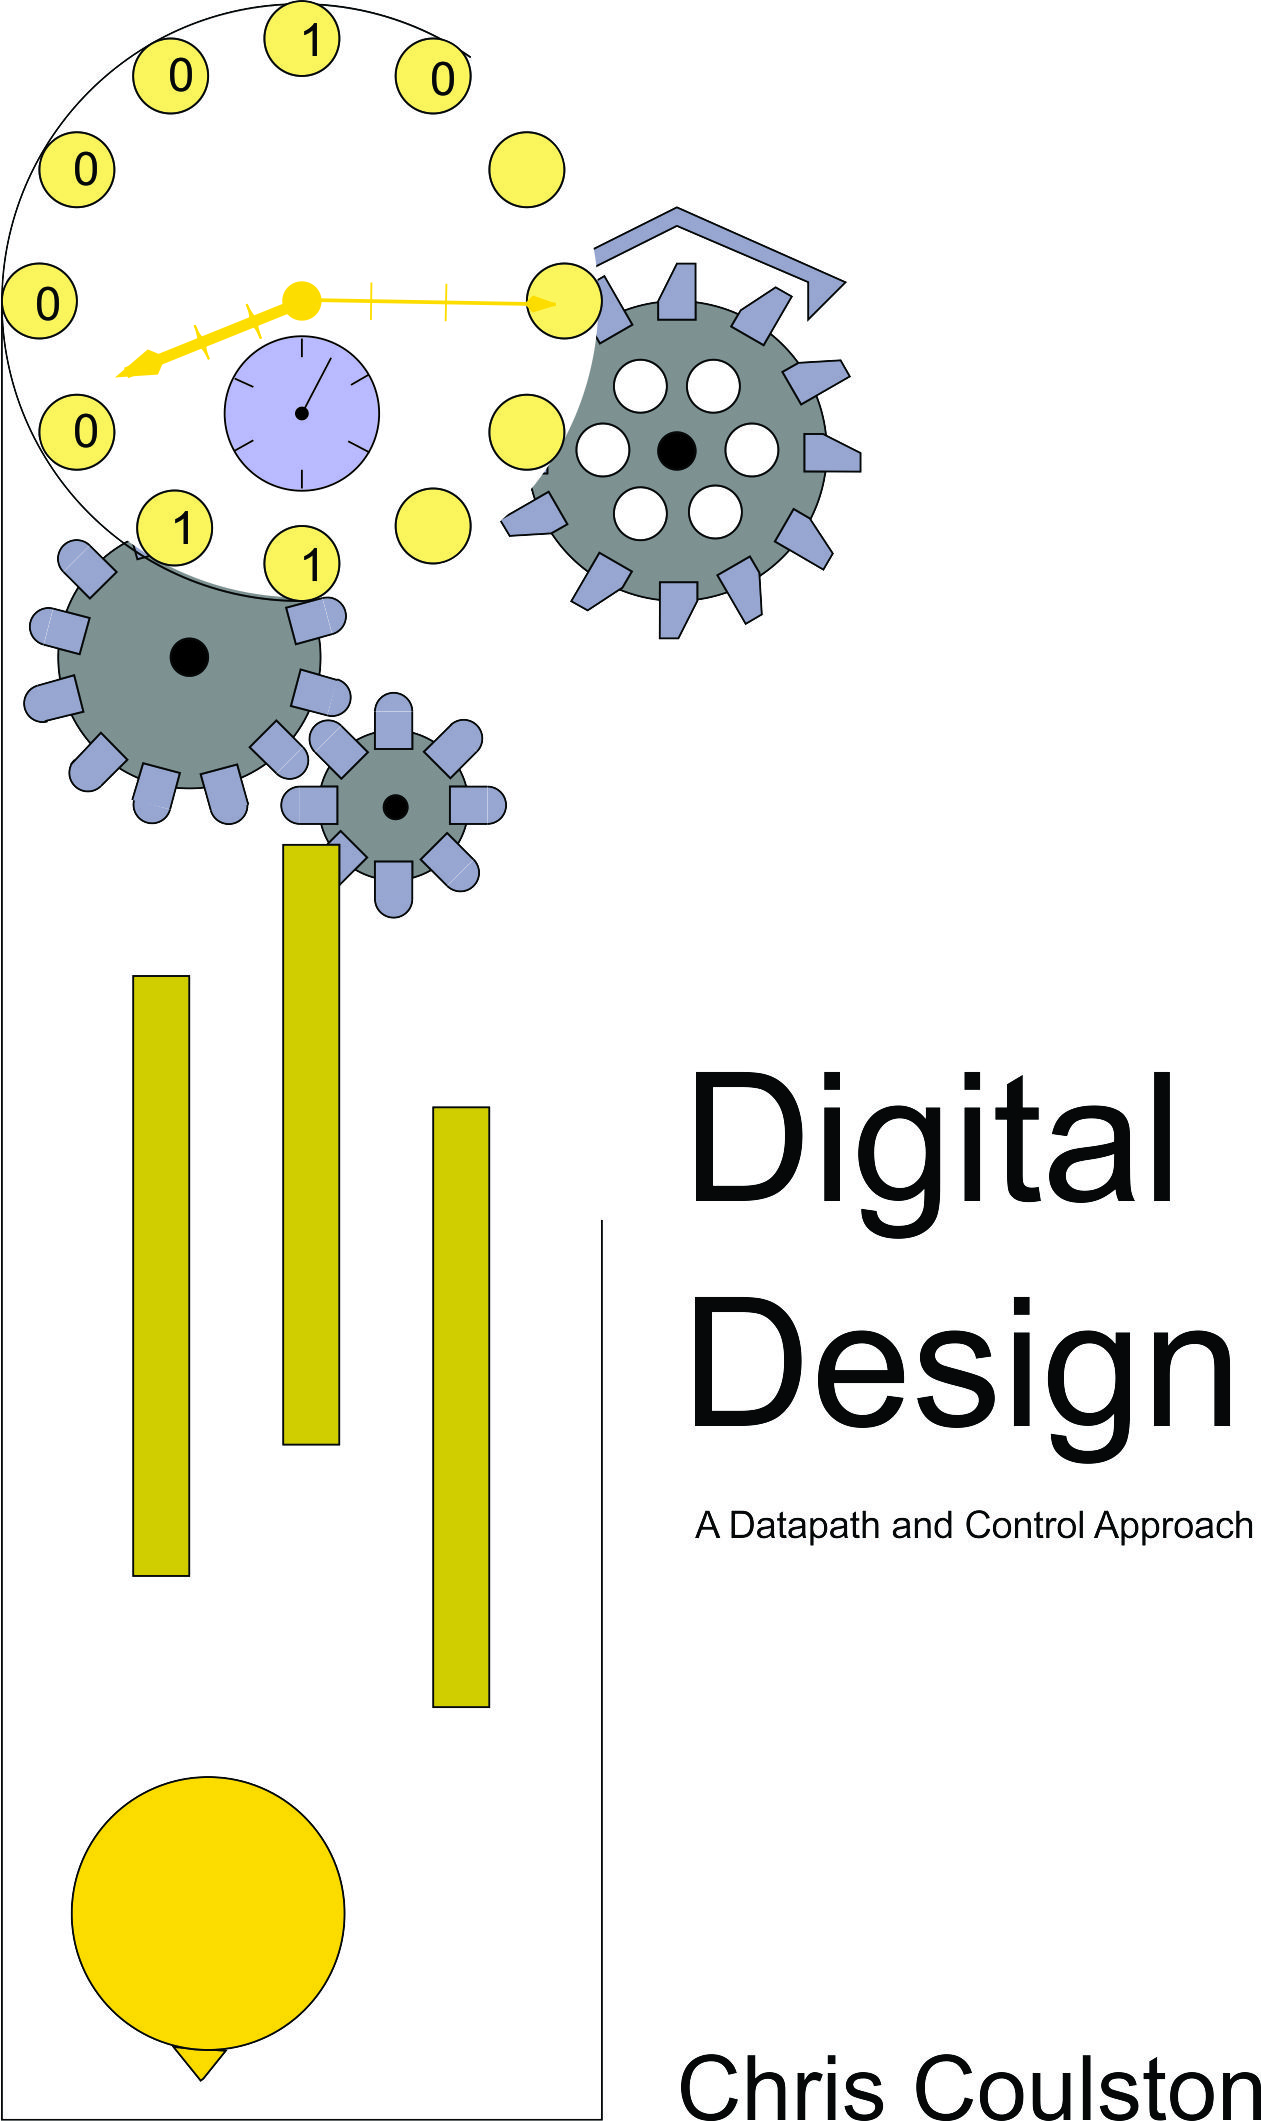
\includegraphics{./Fig/colorCover}
\maketitle

This document was prepared with \LaTeX.
\vspace{2cm}

Digital Design - A Datapath and Control Approach © 2024 by Christopher Coulston is licensed under CC BY-NC-SA 4.0
For more infomation about the Create Commons license see: https://creativecommons.org/licenses/by-nc-sa/4.0/

\begin{figure}[h]
    
\includegraphics[width=1cm]{./Fig/cc-logo.pdf}
    
\includegraphics[width=1cm]{./Fig/cc-by.pdf}
    
\includegraphics[width=1cm]{./Fig/cc-nc.pdf}
    
\includegraphics[width=1cm]{./Fig/cc-sa.pdf}
\end{figure}

\tableofcontents
\showanswers

\mainmatter
\chapter*{Homework Solutions}

%\setcounter{chapter}{0}
%\setcounter{section}{-1}
\chapter{Numbering Systems}
\section{Exercises}
\label{section:chap01Exercises}

\begin{enumerate}
\item \textbf{ (1 pt. each)} Syllabus:
	\begin{enumerate}
	\item What is the late penalty for homework?
	
	\begin{onlysolution}
	\itshape
	There is a 33\% deduction per day.
	\end{onlysolution}

	\item True or False: Calculators can be used during exams.
	
	\begin{onlysolution}
	\itshape
	You cannot use calculators at my exams.
	\end{onlysolution}
	
	
	\item True of False: University ID is required during exams.
	
		
	\begin{onlysolution}
	\itshape
	I check ID at the exams.  After I learn 
		your names its not such a big
		deal, but bring it to be safe.
	\end{onlysolution}
	
	\item What is my thesis regarding grades?
	\item Bob L. Student has the following grades.  Determine his final
	overall course percentage and grade.

		\begin{tabular}{l|l}
		Component & Percentage \\ \hline \hline
		Homework & $60\%$ \\ \hline
		Exam 1	 & $90\%$ \\ \hline
		Exam 2	 & $80\%$ \\ \hline
		Final	 & $70\%$ \\ 
		\end{tabular}


	\begin{onlysolution}
	\itshape
                \begin{tabular}{l|l|l}
                Component & Percentage & Weight \\ \hline \hline
                Homework & $60\%$    & 60*0.35 = 21\\ \hline
                Exam 1   & $90\%$    & 90*0.20 = 18\\ \hline
                Exam 2   & $80\%$    & 80*0.20 = 16\\ \hline
                Final    & $70\%$    & 70*0.25 = 17.5 \\ \hline
                Total    & $72.5\%$ & C \\
                \end{tabular}
	\end{onlysolution}

	\item How should you prepare for the 43$^{rd}$ lecture?

	\begin{onlysolution}
	\itshape
	 Look over homework problem 8.10, page 165
	 \end{onlysolution}
	 
	\end{enumerate}

\item \textbf{ (1 pt. each)} Convert the following numbers to decimal. 
Show work, or receive 1/2 credit.
	\begin{enumerate}
	\item $100_2$
	\begin{onlysolution}	\itshape $100_2 = 2^2 = 4_{10}$\end{onlysolution}
	
	\item $1000_2$
	\begin{onlysolution}	\itshape $1000_2 = 2^3 = 8_{10}$\end{onlysolution}
	
	\item $10000_2$
	\begin{onlysolution}	\itshape $10000_2 = 2^4 = 16_{10}$\end{onlysolution}
	
	\item $100000_2$
	\begin{onlysolution}	\itshape $100000_2 = 2^5 = 32_{10}$\end{onlysolution}
	
	\item $111111_2$
	\begin{onlysolution}	\itshape $111111_2 = 2^5+2^4+2^3+2^2+2^1+2^0=63_{10}$\end{onlysolution}
	
	\item $1000100101000101_2$
	\begin{onlysolution}	\itshape $1000100101000101_2=2^{15}+2^{11}+2^8+2^6+2^5+2^0=35141_{10}$\end{onlysolution}
	
	\item $3EA_{16}$
	\begin{onlysolution}	\itshape$3EA_{16}=0011 1110 1010 = 2^9+2^8+2^7+2^6+2^5+2^3+2^1=1002_{10}$\end{onlysolution}
	
     \end{enumerate}


\item \textbf{ (1 pt. each)} Convert the following number to binary. Show 
work, or receive 1/2 credit.
	\begin{enumerate}
	\item $44_{16}$
	\begin{onlysolution}	\itshape $44_{16} =0100 0100_2$\end{onlysolution}
	
	\item $44_{10}$
	\begin{onlysolution}	\itshape $44_{10} = 32+8 = 2^5+2^3=101100_2$\end{onlysolution}
	
	\item $1023_{10}$
	\begin{onlysolution}	\itshape$1023_{10} = 512+256+128+64+32+16+8+4+2+1=
        2^9+2^8+2^7+2^6+2^5+2^4+2^3+2^2+2^1+2^0=1111111111_2$\end{onlysolution}
        
	\end{enumerate}


\item \textbf{ (1 pt. each)} Convert the following number to hex. Show work, or receive 1/2 credit.
	\begin{enumerate}
	
	\item $101011101_2$
	\begin{onlysolution}	\itshape$1 0101 1101_2 = 15D_{16}$ \end{onlysolution}
	
	\item $77_{10}$
	\begin{onlysolution}	\itshape $77_{10} = 64+8+4+1=2^6+2^3+2^2+2^0=100 1101_2=4D_{16}$ \end{onlysolution}
	
	\end{enumerate}


\item \textbf{ (2 pts. each)} Toughies:
	\begin{enumerate}
	\item Convert $123_5$ to base-12
	\begin{onlysolution} 	\itshape
		$123_5 = 1*5^2 + 2*5^1 + 3*5^0 = 25+10+3=38_{10}=
        3*12^1 + 2*12^0 = 32_{12}$ \end{onlysolution}
        
	\item Convert $789_{12}$ to base-5
	\begin{onlysolution}
	\itshape	$789_{12} = 7*12^2+8*12^1+9*12^0=1008+96+9=1113_{10}= \\
        1*5^4+3*5^3 + 4*5^2 + 2*5^1 + 3*5^0 = 13423_5$ \end{onlysolution}
        
	\item What is the largest base-10 quantity that can be represented
	using 5 digits in base 12?

	\begin{onlysolution}
	\itshape $BBBBB_{12} = 11*12^4+11*12^3+11*12^2+11*12^1+11*12^0=248831_{10}$ \end{onlysolution}
	
	\end{enumerate}


\item \textbf{ (1 pt. each)} Perform the following additions, assume a word 
size of four bits. Determine if overflow occurs.
	\begin{enumerate}
	
	\item $0110_2 + 0101_2$
	\begin{onlysolution}	\itshape0110 + 0101 = 1011\end{onlysolution}
	
	\item $0010_2 + 0110_2$
	\begin{onlysolution}	\itshape0010 + 0110 = 1000\end{onlysolution}
	
	\item $0111_2 + 0011_2$
	\begin{onlysolution}	\itshape0111 + 0011 = 1010\end{onlysolution}
	
	\item $0010_2 + 0101_2$
	\begin{onlysolution}	\itshape0010 + 0101 = 0111\end{onlysolution}
	
	\item $0010_2 + 1010_2$
	\begin{onlysolution}	\itshape0010 + 1010 = 1100\end{onlysolution}
	
	\item $0101_2 + 1011_2$
	\begin{onlysolution}	\itshape0101 + 1011 = 10000 overflow\end{onlysolution}
	
	\item $0011_2 + 1001_2$
	\begin{onlysolution}	\itshape0011 + 1001 = 1100\end{onlysolution}
	
	\end{enumerate}
\end{enumerate}


%\setcounter{chapter}{1}
%\setcounter{section}{01}
\chapter{Representations of Logical Functions}
\begin{enumerate}
\item {\bf(2 pts. each)} Given: $F(A,B,C,D) = (AB' + (C+(AD)')(BD))'$
\begin{enumerate}
	\item Determine the truth table for $F(A,B,C,D)$

\begin{solution}{ 
Let T3 = C+(AD)'\\
T4 = BD\\
T1 = AB'
T5 = T3 * T4\\

\begin{tabular}{l|l|l|l|l|l|l|l|l|l|l} 
 A &  B &  C &  D & AB' & (AD)' & C+(AD)' & BD & T3*T4 & T1+T5  &  F \\ \hline
 0 &  0 &  0 &  0 &  0  &  1    &  1      &  0 & 0     &  0     &  1  \\ \hline
 0 &  0 &  0 &  1 &  0 &  1 &  1 &  0 & 0 &  0 &  1  \\ \hline
 0 &  0 &  1 &  0 &  0 &  1 &  1 &  0 & 0 &  0 &  1  \\ \hline
 0 &  0 &  1 &  1 &  0 &  1 &  1 &  0 & 0 &  0 &  1  \\ \hline
 0 &  1 &  0 &  0 &  0 &  1 &  1 &  0 & 0 &  0 &  1  \\ \hline
 0 &  1 &  0 &  1 &  0 &  1 &  1 &  1 & 1 &  1 &  0  \\ \hline
 0 &  1 &  1 &  0 &  0 &  1 &  1 &  0 & 0 &  0 &  1  \\ \hline
 0 &  1 &  1 &  1 &  0 &  1 &  1 &  1 & 1 &  1 &  0  \\ \hline
 1 &  0 &  0 &  0 &  1 &  1 &  1 &  0 & 0 &  1 &  0  \\ \hline
 1 &  0 &  0 &  1 &  1 &  0 &  0 &  0 & 0 &  1 &  0  \\ \hline
 1 &  0 &  1 &  0 &  1 &  1 &  1 &  0 & 0 &  1 &  0  \\ \hline
 1 &  0 &  1 &  1 &  1 &  0 &  1 &  0 & 0 &  1 &  0  \\ \hline
 1 &  1 &  0 &  0 &  0 &  1 &  1 &  0 & 0 &  0 &  1  \\ \hline
 1 &  1 &  0 &  1 &  0 &  0 &  0 &  1 & 0 &  0 &  1  \\ \hline
 1 &  1 &  1 &  0 &  0 &  1 &  1 &  0 & 0 &  0 &  1  \\ \hline
 1 &  1 &  1 &  1 &  0 &  0 &  1 &  1 & 1 &  1 &  0  \\  
\end{tabular} 
} \end{solution}

	\item Draw a schematic of the logic circuit which realizes $F$ as
	shown, i.e. do not use Boolean Algebra on $F$.

\begin{solution}{
	\begin{figure}[ht]
	\center{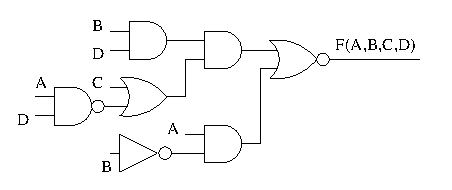
\includegraphics{./FigHw2/Sol2-1}}
	\end{figure}
}\end{solution}
\end{enumerate}


\item {\bf(2 pts. each)} For the circuit in Figure~\ref{fig:hw2}: 
\begin{enumerate}
	\item Write a Boolean expression for the function.

	\begin{solution}{ F(A,B,C,D) = (AB+C)D'+ABD'}\end{solution}
\item Draw the truth table for the function.


	\begin{solution}{
	\begin{tabular}{l|l|l|l|l|l|l|l}
	 A &  B &  C &  D & AB+C  & (AB+C)D' & ABD'  &  F  \\ \hline
	 0 &  0 &  0 &  0 &  0 &  0 &  0 &  0  \\ \hline
	 0 &  0 &  0 &  1 &  0 &  0 &  0 &  0  \\ \hline
	 0 &  0 &  1 &  0 &  1 &  0 &  0 &  1  \\ \hline
	 0 &  0 &  1 &  1 &  1 &  1 &  0 &  0  \\ \hline
	 0 &  1 &  0 &  0 &  0 &  0 &  0 &  0  \\ \hline
	 0 &  1 &  0 &  1 &  0 &  0 &  0 &  0  \\ \hline
	 0 &  1 &  1 &  0 &  1 &  0 &  0 &  1  \\ \hline
	 0 &  1 &  1 &  1 &  1 &  1 &  0 &  0  \\ \hline
	 1 &  0 &  0 &  0 &  0 &  0 &  0 &  0  \\ \hline
	 1 &  0 &  0 &  1 &  0 &  0 &  0 &  0  \\ \hline
	 1 &  0 &  1 &  0 &  1 &  0 &  0 &  1  \\ \hline
	 1 &  0 &  1 &  1 &  1 &  1 &  0 &  0  \\ \hline
	 1 &  1 &  0 &  0 &  1 &  0 &  1 &  1  \\ \hline
	 1 &  1 &  0 &  1 &  1 &  1 &  0 &  0  \\ \hline
	 1 &  1 &  1 &  0 &  1 &  0 &  1 &  1  \\ \hline
	 1 &  1 &  1 &  1 &  1 &  0 &  0 &  0  \\ 
	\end{tabular}
}\end{solution}
\end{enumerate}
\begin{figure}[ht]
\center{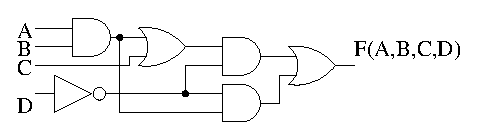
\includegraphics{./FigHw2/Prob2-3}}
\caption{The circuit for Problems 2 and 3.}
\label{fig:hw2}
\end{figure}

\item {\bf(2 pts.)} For the circuit in Figure~\ref{fig:hw2}, show what 
happens when the input (A,B,C,D)=0010 is switched to (A,B,C,D)=1101.
Assume the first input (0010) has been held steady
for a long time.  Use a timing diagram and assume that 
the propagation delay of each gate is 2nS.

	\begin{solution}{ Skipped, a glitch is created for sure.}\end{solution}

\item {\bf (2 pts. each)} For the functions F,G,H,I defined by the 
truth table shown below:
\begin{enumerate}
	\item Determine the canonical SOP and POS realization for $F,G,H,I$.

	\begin{solution}{
F(A,B,C) = (A+B+C)(A+B'+C')(A'+B+C')(A'+B'+C)  =
A'B'C + A'BC' + AB'C' + ABC \\

G(A,B,C) = (A'+B+C)(A'+B'+C') = \\
A'B'C' + A'B'C + A'BC' + A'BC + AB'C + ABC'  \\

H(A,B,C) = (A+B'+C)(A+B'+C')(A'+B+C)(A'+B+C')(A'+B'+C') =\\
A'B'C' + A'B'C + ABC' \\

I(A,B,C) = (A+B+C)(A+B'+C)(A'+B+C)(A'+B'+C) =\\
A'B'C + A'BC + AB'C + ABC \\
}\end{solution}

	\item Draw the circuit diagram for the canonical SOP and POS 
		realization.

	\begin{solution}{
	\begin{figure}[ht]
	\center{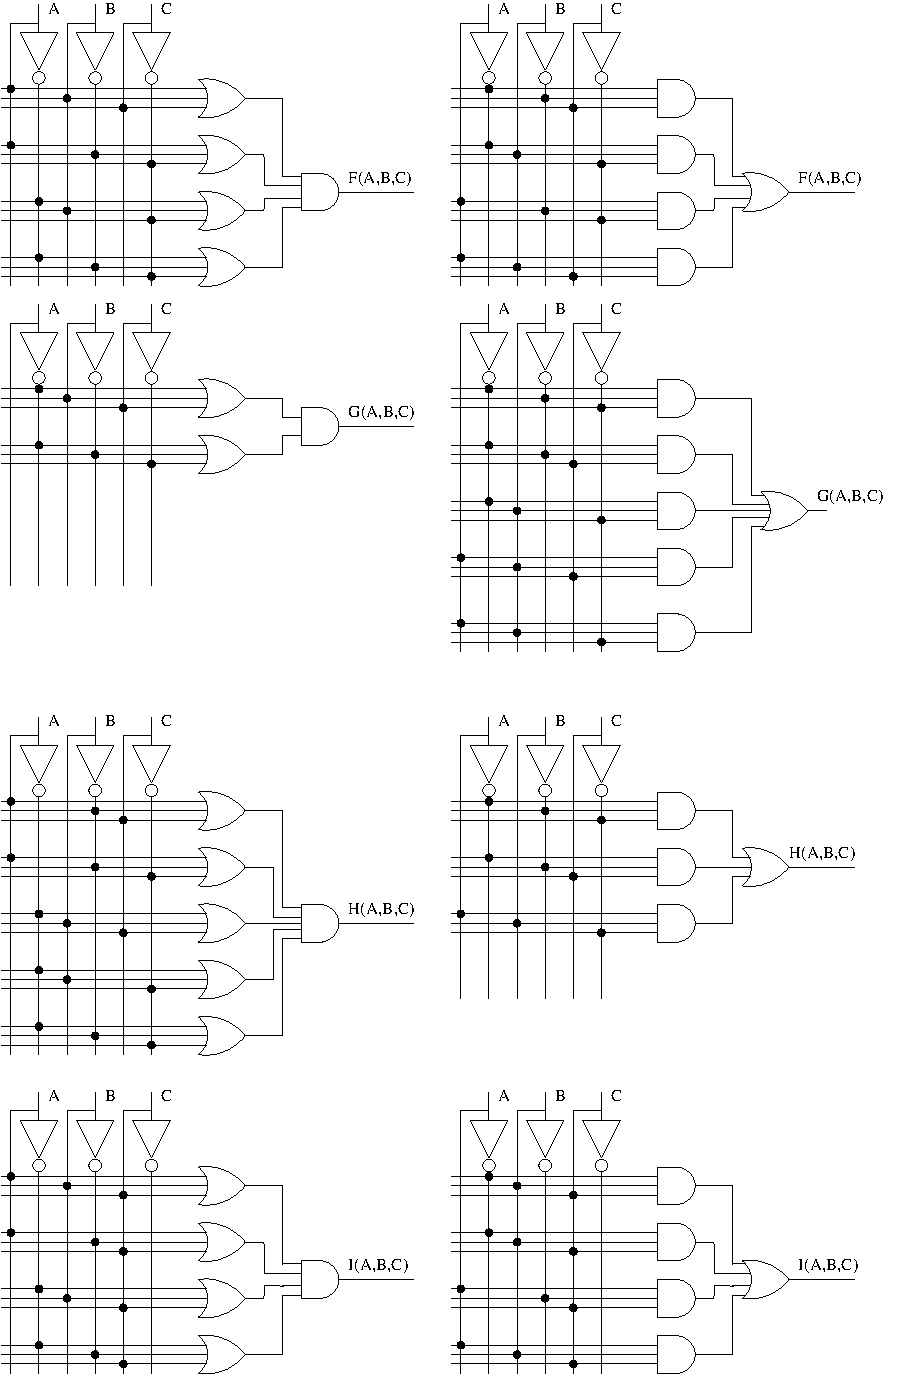
\includegraphics{./FigHw2/Sol2-4}}
	\end{figure}
}\end{solution}
\end{enumerate}
Treat each output independently of the other.  For example when
working with function $I$, cover up the columns $F,G$ and $H$.

$$\begin{array}{c|c|c||c|c|c|c}
 	A & B & C & F & G & H & I \\ \hline
 	0 & 0 & 0 & 0 & 1 & 1 & 0 \\ \hline
 	0 & 0 & 1 & 1 & 1 & 1 & 1 \\ \hline
 	0 & 1 & 0 & 1 & 1 & 0 & 0 \\ \hline
 	0 & 1 & 1 & 0 & 1 & 0 & 1 \\ \hline
 	1 & 0 & 0 & 1 & 0 & 0 & 0 \\ \hline
 	1 & 0 & 1 & 0 & 1 & 0 & 1 \\ \hline
 	1 & 1 & 0 & 0 & 1 & 1 & 0 \\ \hline
 	1 & 1 & 1 & 1 & 0 & 0 & 1 \\
\end{array}$$

\item  {\bf (2 pts. each)} Prove the validity of the following 
statements using the laws of Boolean Algebra. For each step of 
the proof, identify which law was used.
\begin{enumerate}
	\item $X'Y' + XY + X'Y = X' + Y$

\begin{solution}{
\begin{tabular}{lr}
X'Y' + XY + X'Y = 	& 3D\\
X'Y' + X'Y + XY+ X'Y =	& 8 \\
X'(Y' + Y )+ Y(X+ X')Y=	& 5 \\
X' + Y 			& QED \\
\end{tabular} }\end{solution}

	\item $(X+Y')X'Y' = X'Y'$

\begin{solution}{
\begin{tabular}{lr}
(X+Y')X'Y' = 	& 8 \\
XX'Y + X'Y'Y' = & 5D \\
0+X'Y'= 	& 1 \\
X'Y' 		& QED \\
\end{tabular}}\end{solution}

	\item $(X+Y)(X'+Z) = XZ + X'Y$

\begin{solution}{
\begin{tabular}{lr}
(X+Y)(X'+Z) = 		& 8 \\
(X+Y)X' + (X+Y)Z = 	& 8 \\
XX' + YX' + XZ + YZ =	& 1D,5 \\
YX' + XZ + YZ(X+X') =  	& 8 \\
YX' + XZ + XYZ + X'YZ =	& 6  \\
X'Y + X'YZ + XZ + XYZ =	& 1D, 8 \\
X'Y(1+Z) + XZ(1+Y) =  	& 2, 1D \\
X'Y + XZ 		& QED \\
\end{tabular} }\end{solution}

	\item $X'Y' + (X+Y)Z = X'Y' + Z$

\begin{solution}{
\begin{tabular}{lr}
X'Y' + (X+Y)Z = 				& 8\\
X'Y' + XZ + YZ = 				& 1D,5 \\
X'Y'*(Z+Z') + XZ + YZ(X+X') =  			& 8 \\
X'Y'Z' + X'Y'Z + XZ + XYZ + X'YZ =  		& 3 \\
X'Y'Z' + X'Y'Z + X'Y'Z + XZ + XYZ + X'YZ =  	& 8 \\
X'Y'(Z+Z') + XZ(1+Y) + X'Z(Y'+Y) =  		& 5,1D \\
X'Y' + XZ + X'Z  =  				& 8 \\
X'Y' + Z(X+X') =  				& 5, 1D\\
X'Y' + Z 					& QED \\
\end{tabular} }\end{solution}

	\item $A'C+BC+AB = A'C+AB$

\begin{solution}{
\begin{tabular}{lr}
A'C + BC+AB =  					& 1D, 5 \\
A'C + (A+A')BC + AB(C+C') 			& 8  \\
A'C + ABC + A'BC + ABC + ABC'= 			& 3\\
A'C + A'BC + ABC + ABC'= 			& 8\\
A'C(1+B) + AB(C+C')= 				& 5, 1D\\
A'C + AB 					& QED \\
\end{tabular} }\end{solution}
	\item $A(B+C)=AB+AB'C$

\begin{solution}{
\begin{tabular}{lr}
AB+AB'C= 					& 1D,5\\
AB(C+C') + AB'C= 				& 8 \\
ABC+ABC'+AB'C= 					& 3 \\
ABC + ABC + ABC' + AB'C= 			& 6\\
ABC + ABC' + ABC + AB'C= 			& 8\\
AB(C+C'+C) + AB'C = 				& 8\\	
AB + AB'C= 					& QED\\
\end{tabular}	}\end{solution}
	\item $(A+B+C)(A+B+C')(A'+B+C')(A'+B'+C') = (A+B)(A'+C')$

\begin{solution}{
\begin{tabular}{lr}
(A+B+C)(A+B+C')(A'B+C')(A'+B'+C')= 		& 4\\
((A+B+C)(A+B+C')(A'B+C')(A'+B'+C'))''= 		& 9D\\
(A'B'C + A'B'C' + AB'C + ABC)'= 		& 8\\
(A'B'(C+C') + AC(B'+B))'= 			& 5, 1D\\
(A'B' + AC)'= 					& 9 \\
(A+B)(A'+C')= 					& QED \\
\end{tabular}	}\end{solution}
\end{enumerate}

\item {\bf (4 pts.)} Design a circuit called MUX2.  MUX2 has three bits 
of input $S, y_0, y_1$ and one bit of output $F$.  If $S=0$, then 
$F=y_0$; else if $S=1$, then $F=y_1$.
\begin{enumerate}
	\item Write down the truth table for the MUX2 function.

\begin{solution}{
	\begin{tabular}{l|l|l|l}
	S & y0 &  y1 & F \\ \hline
	0 & 0  &  0  & 0 \\ \hline
	0 & 0  &  1  & 0 \\ \hline
	0 & 1  &  0  & 1 \\ \hline
	0 & 1  &  1  & 1 \\ \hline
	1 & 0  &  0  & 0 \\ \hline
	1 & 0  &  1  & 1 \\ \hline
	1 & 1  &  0  & 0 \\ \hline
	1 & 1  &  1  & 1 \\ 
	\end{tabular}
}\end{solution}

	\item Determine the canonical SOP realization for MUX2; 
		do not simplify.

\begin{solution}{F = S'y0y1' + S'y0y1 + Sy0'y1 + Sy0y1}\end{solution}
\end{enumerate}

\item {\bf (6 pts.)} Design a circuit called MUX4.  MUX4 has six bits of input 
$S_1 S_0, y_0, y_1, y_2, y_3$ and one bit of output $F$.  \\
If      $S_1 S_0 = 00$ then $F=y_0$  \\
else if $S_1 S_0 = 01$ then $F=y_1$ \\
else if $S_1 S_0 = 10$ then $F=y_2$ \\
else if $S_1 S_0 = 11$ then $F=y_3$ \\
Without writing down the truth table determine a SOP expression
to realize F by listing all possible inputs which will cause F to equal 1.
Then try to simplify your expression using Boolean Algebra.

\begin{solution}{
The output F only equals one in the following cases.
\begin{description}
\item S1=0 S0=0 and y0=1
\item S1=0 S0=1 and y1=1
\item S1=1 S0=0 and y2=1
\item S1=1 S0=1 and y3=1
\end{description}

With this information we can form four product terms, one for each input, 
that equal 1 only for that input.  ORing together these product terms 
will give us the solution to the problem.

$F = S_1'S_0'y_0 + S_1'S_0 y_1 + S_1 S_0'y_2 + S_1 S_0 y_3$
} \end{solution}

\item  {\bf (4 pts.)} Design a logic circuit called {\it MAJ} which 
has three inputs $A,B,C$ and one output $Z$. The output equals 1 
when a majority of the inputs are equal to 1, otherwise the output is 0.
\begin{enumerate}
	\item Write the truth table for the MAJ function.

\begin{solution}{
	\begin{tabular}{l|l|l||l} \\ 
	A & B & C &  F \\ \hline
	0 & 0 & 0 &  0 \\ \hline
	0 & 0 & 1 &  0 \\ \hline
	0 & 1 & 0 &  0 \\ \hline
	0 & 1 & 1 &  1 \\ \hline
	1 & 0 & 0 &  0 \\ \hline
	1 & 0 & 1 &  1 \\ \hline
	1 & 1 & 0 &  1 \\ \hline
	1 & 1 & 1 &  1 \\ 
	\end{tabular}
}\end{solution}
	\item Determine the canonical SOP realization for the MAJ
	function, do not simplify.

\begin{solution}{ F = A'BC + AB'C+ABC'+ABC} \end{solution}
\end{enumerate}

\item {\bf (4 pts.)} Let $X$ and $Y$ each be 2-bit signals whose 
elements are $x_1 x_0$ and $y_1 y_0$ respectively.  Determine the 
$\sum m$ and $\prod M$ expression for a circuit whose 1-bit 
output $z$ is defined by the following statement.
\begin{verbatim}
	if (X == Y) then z = 1 else z =0
\end{verbatim}

\begin{solution}{
The truth table for the solution is shown below.
$$\begin{array}{c|c|c|c||c|c||c}
a_1 & a_0 & b_1 & b_0 & A  & B & z  \\ \hline
0 & 0 & 0 & 0 & 0 & 0 & 1  \\ \hline
0 & 0 & 0 & 1 & 0 & 1 & 0  \\ \hline
0 & 0 & 1 & 0 & 0 & 2 & 0  \\ \hline
0 & 0 & 1 & 1 & 0 & 3 & 0  \\ \hline
0 & 1 & 0 & 0 & 1 & 0 & 0  \\ \hline
0 & 1 & 0 & 1 & 1 & 1 & 1  \\ \hline
0 & 1 & 1 & 0 & 1 & 2 & 0  \\ \hline
0 & 1 & 1 & 1 & 1 & 3 & 0  \\ \hline
1 & 0 & 0 & 0 & 2 & 0 & 0  \\ \hline
1 & 0 & 0 & 1 & 2 & 1 & 0  \\ \hline
1 & 0 & 1 & 0 & 2 & 2 & 1  \\ \hline
1 & 0 & 1 & 1 & 2 & 3 & 0  \\ \hline
1 & 1 & 0 & 0 & 3 & 0 & 1  \\ \hline
1 & 1 & 0 & 1 & 3 & 1 & 0  \\ \hline
1 & 1 & 1 & 0 & 3 & 2 & 0  \\ \hline
1 & 1 & 1 & 1 & 3 & 3 & 1  \\
\end{array}$$

The solution is shown below.

$z = \sum m(0,5,10,15) = \prod M(1,2,3,4,6,7,8,9,11,12,13,14)$
} \end{solution}


\item {\bf (4 pts.)} Let $X$ and $Y$ each be 2-bit signals whose 
elements are $x_1 x_0$ and $y_1 y_0$, respectively.  Determine the 
$\sum m$ and $\prod M$ expressions for a circuit whose 1-bit
output $z$ is defined by the following statement.
\begin{verbatim}
        if (X + Y > 3) then z = 0 else z =1
\end{verbatim}

\begin{solution}{
The truth table for the problem is shown below
$$\begin{array}{c|c|c|c||c|c||c}
a_1 & a_0 & b_1 & b_0 & A  & B & z  \\ \hline
0 & 0 & 0 & 0 & 0 & 0 & 1  \\ \hline
0 & 0 & 0 & 1 & 0 & 1 & 1  \\ \hline
0 & 0 & 1 & 0 & 0 & 2 & 1  \\ \hline
0 & 0 & 1 & 1 & 0 & 3 & 1  \\ \hline
0 & 1 & 0 & 0 & 1 & 0 & 1  \\ \hline
0 & 1 & 0 & 1 & 1 & 1 & 1  \\ \hline
0 & 1 & 1 & 0 & 1 & 2 & 1  \\ \hline
0 & 1 & 1 & 1 & 1 & 3 & 0  \\ \hline
1 & 0 & 0 & 0 & 2 & 0 & 1  \\ \hline
1 & 0 & 0 & 1 & 2 & 1 & 1  \\ \hline
1 & 0 & 1 & 0 & 2 & 2 & 0  \\ \hline
1 & 0 & 1 & 1 & 2 & 3 & 0  \\ \hline
1 & 1 & 0 & 0 & 3 & 0 & 1  \\ \hline
1 & 1 & 0 & 1 & 3 & 1 & 0  \\ \hline
1 & 1 & 1 & 0 & 3 & 2 & 0  \\ \hline
1 & 1 & 1 & 1 & 3 & 3 & 0  \\
\end{array}$$
Leading to this answer
$ z = \sum m(0,1,2,3.4,5,6,8,12) = \prod M(7,9,10,11,13,14,15)$
}\end{solution}

	

\item {\bf (3 pts.)} Determine the canonical SOP and POS expression for 
$F(A,B,C) = \prod M (0,1,4,5)$  Hint, compose the truth table for $F$.

\begin{solution}{
F(A,B,C)=A'BC' + A'BC +ABC' +ABC  \\
F(A,B,C)=(A+B+C)(A+B+C')(A'+B+C)(A'+B+C')
}\end{solution}

\item {\bf (3 pts.)} Determine the canonical SOP and POS expression for 
$F(A,B,C,D) = \sum m(0,4,12,15)$ Hint, write out the truth table for $F$.

\begin{solution}{
F(A,B,C)=A'B'C'D' + A'BC'D' + ABC'D' + ABCD  \\
F(A,B,C)=(A+B+C+D')(A+B+C'+D)(A+B+C'+D') (A+B'+C+D')(A+B'+C'+D) \\
(A+B'+C'+D')(A'+B+C+D)(A'+B+C+D') (A'+B+C'+D)(A'+B+C'+D')(A'+B'+C+D')\\
(A'+B'+C'+D)
}\end{solution}

\item {\bf (4 pts.)} For the function $F(A,B,C)= BC+AB'C'$,  draw
a timing diagram for an input sequence that follows the same order 
as the rows of the truth table.  Assume a propagation delay for NOT, 
AND and OR gate are all 10nS.

	\begin{solution}{skipped for now}\end{solution}

\item {\bf (4 pts.)} Complete the timing diagram in Figure~\ref{fig:HWtime}
for the functions
$F(A,B,C) = AB' + BC + ABC'$ and $G(A,B,C) = (A+B')C + (BC')'$
\begin{figure}[ht]
\center{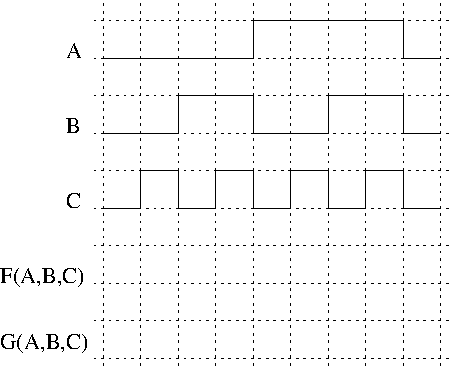
\includegraphics{./FigHw2/Prob2-14}}
\caption{The timing diagram for two functions, $F$ and $G$.}
\label{fig:HWtime}
\end{figure}

\begin{solution}{

\begin{figure}[ht]
\center{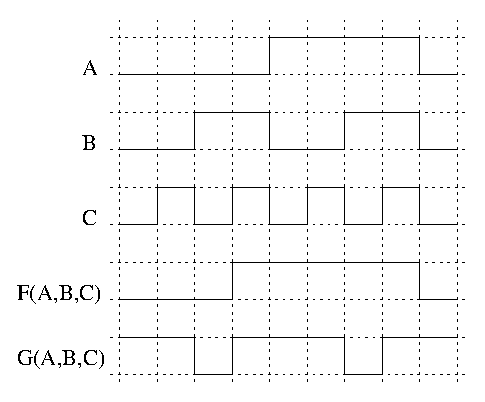
\includegraphics{./FigHw2/Sol2-14}}
\end{figure}
}\end{solution}

\item{\bf (16 pts.)} Design a circuit to control
the water pump of a washing machine.  The pump will not pump 
water if
\begin{description}
\item The lid is closed and the cycle is not fill
\item The cycle is fill and the detergent level is empty
\item The detergent is not empty and the lid is open
\end{description}
                                                                                
The variables for this problem are:
\begin{description}
\item L = lid is closed
\item C = cycle is fill
\item D = detergent is empty
\item P = pump will pump water
\end{description}
                                                                                
                                                                                
Create a truth table which describes when the pump will not
pump water.  Call this output P'.  Determine the canonical SOP
expression for P'.  Use this canonical SOP expression to generate
a circuit diagram for P.  This can be done by inserting an
inverter onto the output of the circuit.
                                                                                
Take the P' column from truth table and invert all the entries
to generate a new output column called P (because
the negation of P' is P).  Determine the canonical SOP
realization for P using this new column.
\end{enumerate}


%\setcounter{chapter}{3}
%\setcounter{section}{-1}
\chapter{Minimization of Logical Functions}
\begin{enumerate}
\item {\bf (6 pts.)} Design a circuit called DECODE.  DECODE has two bits of 
input $S, D$ and two bit of output $y_1 y_0$.  If $S=0$ then $y_0=D$ and 
$y_1=0$ else if $S=1$ then $y_0=0$ and $y_1 = D$.
\begin{enumerate}
        \item Write down the truth table for the DECODE function.


\begin{solution}{
	\begin{tabular}{l|l||l|l}
	S & D & $y_1$ & $y_0$ \\ \hline
	0 & 0 & 0   & 0   \\ \hline
	0 & 1 & 0   & 1   \\ \hline
	0 & 0 & 0   & 0   \\ \hline
	1 & 1 & 1   & 0   \\ 
	\end{tabular}
} \end{solution}
        \item Determine the \SOPmin realization for DECODE.


\begin{solution}{
$y_0 = S'D$\\
$y_1 = S D$
} \end{solution}
\end{enumerate}

\item {\bf (6 pts.)} Design a circuit called FULLADD.  FULLADD has 
three bits of input $a,b,c$ and two bits of output $s_1 s_0$.  The output 
represents the sum of the three bits.
\begin{enumerate}
        \item Write down the truth table for the FULLADD function.


\begin{solution}{
	\begin{tabular}{l|l|l|l|l}
	a & b & c & $s_1$ & $s_0$ \\ \hline
	0 & 0 & 0 & 0   & 0   \\ \hline
	0 & 0 & 1 & 0   & 1   \\ \hline
	0 & 1 & 0 & 0   & 0   \\ \hline
	0 & 1 & 1 & 1   & 1   \\ \hline
	1 & 0 & 0 & 0   & 0   \\ \hline
	1 & 0 & 1 & 1   & 1   \\ \hline
	1 & 1 & 0 & 1   & 0   \\ \hline
	1 & 1 & 1 & 1   & 1   \\ 
\end{tabular}
} \end{solution}
        \item Determine the \SOPmin realization for FULLADD.

\begin{solution}{
$s_1 = ab + ac + bc $ \\
$s_0 = a'b'c + a'bc' + ab'c' + abc $
} \end{solution}
\end{enumerate}

\item  {\bf (4 pts.)} Determine \SOPmin expression for the following circuit
and draw the circuit using the fewest number of gates possible.
\begin{figure}[ht]
%% scalebox
\center{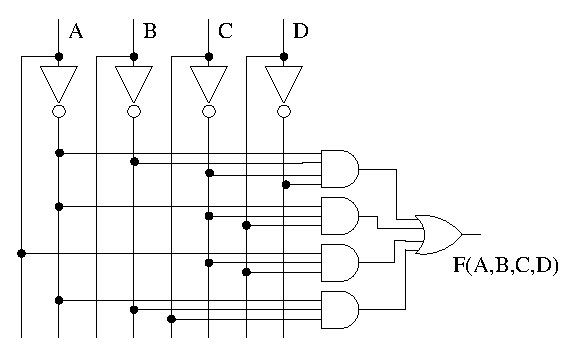
\includegraphics{./FigHw3/Prob3-3}}
\label{fig:Hw3}
\end{figure}

\begin{solution}{
From the circuit we have:
F(A,B,C,D) = A'B'C'D' + A'C'D + AC'D + A'B'C
$$ \begin{array} {c||c|c|c|c}
       AB \bs CD & 00 & 01 & 11 & 10 \\ \hline \hline
       00        & 1  & 1  & 1  & 1  \\ \hline
       01        &    & 1  &    &    \\ \hline
       11        &    & 1  &    &    \\ \hline
       10        &    & 1  &    &    \\
\end{array} $$ 
From this it follows that 
F(A,B,C,D) =  A'B' + C'D
} \end{solution}

\item  {\bf (8 pts.)} Design a digital system with four bits of inputs 
$I_3 I_2 I_1 I_0$ and two bits of outputs $O_1 O_0$.  At least one
of the inputs is always equal to 1.  The output encodes the 
index of the most significant 1 in the input.
For example, if $I_3 I_2 I_1 I_0 = 0101$, then the index
of the most significant 1 is 2, hence $O_1 O_0 = 10$.  Submit:
\begin{itemize}
\item The truth table.

\begin{solution}{
	\begin{tabular}{l|l|l|l||l|l}
	$I_3$ & $I_2$ & $I_1$ & $I_0$ & $O_1$ & $O_0$ \\ \hline
	0 & 0 & 0 & 0 &  x & x \\ \hline
	0 & 0 & 0 & 1 &  0 & 0 \\ \hline
	0 & 0 & 1 & 0 &  0 & 1 \\ \hline
	0 & 0 & 1 & 1 &  0 & 1 \\ \hline
	0 & 1 & 0 & 0 &  1 & 0 \\ \hline
	0 & 1 & 0 & 1 &  1 & 0 \\ \hline
	0 & 1 & 1 & 0 &  1 & 0 \\ \hline
	0 & 1 & 1 & 1 &  1 & 0 \\ \hline
	1 & 0 & 0 & 0 &  1 & 1 \\ \hline
	1 & 0 & 0 & 1 &  1 & 1 \\ \hline
	1 & 0 & 1 & 0 &  1 & 1 \\ \hline
	1 & 0 & 1 & 1 &  1 & 1 \\ \hline
	1 & 1 & 0 & 0 &  1 & 1 \\ \hline
	1 & 1 & 0 & 1 &  1 & 1 \\ \hline
	1 & 1 & 1 & 0 &  1 & 1 \\ \hline
	1 & 1 & 1 & 1 &  1 & 1 \\ 
	\end{tabular}
} \end{solution}
\item \SOPmin expression for $O_1$ and $O_0$.

\begin{solution}{
\begin{tabular}{ll}
$ \begin{array} {c||c|c|c|c}
 I3 I2 \bs I1 I0 & 00 & 01 & 11 & 10 \\ \hline \hline
       00        & x  &    &    &    \\ \hline
       01        & 1  & 1  & 1  & 1  \\ \hline
       11        & 1  & 1  & 1  & 1  \\ \hline
       10        & 1  & 1  & 1  & 1  \\
\end{array} $ & 
$ \begin{array} {c||c|c|c|c}
 I3 I2 \bs I1 I0 & 00 & 01 & 11 & 10 \\ \hline \hline
       00        & x  &    & 1  & 1  \\ \hline
       01        &    &    &    &    \\ \hline
       11        & 1  & 1  & 1  & 1  \\ \hline
       10        & 1  & 1  & 1  & 1  \\
\end{array} $ \\
$O_1 = I_3 + I_2$ & $O_0=I_3 + I_2'I_1$ \\
\end{tabular}
} \end{solution}
\end{itemize}

\item {\bf (8 pts.)}
Design a 4-input $a_1 a_0 b_1 b_0$, 4 -output $O_3 O_2 O_1 O_0$
digital system.  $A=a_1 a_0$ and $B=b_1 b_0$ represent 2-bit binary
numbers.  The output should be the product (multiplication) of the inputs, 
that is $O = A*B$.  In addition to determining the output, determine the
number of bits of output. Submit:
\begin{itemize}
\item Truth tables.

\begin{solution}{
\begin{tabular}{l|l|l|l||l|l|l|l}
$a_1$ & $a_0$ & $b_1$ & $b_0$ & $O_3$ & $O_2$ & $O_1$ & $O_0$ \\ \hline
0&0&0&0 &0&0&0&0 \\ \hline
0&0&0&1 &0&0&0&0 \\ \hline
0&0&1&0 &0&0&0&0 \\ \hline
0&0&1&1 &0&0&0&0 \\ \hline
0&1&0&0 &0&0&0&0 \\ \hline
0&1&0&1 &0&0&0&1 \\ \hline
0&1&1&0 &0&0&1&0 \\ \hline
0&1&1&1 &0&0&1&1 \\ \hline
1&0&0&0 &0&0&0&0 \\ \hline
1&0&0&1 &0&0&1&0 \\ \hline
1&0&1&0 &0&1&0&0 \\ \hline
1&0&1&1 &0&1&1&0 \\ \hline
1&1&0&0 &0&0&0&0 \\ \hline
1&1&0&1 &0&0&1&1 \\ \hline
1&1&1&0 &0&1&1&0 \\ \hline
1&1&1&1 &1&0&0&1 \\
\end{tabular}
} \end{solution}

\item Minimal SOP expression for the outputs.

\begin{solution}{
\begin{tabular}{ll}
$\begin{array} {c||c|c|c|c}
 a1 a0 \bs b1 b0 & 00 & 01 & 11 & 10 \\ \hline \hline
       00        &    &    &    &    \\ \hline
       01        &    &    &    &    \\ \hline
       11        &    &    & 1  &    \\ \hline
       10        &    &    &    &    \\
\end{array}$ &
$\begin{array} {c||c|c|c|c}
 a1 a0 \bs b1 b0 & 00 & 01 & 11 & 10 \\ \hline \hline
       00        &    &    &    &    \\ \hline
       01        &    &    &    &    \\ \hline
       11        &    &    &    & 1  \\ \hline
       10        &    &    & 1  & 1  \\
\end{array} $ \\
$O_3 = a_1a_0b_1b_0$ & $O_2 = a_1a_0'b_1 + a_1b_1b_0'$\\
\end{tabular}
} \end{solution}


\begin{solution}{
\begin{tabular}{ll}
$\begin{array} {c||c|c|c|c}
 a1 a0 \bs b1 b0 & 00 & 01 & 11 & 10 \\ \hline \hline
       00        &    &    &    &    \\ \hline
       01        &    &    & 1  & 1  \\ \hline
       11        &    & 1  &    & 1  \\ \hline
       10        &    & 1  & 1  &    \\
\end{array}$ &
$\begin{array} {c||c|c|c|c}
 a1 a0 \bs b1 b0 & 00 & 01 & 11 & 10 \\ \hline \hline
       00        &    &    &    &    \\ \hline
       01        &    & 1  & 1  &    \\ \hline
       11        &    & 1  & 1  &    \\ \hline
       10        &    &    &    &    \\
\end{array}$ \\
$O_1 = a_1b_1'b_0 + a_1a_0'b_0 + a_1'a_0b_1+a_0b_1b_0'$ & $O_0 = a_0b_0$ \\
\end{tabular}
} \end{solution}

\end{itemize}

\item  {\bf (8 pts.)}
Design a 4-bit Gray-code to binary converter.  A 4-bit gray-code is a 
sequence of 4-bit values where successive values differ by a single
bit.  For this problem use the sequence: 0000, 0001, 0011, 0010, 
0110, 0111, 0101, 0100, 1100, 1101, 1111, 1110, 1010, 1011, 1001, 
1000.  The index of the 4-bit gray code is its binary value.  For
example, the 4-bit gray code 0111 is at index 5, therefore when
presented with 0111 on its input, the converter should output 0101.
Submit:
\begin{itemize}
\item A truth table for the converter.

\begin{solution}{
\begin{tabular}{l|l|l|l||l|l|l|l}
$a_3$ & $a_2$ & $a_1$ & $a_0$ & $f_3$ & $f_2$ & $f_1$ & $f_0$ \\ \hline
0&0&0&0 &0&0&0&0 \\ \hline
0&0&0&1 &0&0&0&1 \\ \hline
0&0&1&0 &0&0&1&1 \\ \hline
0&0&1&1 &0&0&1&0 \\ \hline
0&1&0&0 &0&1&1&0 \\ \hline
0&1&0&1 &0&1&1&1 \\ \hline
0&1&1&0 &0&1&0&1 \\ \hline
0&1&1&1 &0&1&0&0 \\ \hline
1&0&0&0 &1&1&0&0 \\ \hline
1&0&0&1 &1&1&0&1 \\ \hline
1&0&1&0 &1&1&1&1 \\ \hline
1&0&1&1 &1&1&1&0 \\ \hline
1&1&0&0 &1&0&1&0 \\ \hline
1&1&0&1 &1&0&1&1 \\ \hline
1&1&1&0 &1&0&0&1 \\ \hline
1&1&1&1 &1&0&0&0 \\ 
\end{tabular}
} \end{solution}

\item Four k-maps for the converter.

\begin{solution}{
\begin{tabular}{ll}
$\begin{array} {c||c|c|c|c}
 a3 a2 \bs a1 a0 & 00 & 01 & 11 & 10 \\ \hline \hline
       00        &    &    &    &    \\ \hline
       01        &    &    &    &    \\ \hline
       11        & 1  & 1  & 1  & 1  \\ \hline
       10        & 1  & 1  & 1  & 1  \\
\end{array}$ &
$\begin{array} {c||c|c|c|c}
 a3 a2 \bs a1 a0 & 00 & 01 & 11 & 10 \\ \hline \hline
       00        &    &    &    &    \\ \hline
       01        & 1  & 1  & 1  & 1  \\ \hline
       11        &    &    &    &    \\ \hline
       10        & 1  & 1  & 1  & 1  \\
\end{array} $ \\
$f_3 = a_3$ & $f_2 = a_3a_2'+a_3'a_2$\\
\end{tabular}
} \end{solution}


\begin{solution}{
\begin{tabular}{ll}
$\begin{array} {c||c|c|c|c}
 a3 a2 \bs a1 a0 & 00 & 01 & 11 & 10 \\ \hline \hline
       00        &    &    & 1  & 1  \\ \hline
       01        & 1  & 1  &    &    \\ \hline
       11        & 1  & 1  &    &    \\ \hline
       10        &    &    & 1  & 1  \\
\end{array}$ &
$\begin{array} {c||c|c|c|c}
 a3 a2 \bs a1 a0 & 00 & 01 & 11 & 10 \\ \hline \hline
       00        &    & 1  &    & 1  \\ \hline
       01        &    & 1  &    & 1  \\ \hline
       11        &    & 1  &    & 1  \\ \hline
       10        &    & 1  &    & 1  \\
\end{array}$ \\
$f_1 = a_2a_1'+a_2'a_1$ & $f_0 = a_1'a_0+a_1a_0'$ \\
\end{tabular}
} \end{solution}

\item \SOPmin expression for the outputs, no product sharing please
(use the \verb+-Dso+ command line option).
\item Espresso file for the converter
\item Espresso output in PLA format
\item Compare the number of gates required in your solution
versus the number of gates required by Espresso.
\end{itemize}

\item {\bf (4 pts. each)} Determine \SOPmin expression for:
\begin{enumerate}
\item $F(A,B,C)=\sum m(0,1,3,4,5)$

\begin{solution}{
$\begin{array} {c||c|c|c|c}
   A   \bs B C  & 00 & 01 & 11 & 10 \\ \hline \hline
       0        &  1 & 1  & 1  &    \\ \hline
       1        &  1 & 1  &    &    \\ 
\end{array}$ \\
F(A,B,C)= B'+A'C
} \end{solution}
\item $F(A,B,C,D)=\sum m(1,5,6,7,11,12,13,15)$

\begin{solution}{
$\begin{array} {c||c|c|c|c}
   A B \bs C D   & 00 & 01 & 11 & 10 \\ \hline \hline
       00        &    & 1  &    &    \\ \hline
       01        &    & 1  & 1  & 1  \\ \hline
       11        & 1  & 1  & 1  &    \\ \hline
       10        &    &    & 1  &    \\
\end{array}$  \\
F(A,B,C)= ABC'+A'C'D+ACD+A'BC
} \end{solution}
\item $F(A,B,C,D)=\sum m(0,2,5,6,8,11,12,13,14,15)$

\begin{solution}{
$\begin{array} {c||c|c|c|c}
   A B \bs C D   & 00 & 01 & 11 & 10 \\ \hline \hline
       00        & 1  &    &    & 1  \\ \hline
       01        &    & 1  &    & 1  \\ \hline
       11        & 1  & 1  & 1  & 1  \\ \hline
       10        & 1  &    & 1  &    \\
\end{array}$  \\
F(A,B,C,D) =  AB + BC'D + ACD + B'C'D' + A'CD'
} \end{solution}
\item $F(A,B,C,D,E)=\sum m(0,8,9,10,13,15,22,26,29,30,31)$

\begin{solution}{
\begin{tabular}{cc}
$\begin{array} {c||c|c|c|c}
   B C \bs D E   & 00 & 01 & 11 & 10 \\ \hline \hline
       00        & 1  &    &    &    \\ \hline
       01        &    &    &    &    \\ \hline
       11        &    & 1  & 1  &    \\ \hline
       10        & 1  & 1  &    & 1  \\
\end{array}$ &
$\begin{array} {c||c|c|c|c}
   B C \bs D E   & 00 & 01 & 11 & 10 \\ \hline \hline
       00        &    &    &    &    \\ \hline
       01        &    &    &    & 1  \\ \hline
       11        &    & 1  & 1  & 1  \\ \hline
       10        &    &    &    & 1  \\
\end{array}$ \\
A=0 & A=1 \\
\end{tabular} \\
F(A,B,C,D,E) = BCE + A'C'D'E' + BC'DE + ACDE' + A'BD'E or \\
F(A,B,C,D,E) = BCE + A'C'D'E' + BC'DE + ACDE' + A'BC'D'
} \end{solution}

\item $F(A,B,C,D,E)=\sum m(0,2,4,5,7,10,13,15,18,21,24,26,28,29)$

\begin{solution}{
\begin{tabular}{cc}
$\begin{array} {c||c|c|c|c}
   B C \bs D E   & 00 & 01 & 11 & 10 \\ \hline \hline
       00        & 1  &    &    & 1  \\ \hline
       01        & 1  & 1  & 1  &    \\ \hline
       11        &    & 1  & 1  &    \\ \hline
       10        &    &    &    & 1  \\
\end{array}$ &
$\begin{array} {c||c|c|c|c}
   B C \bs D E   & 00 & 01 & 11 & 10 \\ \hline \hline
       00        &    &    &    & 1  \\ \hline
       01        &    & 1  &    &    \\ \hline
       11        & 1  & 1  &    &    \\ \hline
       10        & 1  &    &    & 1  \\
\end{array}$ \\
A=0 & A=1 \\
\end{tabular} \\
F(A,B,C,D,E) = A'B'D'E' + CD'E+C'DE'+ABD'E'+A'CE
} \end{solution}

\end{enumerate}

\item {\bf (4 pts. each)} Determine \SOPmin expression for:
\begin{enumerate}
\item $F(A,B,C,D)=\sum m(4,7,9,12,13,15)+\sum d(0,1,2,3,10,14)$

\begin{solution}{
$\begin{array} {c||c|c|c|c}
   A B \bs C D   & 00 & 01 & 11 & 10 \\ \hline \hline
       00        & x  & x  & x  &    \\ \hline
       01        & 1  &    & 1  &    \\ \hline
       11        & 1  & 1  & 1  & x  \\ \hline
       10        &    & 1  &    & x  \\
\end{array}$  \\
F(A,B,C,D) = BC'D'+AC'D+BCD
} \end{solution}

\item $F(A,B,C,D)=\sum m(0,1,5,7,10,14,15)+\sum d(2,8)$

\begin{solution}{
$\begin{array} {c||c|c|c|c}
   A B \bs C D   & 00 & 01 & 11 & 10 \\ \hline \hline
       00        & 1  & 1  &    & x  \\ \hline
       01        &    & 1  & 1  &    \\ \hline
       11        &    &    & 1  & 1  \\ \hline
       10        & x  &    &    & 1  \\
\end{array}$ \\
F(A,B,C,D) = B'D'+A'C'D+BCD+ABC
} \end{solution}
\item $F(A,B,C,D)=\sum m(0,1,3,4,15)+\sum d(10,12)$

\begin{solution}{

$\begin{array} {c||c|c|c|c}
   A B \bs C D   & 00 & 01 & 11 & 10 \\ \hline \hline
       00        & 1  & 1  & 1  &    \\ \hline
       01        & 1  &    &    &    \\ \hline
       11        & x  &    & 1  &    \\ \hline
       10        &    &    &    & x  \\
\end{array}$ \\
F(A,B,C,D)=ABCD+A'C'D'+A'B'D
} \end{solution}
\item $F(A,B,C,D,E)=\sum m(2,3,5,7,11,13,17,19,29,31)+\sum d(1,4,9,16,25)$

\begin{solution}{

\begin{tabular}{cc}
$\begin{array} {c||c|c|c|c}
   B C \bs D E   & 00 & 01 & 11 & 10 \\ \hline \hline
       00        &    & x  & 1  & 1  \\ \hline
       01        & x  & 1  & 1  &    \\ \hline
       11        &    & 1  &    &    \\ \hline
       10        &    & x  & 1  &    \\
\end{array}$ &
$\begin{array} {c||c|c|c|c}
   B C \bs D E   & 00 & 01 & 11 & 10 \\ \hline \hline
       00        & x  & 1  & 1  &    \\ \hline
       01        &    &    &    &    \\ \hline
       11        &    & 1  & 1  &    \\ \hline
       10        &    & x  &    &    \\
\end{array}$ \\
A=0 & A=1 \\
\end{tabular} \\
F(A,B,C,D,E)=A'D'E+A'C'E+A'B'C'D+B'C'E+ABCE +A'B'E
} \end{solution}

\item $F(A,B,C,D,E)=\sum m(2,3,6,10,12,13,14,18,25,26,28,29)+\sum d(11,27)$

\begin{solution}{

\begin{tabular}{cc}
$\begin{array} {c||c|c|c|c}
   B C \bs D E   & 00 & 01 & 11 & 10 \\ \hline \hline
       00        &    &    & 1  & 1  \\ \hline
       01        &    &    &    & 1  \\ \hline
       11        & 1  & 1  &    & 1  \\ \hline
       10        &    &    & x  & 1  \\
\end{array}$ &
$\begin{array} {c||c|c|c|c}
   B C \bs D E   & 00 & 01 & 11 & 10 \\ \hline \hline
       00        &    &    &    & 1  \\ \hline
       01        &    &    &    &    \\ \hline
       11        & 1  & 1  &    &    \\ \hline
       10        &    & 1  & x  & 1  \\
\end{array}$ \\
A=0 & A=1 \\
\end{tabular} \\
F(A,B,C,D,E)=A'C'D+C'DE'+A'DE' +BCD' + ABC'E 
} \end{solution}

\end{enumerate}

\item {\bf (8 pts. each)} Determine \SOPmin and \POSmin expressions for:
\begin{enumerate}
\item  $F(A,B,C,D) = \sum m(0,1,2,5,8,10,13,15)$

\begin{solution}{

\begin{tabular}{cc}
$\begin{array} {c||c|c|c|c}
   A B \bs C D   & 00 & 01 & 11 & 10 \\ \hline \hline
       00        & 1  & 1  &    & 1  \\ \hline
       01        &    & 1  &    &    \\ \hline
       11        &    & 1  & 1  &    \\ \hline
       10        & 1  &    &    & 1  \\
\end{array}$ &
$\begin{array} {c||c|c|c|c}
   A B \bs C D   & 00 & 01 & 11 & 10 \\ \hline \hline
       00        &    &    & 1  &    \\ \hline
       01        & 1  &    & 1  & 1  \\ \hline
       11        & 1  &    &    & 1  \\ \hline
       10        &    & 1  & 1  &    \\
\end{array}$ \\
F  & F' \\
\end{tabular} \\
\SOPmin F(A,B,C,D) =  B'D'+A'C'D+ABD\\
\POSmin F(A,B,C,D) =  (B'+D)(A+C'+D')(A'+B+D')
} \end{solution}

\item  $F(A,B,C,D) = \prod M(0,4,6,10,11,12)$

\begin{solution}{

\begin{tabular}{cc}
$\begin{array} {c||c|c|c|c}
   A B \bs C D   & 00 & 01 & 11 & 10 \\ \hline \hline
       00        &    & 1  & 1  & 1  \\ \hline
       01        &    & 1  & 1  &    \\ \hline
       11        &    & 1  & 1  & 1  \\ \hline
       10        & 1  & 1  &    &    \\
\end{array}$ &
$\begin{array} {c||c|c|c|c}
   A B \bs C D   & 00 & 01 & 11 & 10 \\ \hline \hline
       00        & 1  &    &    &    \\ \hline
       01        & 1  &    &    & 1  \\ \hline
       11        & 1  &    &    &    \\ \hline
       10        &    &    & 1  & 1  \\
\end{array}$ \\
F  & F' \\
\end{tabular} \\
\SOPmin F(A,B,C,D) = AB'C'+A'B'C+ABC+C'D+A'D  or \\
\SOPmin F(A,B,C,D) = AB'C'+A'B'C+ABC+C'D+BD  or \\
\SOPmin F(A,B,C,D) = AB'C'+A'B'C+ABC+A'D+BD \\
\POSmin F(A,B,C,D) =  (A+C+D)(B'+C+D)(A+B'+D)(A'+B+C')
} \end{solution}
\item  $F(A,B,C,D) = \sum m(0,5,7,10,11,14) + \sum d(3,12,15)$

\begin{solution}{

\begin{tabular}{cc}
$\begin{array} {c||c|c|c|c}
   A B \bs C D   & 00 & 01 & 11 & 10 \\ \hline \hline
       00        & 1  &    & x  &    \\ \hline
       01        &    & 1  & 1  &    \\ \hline
       11        & x  &    & x  & 1  \\ \hline
       10        &    &    & 1  & 1  \\
\end{array}$ &
$\begin{array} {c||c|c|c|c}
   A B \bs C D   & 00 & 01 & 11 & 10 \\ \hline \hline
       00        &    & 1  & x  & 1  \\ \hline
       01        & 1  &    &    & 1  \\ \hline
       11        & x  & 1  & x  &    \\ \hline
       10        & 1  & 1  &    &    \\
\end{array}$ \\
F  & F' \\
\end{tabular} \\
\SOPmin F(A,B,C,D) =  A'B'C'D'+A'BD+AC\\
\POSmin F(A,B,C,D) =  (A'+C)(A+C'+D)(A+B+D')(B'+C+D) or \\ 
\POSmin F(A,B,C,D) =  (A'+C)(A+C'+D)(B+C+D')(B'+C+D) or \\ 
\POSmin F(A,B,C,D) =  (A'+C)(A+C'+D)(A+B+D')(A+B'+D) or \\ 
\POSmin F(A,B,C,D) =  (A'+C)(A+C'+D)(B+C+D')(A+B'+D)  \\ 
} \end{solution}
\item  $F(A,B,C,D) = \prod M(2,6,7,9,15) * \prod d(4,12,13) $

\begin{solution}{

\begin{tabular}{cc}
$\begin{array} {c||c|c|c|c}
   A B \bs C D   & 00 & 01 & 11 & 10 \\ \hline \hline
       00        & 1  & 1  & 1  &    \\ \hline
       01        & x  & 1  &    &    \\ \hline
       11        & x  & x  &    & 1  \\ \hline
       10        & 1  &    & 1  & 1  \\
\end{array}$ &
$\begin{array} {c||c|c|c|c}
   A B \bs C D   & 00 & 01 & 11 & 10 \\ \hline \hline
       00        &    &    &    & 1  \\ \hline
       01        & x  &    & 1  & 1  \\ \hline
       11        & x  & x  & 1  &    \\ \hline
       10        &    & 1  &    &    \\
\end{array}$ \\
F  & F' \\
\end{tabular} \\
\SOPmin F(A,B,C,D) =  A'C'+AD'+A'CD\\
\POSmin F(A,B,C,D) =  (A+C'+D)(B'+C'+D')(A'+C+D')
} \end{solution}
\item  $F(W,X,Y,Z) = WX'Z' + X'YZ + W'Y'Z + XYZ + WXY'$

\begin{solution}{
\begin{tabular}{cc}
$\begin{array} {c||c|c|c|c}
   W X \bs Y Z   & 00 & 01 & 11 & 10 \\ \hline \hline
       00        &    & 1  & 1  &    \\ \hline
       01        &    & 1  & 1  &    \\ \hline
       11        & 1  & 1  & 1  &    \\ \hline
       10        & 1  &    & 1  & 1  \\
\end{array}$ &
$\begin{array} {c||c|c|c|c}
   W X \bs Y Z   & 00 & 01 & 11 & 10 \\ \hline \hline
       00        & 1  &    &    & 1  \\ \hline
       01        & 1  &    &    & 1  \\ \hline
       11        &    &    &    & 1  \\ \hline
       10        &    & 1  &    &    \\
\end{array}$ \\
F  & F' \\
\end{tabular} \\
\SOPmin F(W,X,Y,Z) =  W'Z+XZ+WY'Z'+WX'Y\\
\POSmin F(W,X,Y,Z) = (W+Z)(X'+Y'+Z)(W'+X+Y+Z')
} \end{solution}

\item  $F(W,X,Y,Z) = (W + X'+Y')(W'+Z')(W+Y')$

\begin{solution}{

We have that $F'(W,X,Y,Z) = W'XY+ WZ+ W'Y$

\begin{tabular}{cc}
$\begin{array} {c||c|c|c|c}
   W X \bs Y Z   & 00 & 01 & 11 & 10 \\ \hline \hline
       00        &    &    & 1  & 1  \\ \hline
       01        &    &    & 1  & 1  \\ \hline
       11        &    & 1  & 1  &    \\ \hline
       10        &    & 1  & 1  &    \\
\end{array}$ &
$\begin{array} {c||c|c|c|c}
   W X \bs Y Z   & 00 & 01 & 11 & 10 \\ \hline \hline
       00        & 1  & 1  &    &    \\ \hline
       01        & 1  & 1  &    &    \\ \hline
       11        & 1  &    &    & 1  \\ \hline
       10        & 1  &    &    & 1  \\
\end{array}$ \\
F'  & F \\
\end{tabular} \\
\SOPmin F(W,X,Y,Z) =  W'Y'+WZ'\\
\POSmin F(W,X,Y,Z) = (W'+Z')(W+Y')
} \end{solution}
\end{enumerate}
Hint, the negation of a ``Don't care" is a ``Don't care".

\item {\bf (3 pts.)} While grading homework for a digital design class 
the following question/answer pair is encountered.  What is 
the problem with the answer given?

\begin{tabular}{l}
Question: Generate the \POSmin expression for $F(A,B,C) = \sum m(2,3,4,5)$ \\
Answer: $F(A,B,C) = (A+B')(A'+B)$ \\
\end{tabular}

\item {\bf (6 pts.)} Determine the \SOPmin realization of the following
function.

\begin{tabular}{c|c|c|c||c}
A & B & C & D & F(A,B,C,D) \\ \hline
x & 1 & 1 & x & 0 \\ \hline
0 & x & 0 & 1 & 0 \\ \hline
x & x & 0 & 0 & x \\ \hline
x & 0 & 1 & x & 1 \\ \hline
1 & x & 0 & 1 & 1 \\ 
\end{tabular}


\begin{solution}{
$\begin{array} {c||c|c|c|c}
   A B \bs B C   & 00 & 01 & 11 & 10 \\ \hline \hline
       00        & x  & 0  & 1  & 1  \\ \hline
       01        & x  & 0  & 0  & 0  \\ \hline
       11        & x  & 1  & 0  & 0  \\ \hline
       10        & x  & 1  & 1  & 1  \\
\end{array}$  \\
F(A,B,C) = AC'+B'C
} \end{solution}

\item {\bf (6 pts.)} What is the worst function \SOPmin of 3 variable 
that can be created?  That is, define a function whose minimal SOP form 
has the largest possible number of product terms.  What is the largest 
number of product terms that a 4-variable \SOPmin expression can 
have?  How about $N$ variables?

\begin{solution}{
The worst function of three variable is shown in the Kmap below:

$\begin{array} {c||c|c|c|c}
   A \bs B C   & 00 & 01 & 11 & 10 \\ \hline \hline
      0        & 1  &    & 1  &    \\ \hline
      1        &    & 1  &    & 1  \\ 
\end{array}$

This function requires four product terms.  Any additional minterm added to 
this Kmap would create a grouping with neighboring minterms, perhaps not 
decreasing the
the number of product terms, but certainly making the product terms simpler.
Its important to note that this configuration looks like a checkerboard.
The worst function of four variables looks like:

$\begin{array} {c||c|c|c|c}
   A B \bs B C   & 00 & 01 & 11 & 10 \\ \hline \hline
       00        & 1  &    & 1  &    \\ \hline
       01        &    & 1  &    & 1  \\ \hline
       11        & 1  &    & 1  &    \\ \hline
       10        &    & 1  &    & 1  \\
\end{array}$

This function requires 8 product terms, each containing every variable.  Boy that's
one bad realization.  In a general, the worst realization of an $N$ variable function 
requires $2^{N-1}$ product terms.  This is because the checkerboard configuration can
be applied to any Kmap, with half of the cells containing 1's.  Since a function with
$N$ variables has $2^{N}$ cells, then 1/2 of these cells works out to $2^{N-1}$.
} \end{solution} 


\item {\bf (16 pts.)} Sometimes a logic circuit needs to output 
a logic 0 in order to produce some behavior.  For example, an LED can be
attached to a digital circuit output so that it lights up when the circuit
outputs a 0.  This response is called an active low output; the output
device is {\it active} then the digital output is {\it low}.
                                                                                
Build a digital circuit that takes as input two 2-bit numbers,
A and B.  The circuit has three outputs which drive three
LEDs labeled G, L, and E.
The G LED should be illuminated when A$>$B.
The L LED should be illuminated when A$<$B.
The E LED should be illuminated when A=B.
The LEDs are illuminated when the circuit outputs a 0, otherwise
they are turned off.
                                                                                
Determine \SOPmin expression for the G, L and E outputs.
Determine \POSmin expression for the G, L and E outputs.
                                                                                


\end{enumerate}


%\setcounter{chapter}{4}
%\setcounter{section}{-1}
\chapter{Combinational Logic Building Blocks}
\begin{enumerate}
\item {\bf (2 pts. each)}Short answer:
\begin{enumerate}
        \item How many 3:8 decoders would it take to build a 9:512 decoder?

	\begin{solution}{A total of 73 decoders are required.  There are 512/8 = 64 on
	the output layer, 64/8 = 8 in the middle layer and 1 on the input.}\end{solution}
        \item How many AND gates are there in a $2^N$:1 mux?

	\begin{solution}{ Each input requires 1 AND gate, hence $2^N$ AND gates.} \end{solution}
        \item How many AND gates are there in a $2^N:1$ mux which is
                constructed out of 2:1 muxes?

	\begin{solution}{ A $2^N$ Mux requires the following number of 2:1 muxes: 
        $$ 2^N/2 + 2^N/4 + ... + 2^N/2^N = $$
        $$ 2^N(1/2 + 1/4 + ... + 1/2^N) = $$
        $$ 2^N(1-1/2^(N+1)) =  $$
        $$ 2^N - 1  $$
	Since each 2:1 mux contains 2 AND gates, the total number of AND gates is
	$2^(N+1) - 2$.
	} \end{solution}

        \item How many AND gates are there in a $2^N$:1 mux which is
                constructed out of $2^L$:1 muxes, assume that
                $2^N$ is an integer multiple of $2^L$?

	\begin{solution}{
	A $2^N$ Mux requires the following number of $2^L:1$ muxes:
        $$ 2^N/2^L + 2^N/2^(2L) + ... 2^N/2^(kL) $$
        $$ 2^N(1/2^L + 1/2^(2L) + ... 1/2^(kL)) $$
	Where $k = N/L$.  Each $2^L:1$ mux requires $2^L$ AND gates for its construction,
	so the number of AND gates is the product of the number of $2^L:1$ muxes and the
	number of AND gates in a single $2^L:1$ mux, or:
        $$ 2^N * 2^L(1/2^L + 1/2^(2L) + ... 1/2^(kL)) $$
        $$ 2^N (1 + 1/2 + ... 1/2^k) $$
        $$ 2^N (2-1/2^(k+1)) $$
        $$ 2^N (2-1/2^(N/L+1) $$
        $$ 2^(N+1) - 2^(N-N/L-1) $$
	} \end{solution}

\end{enumerate}

\item {\bf (6 pts.)}Determine the \SOPmin expression for each of the 
three outputs of a bit-slice of the comparator.

	\begin{solution}{
	The following five variable Kmap describes $E_{out}$

\begin{tabular}{cc}
$\begin{array} {c||c|c|c|c}
 L_{in} G_{in}  \bs x  y & 00 & 01 & 11 & 10 \\ \hline \hline
       		00       & x  & x  & x  &  x \\ \hline
       		01       & 0  & 0  & 0  &  0 \\ \hline
       		11       & x  & x  & x  &  x \\ \hline
       		10       & 0  & 0  & 0  &  0 \\
\end{array}$ 
&
$\begin{array} {c||c|c|c|c}
 L_{in} G_{in}  \bs x  y & 00 & 01 & 11 & 10 \\ \hline \hline
       		00       & 1  & 0  & 1  & 0  \\ \hline
       		01       & x  & x  & x  & x  \\ \hline
       		11       & x  & x  & x  & x  \\ \hline
       		10       & x  & x  & x  & x  \\
\end{array}$  \\
$E_{in}=0$ & $E_{in}=1$ \\
\multicolumn{2}{c}{$E_{out} = L_{in}'G_{in}'x'y' + L_{in}'G_{in}'xy $} \\
\end{tabular}

The following five variable Kmap describes $G_{out}$

\begin{tabular}{cc}
$\begin{array} {c||c|c|c|c}
 L_{in} G_{in}  \bs x  y & 00 & 01 & 11 & 10 \\ \hline \hline
       		00       & x  & x  & x  & x  \\ \hline
       		01       & 1  & 1  & 1  & 1  \\ \hline
       		11       & x  & x  & x  & x  \\ \hline
       		10       & 0  & 0  & 0  & 0  \\
\end{array}$ 
&
$\begin{array} {c||c|c|c|c}
 L_{in} G_{in}  \bs x  y & 00 & 01 & 11 & 10 \\ \hline \hline
       		00       & 0  & 0  & 0  & 1  \\ \hline
       		01       & x  & x  & x  & x  \\ \hline
       		11       & x  & x  & x  & x  \\ \hline
       		10       & x  & x  & x  & x  \\
\end{array}$  \\
$E_{in}=0$ & $E_{in}=1$ \\
\multicolumn{2}{c}{$G_{out} = G_{in} + L_{in}'xy'$} \\
\end{tabular}

The following five variable Kmap describes $L_{out}$

\begin{tabular}{cc}
$\begin{array} {c||c|c|c|c}
 L_{in} G_{in}  \bs x  y & 00 & 01 & 11 & 10 \\ \hline \hline
       		00       & x  & x  & x  & x  \\ \hline
       		01       & 0  & 0  & 0  & 0  \\ \hline
       		11       & x  & x  & x  & x  \\ \hline
       		10       & 1  & 1  & 1  & 1  \\
\end{array}$ 
&
$\begin{array} {c||c|c|c|c}
 L_{in} G_{in}  \bs x  y & 00 & 01 & 11 & 10 \\ \hline \hline
       		00       & 0  & 1  & 0  & 0  \\ \hline
       		01       & x  & x  & x  & x  \\ \hline
       		11       & x  & x  & x  & x  \\ \hline
       		10       & x  & x  & x  & x  \\
\end{array}$  \\
$E_{in}=0$ & $E_{in}=1$ \\
\multicolumn{2}{c}{$L_{out} = L_{in} + G_{in}'x'y$} \\
\end{tabular}
} \end{solution}

\item {\bf (2 pts.)}Show how to connect together four 4-bit comparators to
construct a 16-bit comparator.

	\begin{solution}{ Figure forthcoming} \end{solution}

\item {\bf (2 pts.)}Determine the circuitry for the overflow detection 
circuit for a 2's-complement adder subtractor.  See page~\pageref{page:Ovf}.

	\begin{solution}{
$\begin{array} {c||c|c} \\
 c_{in}  \bs c_{out} & 0 & 1 \\ \hline 
                0    &   & 1 \\ \hline
                1    & 1 &   \\
\end{array}$   \\
Thus $ovf = c_{in}' c_{out} + c_{in} c_{out}' =  c_{in} \oplus c_{out} $
} \end{solution}


\item {\bf (10 pts.)}Build a BCD to 7-Segment Display converter using 
Espresso.  

\index{bcd to 7-segment}
\label{page:7seg}
\begin{tabular}{|l|p{3.5in}|} \hline
Nomenclature:  & BCD to 7-segment converter                \\ \hline
Data Input:    & 4-bit vector $D=d_3 d_2 d_1 d_0$  \\ \hline
Data Output:   & 7-bit vector $Y=y_6 \ldots y_1 y_0$    \\ \hline
Control:       & none                                   \\ \hline
Status:        & none                                   \\ \hline
Behavior:      & The output drives a 7-segment display pattern
		 representing the BCD digit.  \\ \hline
\end{tabular}

A binary coded digit (BCD) is a 4-bit binary number that is constrained
to assume the values of 0-9. That is, 1010 ... 1111 are illegal BCD digits.

A 7-segment display is a box with seven inputs and seven output LED bars.  
Each input is wired to an LED bar that is illuminated when a 1 is applied 
to its input.
Each of the seven LED segments is numbered according to the pattern shown
on the left-hand side of Figure~\ref{fig:BCD}. 

\begin{figure}[ht]
\center{\scalebox{0.7}{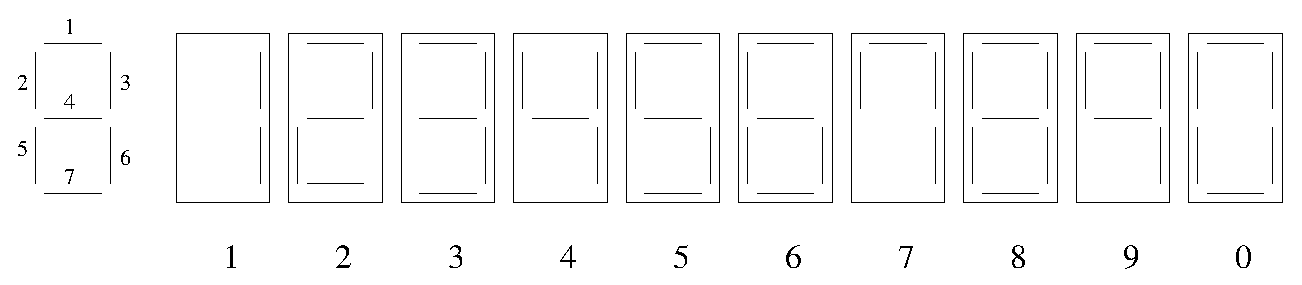
\includegraphics{./FigHw4/Prob4-5}}}
\caption{The numbering of the segments in a 7-segment display.
The patterns of the BCD digits.}
\label{fig:BCD}
\end{figure}

The pattern of LEDs to illuminate for each BCD digit is shown on the 
right-hand side of Figure~\ref{fig:BCD}.  A BCD to 7-segment converter 
has four inputs, $d_3 d_2 d_1 d_0$ and seven outputs $S_7 \ldots S_1$.  
Complete the design using Espresso.  Make sure to include ``Don't cares" 
in the truth table specification. 
\begin{enumerate}
	\item Use Espresso to determine the \SOPmin expression for the outputs 
	$S_7 \ldots S_1$.  Underline product terms that are shared.
	Submit the Espresso source file.

\begin{solution}{
The following is the source file for the BCD to 7-segment converter.

%% \begin{verbatim}
%% # BCD to 7-segment display
%% #
%% .i 4 
%% .o 7  
%% .ilb b3 b2 b1 b0  
%% .ob  s7 s6 s5 s4 s3 s2 s1 
%% 0000 1110111 
%% 0001 0100100 
%% 0010 1011101 
%% 0011 1101101 
%% 0100 0101110 
%% 0101 1101011 
%% 0110 1111011 
%% 0111 0100111 
%% 1000 1111111 
%% 1001 0101111 
%% 101- ------- 
%% 11-- -------  
%% .e  
%% \end{verbatim}

The following is the output from espresso on the 
BCD to 7-segment converter.

%% \begin{verbatim}
%% .i 4 
%% .o 7 
%% .ilb b3 b2 b1 b0 
%% .ob s7 s6 s5 s4 s3 s2 s1 
%% .p 9 
%% --11 0100100 
%% -00- 0100100 
%% -000 1010011 
%% --10 1011000 
%% -100 0101110 
%% -11- 0100011 
%% -101 1101011 
%% -01- 1001101 
%% 1--- 0001011 
%% .e 
%% \end{verbatim}
} \end{solution}

	\item Use Espresso to determine the \POSmin expression for the outputs 
	$S_7 \ldots S_1$.  Underline sum terms that are shared.
	Submit the Espresso source file
\begin{solution} {
The following output was generated by using the same file
as the solution in the previous part; but using the epos
option in espresso.

%% \begin{verbatim}
%% # BCD to 7-segment display 
%% # 
%% .i 4 
%% .o 7 
%% .ilb b3 b2 b1 b0 
%% .ob s7 s6 s5 s4 s3 s2 s1 
%% #.phase 0000000 
%% .p 9 
%% 000- 0001000 
%% -110 0000100 
%% -010 0100010 
%% -101 0010100 
%% 0001 1010011 
%% -011 0010010 
%% -100 1010001 
%% 1--1 1010000 
%% -111 1011000 
%% .e 
%% \end{verbatim}

Remember that these are the negation of the output variables, hence
we have to use DeMorgan's to put them into \POSmin form.  
Symbolically we have:
%% \begin{verbatim}
s7=(b3+b2+b1+b0')(b2'+b1+b0)(b3'+b0')(b2'+b1'+b0'); \\
s6=(b2+b1'+b0); \\
s5=(b2'+b1+b0')(b3+b2+b1+b0')(b2+b1+b0')(b2'+b1+b0)(b3'+b0')(b2'+b1'+b0'); \\
s4=(b3+b2+b1)(b2'+b1'+b0'); \\
s3=(b2'+b1'+b0)(b2'+b1+b0'); \\
s2=(b2+b1'+b0)(b3+b2+b1+b0')(b2+b1'+b0'); \\
s1=(b3+b2+b1+b0')(b2'+b1+b0); \\
%% \end{verbatim}
}\end{solution}
\end{enumerate}

\item {\bf (10 pts.)} Build a box which has one 4-bit input called A and  
one 4-bit output called T. The output T is the 2's-complement value
of the input A.  Use the bit slice paradigm to solve this
problem.  That is, create a building block for one bit of the problem 
then string four of them together to solve the problem.
For the problem at hand this can be done as follows:
\begin{enumerate}
	\item Start at the LSB of A.
        \item If this is the first, least significant, 1, flip all bits 
		to the left.
        \item If this is not the first 1, leave the bit alone.
        \item Move one bit to the left.
        \item Goto Step b.
\end{enumerate}
A bit-slice should communicate whether there has been a 1 to the right,
to the more significant bit.  Submit:
\begin{itemize}
	\item How the above "algorithm" behaves when presented with
        the inputs A=1100
        \item The truth table for one bit slice
        \item \SOPmin expression and circuit diagram for a bit slice.
        \item The organization of four bit slices to solve the problem
\end{itemize}

\begin{solution}{
	The key to the begin solution  is to figure out the structure
	of the begin solution  and then give meaning to the signals involved.
	The problem will be sliced into four bit-slices; each handled
	but its own complement box.  Thus, there will be four complement
	box in the begin solution.  Each box will have 2 inputs, one being
	a bit of A and the other being a "carry in" from the less
	significant less, immediately to the right.  Each box
	will have two bits of output, a bit of T and a "carry out".
	The carry bits (both into and out of a box will convey
	information regarding the rightmost 1 in the number A.

	If the carry in is equal 1 then there is a one to the right. 
	If the carry in is equal 0 then there is not a one to the right. 
	The truth table for a box is then

	\begin{table}
	\begin{tabular}{l|l||l|l|l}
	$A$ & $c_{in}$  & $T$ & $c_{out}$ & comment \\ \hline
	0   & 0   	&   0 & 0    	  & There is no 1 to the right \\ \hline
	0   & 1   	&   1 & 1    	  & There is a 1 to the right, flip A \\ \hline
	1   & 0   	&   1 & 1    	  & There is is no 1 to the right, but we've created one \\ \hline
	1   & 1   	&   0 & 1    	  & There is a 1 to the right, flip A \\ 
	\end{tabular}
	\end{table}

	From this it follows that: \\
	$T=A'c_{in} + A c_{in}'=A \oplus c_{in}$ \\
	$c_{out} = A + c_{in}$
}\end{solution}

\item {\bf (4 pts.)} Build a 7:128 decoder using a minimum number of 
4:16, 2:4 and 1:2 decoders. Describe the wiring of the select lines.
\begin{solution} {

\begin{figure}[ht]
\center{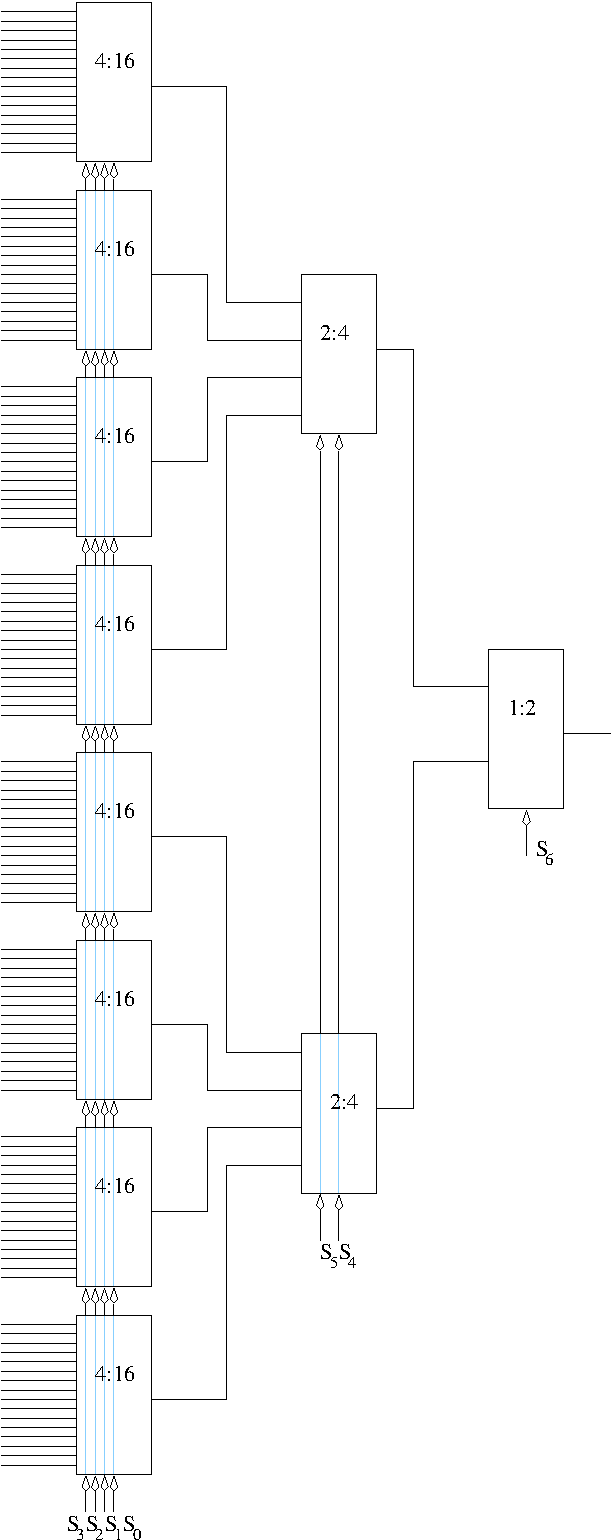
\includegraphics{./FigHw4/Sol4-7}}
\caption{A 7:128 decoder built from 4:16, 2:4 and 1:2 decoders.}
\label{fig:bighwdec}
\end{figure}
} \end{solution}



\item {\bf (4 pts. each)} Design a circuit with two 8-bit inputs $X,Y$, an 
8-bit output $Z$ and a 1-bit input $sel$.  Construct a circuit that yields the 
correct value of $Z$ using only the basic building blocks presented in this 
chapter; do NOT show the internal organization of these building blocks.  If 
a mux is used, denote which input is the $y_0$ and which is $y_1$.  
If a comparator is used denote which input is $X$ and which is $Y$.
Do not use any AND or OR gates; it will tempting in the later problems.
\begin{enumerate}
\item \verb^ if (sel==0) then Z = X else Z = Y ^

\begin{solution}{ 
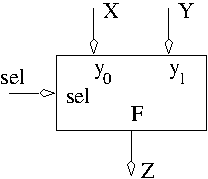
\includegraphics{./FigHw4/Sol4-8a}
} \end{solution}

\item \verb^ if (sel==0) then Z = X+Y else Z = Y ^

\begin{solution}{ 
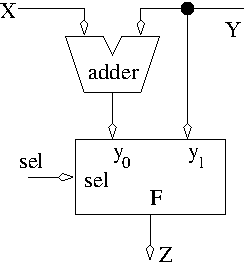
\includegraphics{./FigHw4/Sol4-8b}
} \end{solution}

\item \verb^ if (sel==0) then Z = X+Y else Z = X-Y ^

\begin{solution}{
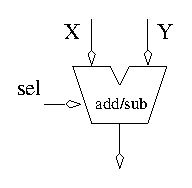
\includegraphics{./FigHw4/Sol4-8c}
} \end{solution}

\item \verb^ if (X==0) then Z = X else Z = Y ^

\begin{solution}{
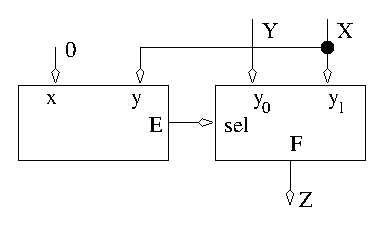
\includegraphics{./FigHw4/Sol4-8d}
} \end{solution}

\item \verb^ if (X==Y) then Z = X-Y else Z = Y ^

\begin{solution}{
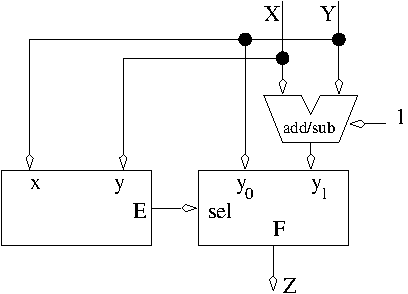
\includegraphics{./FigHw4/Sol4-8e}
} \end{solution}

\item \verb^ if (X==Y) then Z = X+Y else Z = X-Y ^

\begin{solution}{
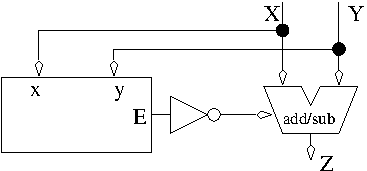
\includegraphics{./FigHw4/Sol4-8f}
} \end{solution}

\item \verb^ if (X < Y) then Z = X else Z = Y ^

\begin{solution}{
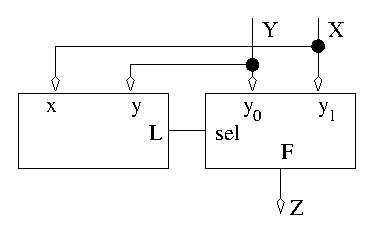
\includegraphics{./FigHw4/Sol4-8g}
} \end{solution}

\item \verb^ if (X <= Y) then Z = X else Z = Y ^

\begin{solution}{
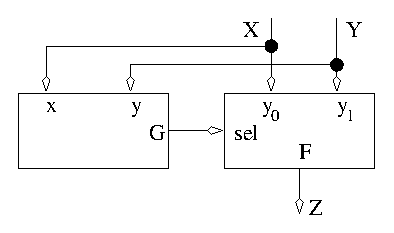
\includegraphics{./FigHw4/Sol4-8h}
} \end{solution}

\item \verb^ if (X > Y) then Z = X else Z = Y ^

\begin{solution}{
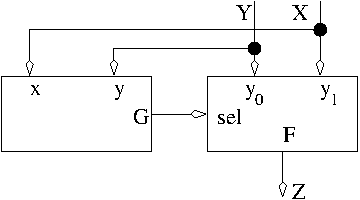
\includegraphics{./FigHw4/Sol4-8i}
} \end{solution}

\item \verb^ if (X > Y) then Z = X+X else Z = Y+Y ^

\begin{solution}{
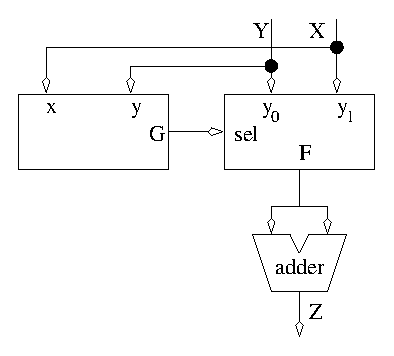
\includegraphics{./FigHw4/Sol4-8j}
} \end{solution}

\end{enumerate}

\item {\bf (10 pts.)} Build a 4-bit priority encoder.

\index{priority encoder}
\begin{tabular}{|l|p{3.5in}|} \hline
Nomenclature:  & N-bit priority encoder                \\ \hline
Data Input:    & N-bit vectored  $D=d_{N-1} \ldots d_1 d_0$  \\ \hline
Data Output:   & $\log_2(N)$-bit vector $Y=y_{log_2(N)} \ldots y_1 y_0$    \\ \hline
Control:       & none					\\ \hline
Status:        & none                                   \\ \hline
Behavior:      & $F = i$ where $i$ is the highest indexed input
			which equals 1.  When all inputs equal
			0, the output is a ``don't care".  \\ \hline
\end{tabular}
\label{page:prior}

The idea is for the outputs to represent (in binary code) the highest
input index which equals 1.  For example, a 4-bit priority encoder
with input $D=1010$ has inputs $d_3=1$ and $d_0=1$.  Of these two
inputs, the index of $d_3$ is greater than the index of $d_0$ so the
output, $F$ is equal to 3, or in binary $11$.  If the input were
$D=0111$ then $F=10$.

\begin{enumerate}
\item Write down the truth table for a 4-bit priority encoder.  Hint, 
the truth table could be structured so that it contains only five rows
by using ``don't cares" on the inputs.

\begin{solution}{
\begin{tabular}{l|l|l|l||l|l}
$d_3$ & $d_2$ & $d_1$ & $d_0$ & $f_1$ & $F_0$ \\ \hline
   0  &    0  &    0  &    0  &    x  &    x  \\ \hline
   0  &    0  &    0  &    1  &    0  &    0  \\ \hline
   0  &    0  &    1  &    x  &    0  &    1  \\ \hline
   0  &    1  &    x  &    x  &    1  &    0  \\ \hline
   1  &    x  &    x  &    x  &    1  &    1  \\
\end{tabular}
} \end{solution}

\item An \SOPmin realization of the circuit.
\begin{solution}{
$f_1 = d_3 + d_2$ \\
$f_0 = d_3 + d_2'd_1$
}\end{solution}
\end{enumerate}

\item {\bf (10 pts.)} Build a 4-bit saturation adder.  A
saturation adder performs normal 4-bit addition when the 
resulting sum is less than 15.  If the sum is
greater than 15, the saturation adders outputs 15.  The
following table summarizes.

\index{saturation adder}
\label{page:saturation}
\begin{tabular}{|l|p{3.5in}|} \hline
Nomenclature:  & 4-bit saturation adder                \\ \hline
Data Input:    & 2, 4-bit vectors \verb+A, B+  \\ \hline
Data Output:   & 4-bit vector \verb+sum+    \\ \hline
Control:       & none                                   \\ \hline
Status:        & none                                   \\ \hline
Behavior:      & 
				\begin{verbatim}
				if (A+B > 15) sum = 15
				else sum = A+B
				\end{verbatim}
		 \\ \hline
\end{tabular}

Submit a schematic showing the basic building blocks, their
data status, and control interconnections.  Show any truth
tables used to build glue logic.

\begin{solution}{
All we need to do is to determine when the sum is greater then
15 and output 15 when it is.  The comparator/mux combo mentioned
several times in the chapter should do the trick.

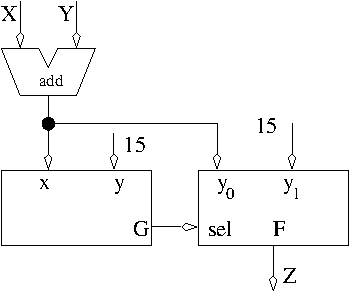
\includegraphics{./FigHw4/Sol4-10}

} \end{solution}

\item {\bf (10 pts.)} Build a mod-6 adder.  The mod-6 adder
takes as input two 3-bit (mod 6) numbers and adds them together
modulus 6.  

\index{modular arithmetic}
\label{page:mod}
Modular arithmetic only operates with a limited portion of the
integers.  The range of numbers is $\{0,1,2, \ldots ,m-1\}$ where 
$m$ is called the {\it modulus}; note there are $m$ different 
integers because counting started at 0.  For example, when working
in mod-6 arithmetic use the integers $\{0,1,2,3,4,5\}$.
To solve any addition problem in modular arithmetic, it is only 
necessary to perform regular addition with the special rule that 
the addition process rolls over from the largest number, $m-1$ to 0
when the result is larger than $m-1$.  For 
example, in mod-6 arithmetic $(5+1) \mod 6 = 0$.  The statement 
``$\mod 6$" is always included in the addition problem to indicate 
to the reader that mod-6 arithmetic is being performed.  Here
are a few more examples to help

\begin{tabular}{l}
$2+3~\mod 6 = 5$ \\
$3+3~\mod 6 = 0$ \\
$4+3~\mod 6 = 1$ \\
$5+5~\mod 6 = 4$ 
\end{tabular}

\index{modular adder}
\label{page:modadder}
\begin{tabular}{|l|p{3.5in}|} \hline
Nomenclature:  & 3-bit mod 6 adder                \\ \hline
Data Input:    & two, 3-bit (mod-6) vectors \verb+A, B+  \\ \hline
Data Output:   & 3-bit (mod-6) vector \verb+sum+    \\ \hline
Control:       & none                                   \\ \hline
Status:        & none                                   \\ \hline
Behavior:      & 
				\begin{verbatim}
				sum = A+B mod 6
				\end{verbatim}
		 \\ \hline
\end{tabular}

Submit a schematic showing the basic building blocks, their
data status, and control interconnections.  Show any truth
tables used to build glue logic.  Be careful that the word
size of the result is handled correctly.

\begin{solution}{
Since the inputs are mod 6 numbers then the inputs can be in the
range [0-5].  Adding two such values will yield a value in the 
range [0-10].  Hence a simple adjustment of the sum when its larger
that 5 is required.

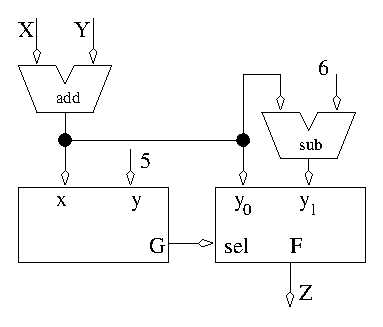
\includegraphics{./FigHw4/Sol4-11}

} \end{solution}

\item {\bf (1pt. each)}Convert the following to 2's-complement 
assuming a word size of eight bits. 
\begin{enumerate}
\item -35 

\begin{solution}{
$35 = 32+2+1 = 100011 = 00100011$, thus $-35=11011101$
} \end{solution}

\item  -128 

\begin{solution}{
This is a special case, see page 10 for more information.
$-128 = 10000000$
} \end{solution}

\item  67 

\begin{solution}{
$67=64+2+1 = 100 0011 = 0100 0011$
} \end{solution}

\item  128 

\begin{solution}{
There are not enough bits to represent this positive number; hence
the 8-bit representation does not exist.
} \end{solution}

\end{enumerate}


\item {\bf (1 pt. each)} Perform the following operations for the given 
2's-complement numbers. Assume a word size of eight bits
in all cases. Indicate where overflow occurs. If there is no overflow, 
convert the result to decimal. 
\begin{enumerate}

\item 01011101 + 00110111 

\begin{solution}{
 01011101 + 00110111 = 10010100  overflow
} \end{solution}

\item 11101011 + 11110001 

\begin{solution}{
 11101011 + 
 11110001 =
 11011100
} \end{solution}

\item 01011101 + 10101011 

\begin{solution}{
 01011101 + 
 10101011 =
 00001000
} \end{solution}

\item 10111011 - 11110001 

\begin{solution}{
 10111011 - 
 11110001 =

 10111011 +
 00001111 =
 11001010
} \end{solution}

\item 01011101 - 00110111 

\begin{solution}{
 01011101 - 
 00110111 =

 01011101 +
 11001001 =
 00100110
} \end{solution}

\item 01011101 - 10101111 

\begin{solution}{
 01011101 - 
 10101111 =

 01011101 +
 01010001 =
 10101110, overflow
} \end{solution}

\end{enumerate}

\item{\bf (5 pts.)} Build a 4-bit bus transceiver.  A bus transceiver
is defined by the following truth table.
                                                                                
\index{bus transceiver}
\label{page:bustranciever}
\begin{tabular}{|l|p{3.5in}|} \hline
Nomenclature:  & N-bit bus transceiver.                    \\ \hline
Data:          & two bidirectional N-bits vectors $X=x_{N-1} \ldots x_1 x_0$.                                                                                 
                        $Y=y_{N-1} \ldots y_1 y_0$.          \\ \hline
Control:       & 1-bit $F$ and $R$             \\ \hline
Status:        & none                                   \\ \hline
Behavior:      &
                        \begin{tabular}{c|c|c|c||c}
                        F  & R  & X & Y & comment \\ \hline
                        0  & 0  & Z & Z & X and Y tristate \\ \hline
                        0  & 1  & Y & Y & X = Y  \\ \hline
                        1  & 0  & X & X & Y = X  \\ \hline
                        1  & 1  & x & x & never applied \\
                        \end{tabular} \\ \hline
\end{tabular}
\label{page:bus}
\\ \\
Flow is determined by the $F$ and $R$ signals denoting forward and reverse
respectively.  When $F=1$, data flows from $X$ to $Y$.  In this case,
$X$ is acting like and input and $Y$ is acting like an output.  When
$R=1$, data flows from the $Y$ input to the $X$ output.  This design
relies heavily on tristate buffers.
                                                                                
\begin{solution} {
\begin{figure}[ht]
\center{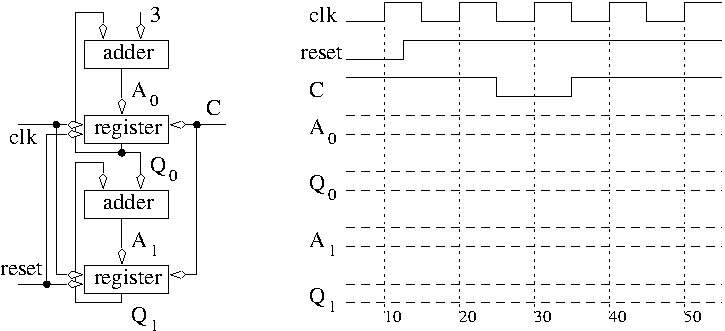
\includegraphics{./FigHw4/Prob4-16}}
\end{figure}
} \end{solution}
                                                                                
\item{\bf (3 pts.)} Build a 2:1 mux using some tristate buffers and an inverter.                                                                                
\item{\bf (3 pts.)} Build a 4:1 mux using some tristate buffers and two inverters.
                                                                                
\begin{solution} {
\begin{figure}[ht]
\center{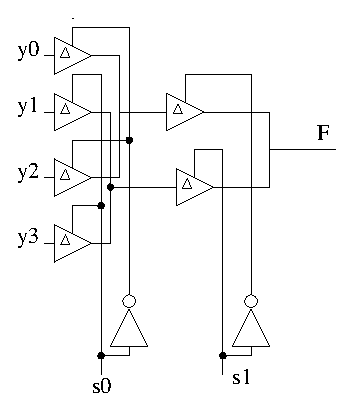
\includegraphics{./FigHw4/Prob4-17}}
\end{figure}
} \end{solution}
                                                                                
\item {\bf (10 pts.)}
\label{page:flipbox}
Build a flip box.  A flip box is defined by the following input,
output, and behavior definition.

\begin{tabular}{|l|p{3.5in}|} \hline
Nomenclature:  & 8-bit flip box.                    \\ \hline
Data Input:    & 8-bit $D=d_7 \ldots d_0$          \\ \hline
Data Output:   & 8-bit $F=f_7 \ldots f_0$          \\ \hline
Control:       & 3-bit $S=s_2 s_1 s_0$            \\ \hline
Status:        & none                                   \\ \hline
Behavior:      & The output is the same as the input except for
		one bit which is inverted.  The index of the inverted
		bit is given by $S$. \\ \hline
\end{tabular}

The flip box takes the 8-bit data input, flips a single bit identified
by $S$, then sends the new 8-bit value to the output.  
For example, if $D=11110000$ and $S=010$ then
$F=11110100$.  If $D=11110000$ and $S=101$ then $F=11010000$.  The solution
should rely heavily on the basic building blocks.

\begin{solution} {
Arrange 8, 2:1 muxes with $d_i$ and $d_i'$ going into the data inputs.
Run the select into a 3:8 decoder and route the data outputs to the 
individual selects of the 2:1 muxes.
} \end{solution}


\item {\bf (10 pts.)}
\label{page:IsScan}
Build a box which recognizes some keyboard scancode.  When a key is 
pressed on a keyboard, the keyboard transmits (among other things) 
an 8-bit scancode of the pressed key.  Each key has its own scancode 
listed in Table~\ref{table:scancodes}.  The relationship between the 
keys and their scancode is not based on ASCII.

\begin{table}
\begin{tabular}{|l|l||l|l||l|l||l|l|} \hline
Key & scancode & Key & scancode & Key & scancode & Key & scancode \\ \hline \hline 
0 & $45_{16}$ & 1 & $16_{16}$ & 2 & $1E_{16}$ & 3 & $26_{16}$ \\ \hline
4 & $25_{16}$ & 5 & $2E_{16}$ & 6 & $36_{16}$ & 7 & $3D_{16}$ \\ \hline
8 & $3E_{16}$ & 9 & $46_{16}$ & A & $1C_{16}$ & B & $32_{16}$ \\ \hline
C & $21_{16}$ & D & $23_{16}$ & E & $24_{16}$ & F & $2B_{16}$ \\ \hline
P & $4D_{16}$ & L & $4B_{16}$ & M & $3A_{16}$ & I & $43_{16}$ \\ \hline
\end{tabular}
\caption{Some keyboard scancodes.}
\label{table:scancodes}
\end{table}

\label{page:scanclass}
\begin{tabular}{|l|p{3.5in}|} \hline
Nomenclature:  & scancode classifier                   \\ \hline
Data Input:    & 8-bit $D=d_7 \ldots d_0$          \\ \hline
Data Output:   & IsP, IsL, IsM, IsI, IsS \\ \hline
Control:       & none             \\ \hline
Status:        & none                                   \\ \hline
Behavior:      & IsP =1 when $D$ is the scan code for the letter ``P".
		 IsL =1 when $D$ is the scan code for the letter ``L".
		 IsM =1 when $D$ is the scan code for the letter ``M".
		 IsI =1 when $D$ is the scan code for the letter ``I".
		 IsS =1 when $D$ is the scan code for the letter ``S".  \\ \hline
\end{tabular}

\item {\bf (10 pts.)}
\label{page:ScanDecode}
Build a box which converts an 8-bit scancode for a hexadecimal
digit into a 4-bit hexadecimal values.

\label{page:scanconv}
\begin{tabular}{|l|p{3.5in}|} \hline
Nomenclature:  & scancode classifier                   \\ \hline
Data Input:    & 8-bit $D=d_7 \ldots d_0$          \\ \hline
Data Output:   & 4-bit $H=h_3h_2h_1h_0$ \\ \hline
Control:       & none             \\ \hline
Status:        & none                                   \\ \hline
Behavior:      & Converts the scancode $D$, representing a the
		key of a hexadecimal character, into its 4-bit 
		value $H$.
		 \\ \hline
\end{tabular}

For example, if $D=25_{16}$, the scancode for the "4" key, then the converter
should output $H=0100_2$.  Assume that the inputs are always
legal hexadecimal scancodes.

\end{enumerate}


%\setcounter{chapter}{5}
%\setcounter{section}{-1}
\chapter{Sequential Circuits}
\begin{enumerate}

\item {\bf (8 pts.)}Determine the state table for the circuit in Figure~\ref{fig:NANDs}.
\begin{figure}[ht]
\center{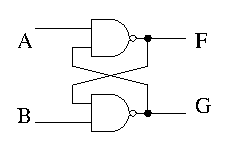
\includegraphics{./FigHw5/Prob5-1}}
\caption{}
\label{fig:NANDs}
\end{figure}


\begin{solution}{
The analysis of the cross-coupled NANDs show in Figure~\ref{fig:nand} is
almost exactly the same as that for the cross coupled NORs.  Start with
the truth table for an NAND gate:

\begin{tabular}{l|l||l}
a & b & (ab)' \\ \hline
0 & 0 & 1 \\ \hline
0 & 1 & 1 \\ \hline
1 & 0 & 1 \\ \hline
1 & 1 & 0 \\ 
\end{tabular}

Observe that the output is 1 whenever
either input is 0.  Now onto the state table for the cross coupled NANDs:

\begin{tabular}{l|l||l|l}
A & B & $F^+$ & $G^+$ \\ \hline
0 & 0 & 1 & 1 \\ \hline
0 & 1 & 1 & 0 \\ \hline
1 & 0 & 0 & 1 \\ \hline
1 & 1 & F & G \\ 
\end{tabular}

For the cross coupled NANDs the output holds when the input $A,B=1,1$ occurs.
In fact if you compare this table to that of the cross coupled NORs, you will
notice that $A,B = S',R'$ and $F,G = Q,Q'$.
} \end{solution}

\item {\bf (8 pts.)} Determine the state table for the circuit 
in Figure~\ref{fig:DLatch}.  Which basic memory element does it act 
like?  Hint, one of the inputs is acting like a clock.  Additional
hint, in order to simplify the analysis, replace a portion of the 
circuit with a component from this chapter.
\begin{figure}[ht]
\center{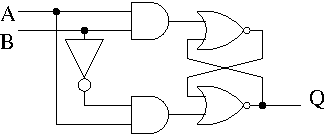
\includegraphics{./FigHw5/Prob5-2}}
\caption{}
\label{fig:DLatch}
\end{figure}

\begin{solution}{
The main idea in this problem is to simplify the cross coupled NOR gates into
an SR latch.  Then use the state table for the SR latch.  This substitution
will simplify the analysis of this circuit.  Since the lower NOR gate is denoted
$A$, call the lower input of the SR latch $R$ and the upper input $S$
(see Figure 5.6).

This yields the following truth table:

\begin{tabular}{l|l|l|l|l||l}
A & B & S & R & comment & $Q^+$ \\ \hline
0 & 0 & 0 & 0 & Hold    & $Q$   \\ \hline
0 & 1 & 0 & 0 & Hold    & $Q$   \\ \hline
1 & 0 & 0 & 1 & Reset   & 0     \\ \hline
1 & 1 & 1 & 0 & Set     & 1     \\ 
\end{tabular}

It is behaving exactly like a D clocked latch, where $A=clk$ and $B=D$.
} \end{solution}

\item {\bf (8 pts.)} Complete the timing diagram for the circuit 
shown in Figure~\ref{fig:DMS}.  Which basic memory element 
does this circuit act like? 

\begin{figure}[ht]
\label{fig:nand}
\center{\scalebox{0.8}{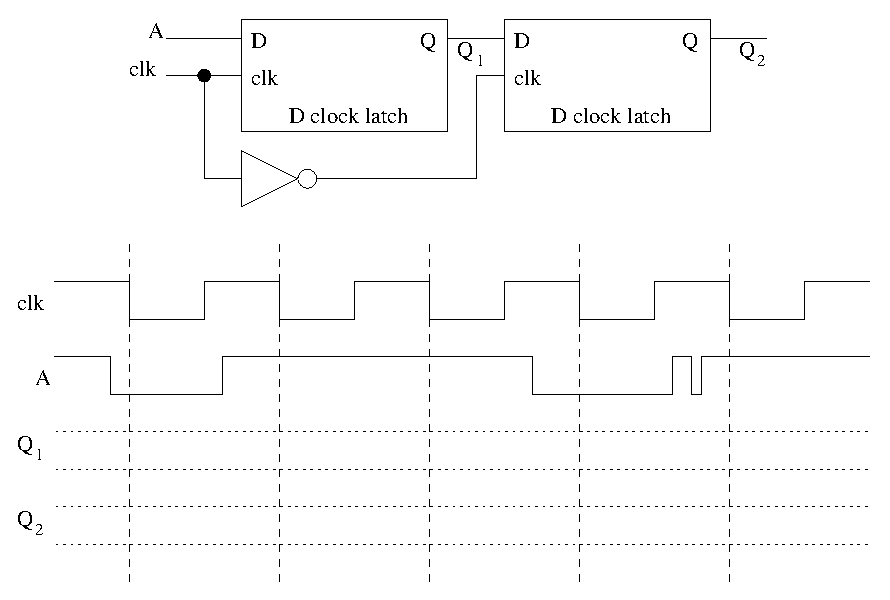
\includegraphics{./FigHw5/Prob5-3}}}
\caption{A 2-stage sequential circuit.}
\label{fig:DMS}
\end{figure}

\item {\bf (15 pts.)} Complete the timing diagram for the basic memory 
elements in Figure~\ref{fig:ExTim}.  The clock cycle is 20 ns. When 
necessary, assume that $Q$ is initialized to 0 and the output settles to 
0 after a period of rapid toggling. 

\begin{figure}[ht]
\center{\scalebox{0.5}{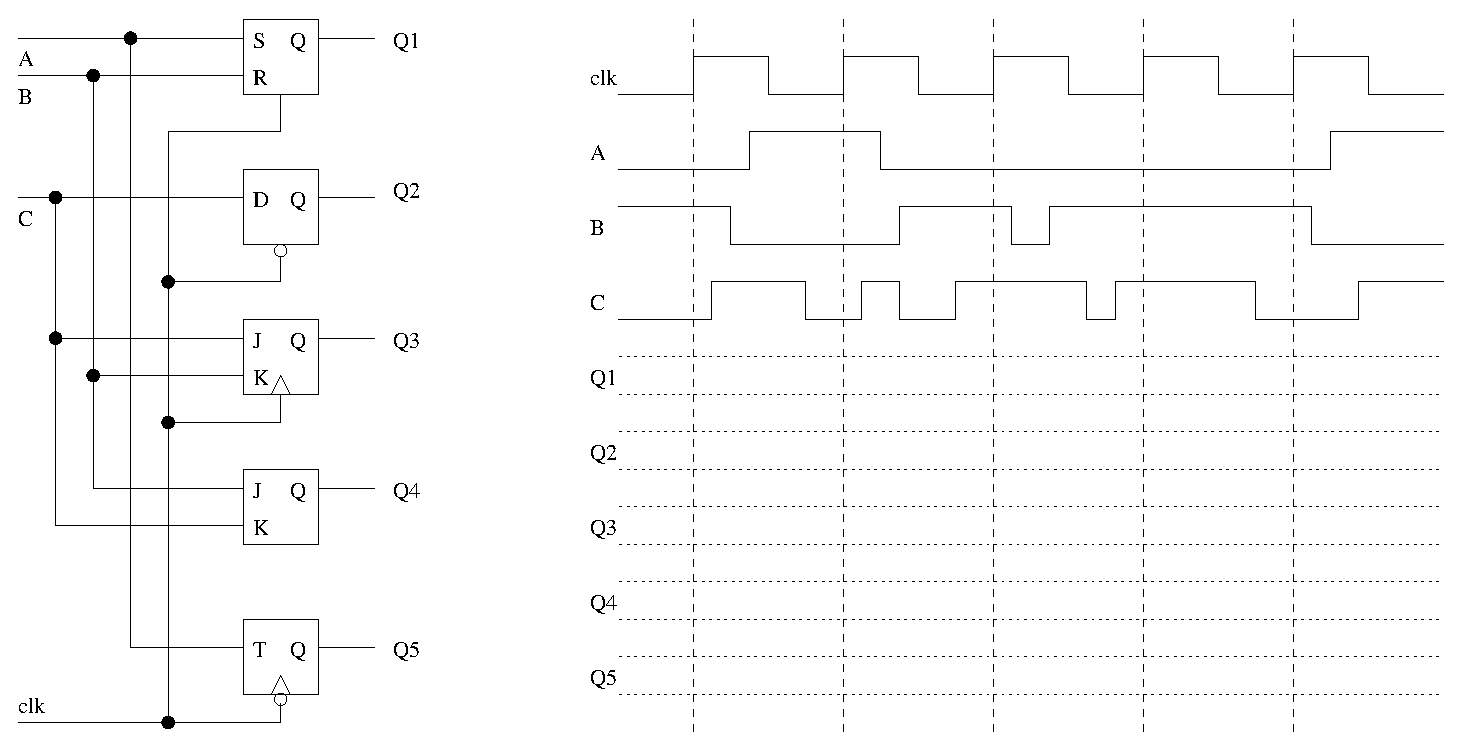
\includegraphics{./FigHw5/Prob5-4}}}
\caption{A variety of basic memory elements and the signals applied to them.}
\label{fig:ExTim}
\end{figure}

\begin{solution}{
\begin{figure}[ht]
\center{\scalebox{0.5}{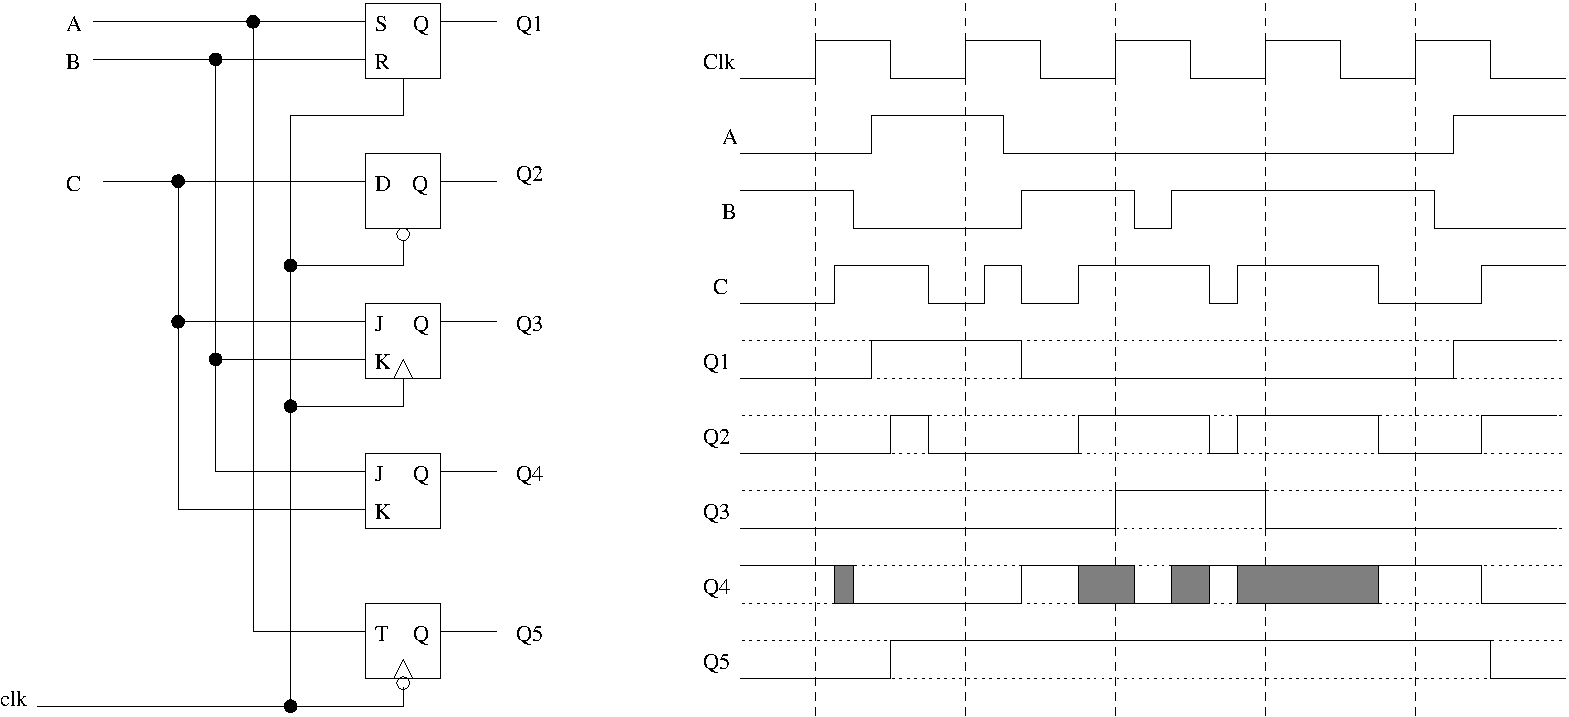
\includegraphics{./FigHw5/Sol5-4}}}
\end{figure}
} \end{solution}


\item {\bf (15 pts.)} Complete the timing diagram for the basic memory elements in 
Figure~\ref{fig:ExTim2}.  The clock cycle is 20 ns. When necessary, 
assume that Q is initialized to 0 and the output settles to 0 after 
a period of rapid toggling. 
\begin{figure}[ht]
\center{\scalebox{0.5}{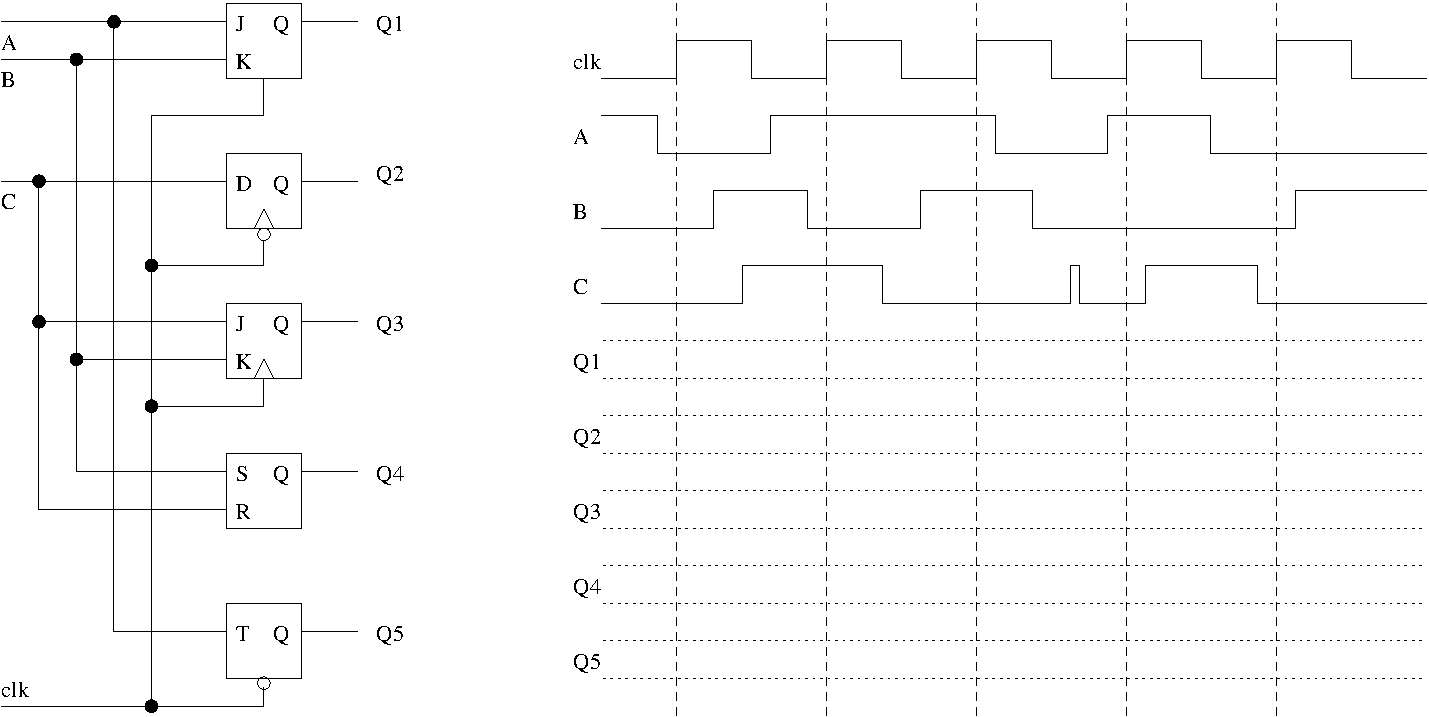
\includegraphics{./FigHw5/Prob5-5}}}
\caption{}
\label{fig:ExTim2}
\end{figure}

\begin{solution}{
\begin{figure}[ht]
\center{\scalebox{0.5}{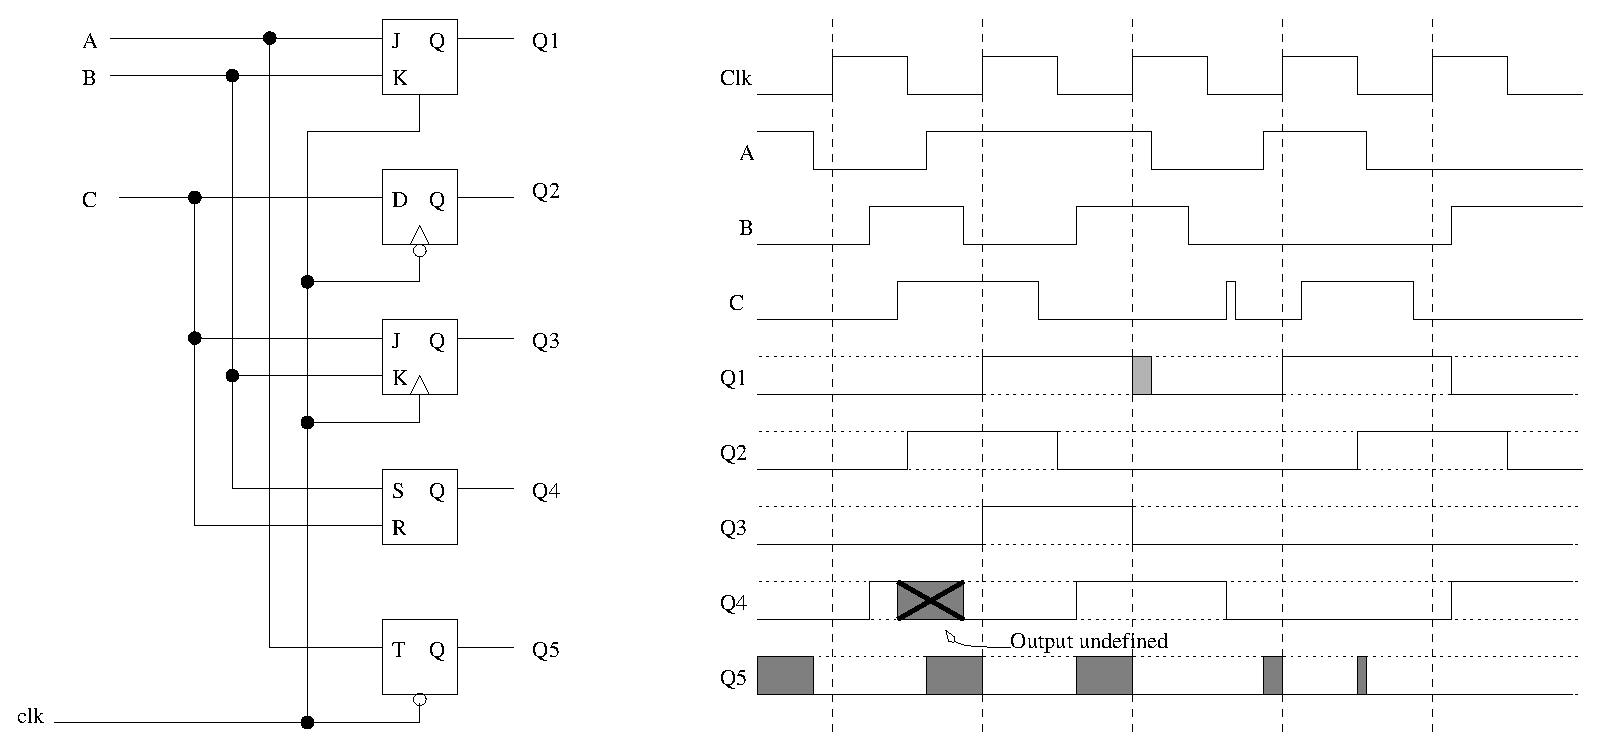
\includegraphics{./FigHw5/Sol5-5}}}
\end{figure}
} \end{solution}


\item {\bf (4 pts.)} Consider the furnace 
controller discussed at the beginning of this chapter.  Determine 
which state the controller should transition into when in a particular state
and given a particular combination of inputs.  
Fill in the eight entries in the following table with the next state
the system should move into.  The next state should be either ON if the 
system should transition (or remain in) the ON state, OFF if the system 
should transition (or remain in) the OFF state, or X if the input 
combination is meaningless. 

\begin{table}[ht]
\center{
\begin{tabular}{c||c|c|c|c}
Current State $\bs T_{hi} T_{low}$& 00	& 01	& 11	& 10	\\ \hline \hline
	ON			&	&	&	&	\\ \hline
	OFF			&	&	&	&	\\ 
\end{tabular}
}
\end{table}
 
\item {\bf (8 pts.)} Derive the next state equations for each 
type (D, T, SR, and JK) of basic memory element.  The next state equation 
is a symbolic equation describing the next state ($Q^+$) 
as a function of the inputs (D,T,SR, or JK) and state ($Q$).
In order to determine the next state equations for a
a JK memory element, build a 3-variable Kmap with 
$Q$, $J$, and $K$ as the inputs.  The entries in the Kmap should 
be $Q^+$.  Solving this Kmap will yield the next state equation.
Show all work for full credit.

\item {\bf (16 pts.)} Derive the transition list for each
type (D, T, JK, and SR) of basic memory element.  A transition 
list describes the input(s) necessary to elicit a particular 
change in state.  For example, imagine that a D flip flop output
is currently in the 0 state and it needs to transition to 
the 1 state after the clock edge.  In other words, $Q=0$ and 
$Q^+ = 1$.  What input would have to be provided on the
$D$ input to make this happen?  Clearly, $D=1$.  This entry
is filled in Table~\ref{table:tl}.

Hint, the Kmaps used to determine the next state equations
will help in visualizing all the conditions which elicit 
a particular change of input.  Complete the transition list 
for all four memory types.  For full credit, show how the
entries in the transition list are determined.

\begin{table}[ht]
\center{
\begin{tabular}{cccc}

\begin{tabular}{c||c}
$Q \rightarrow Q^+$	&	D		\\ \hline \hline
$0 \rightarrow 0$		&		\\ \hline
$0 \rightarrow 1$		&	1	\\ \hline
$1 \rightarrow 0$		&		\\ \hline
$1 \rightarrow 1$		&		\\ 
\end{tabular}

&

\begin{tabular}{c||c}
$Q \rightarrow Q^+$	&	T		\\ \hline \hline
$0 \rightarrow 0$		&		\\ \hline
$0 \rightarrow 1$		&		\\ \hline
$1 \rightarrow 0$		&		\\ \hline
$1 \rightarrow 1$		&		\\ 
\end{tabular}

&

\begin{tabular}{c||c|c}
$Q \rightarrow Q^+$	&	J	&	K		\\ \hline \hline
$0 \rightarrow 0$		&		&		\\ \hline
$0 \rightarrow 1$		&		&		\\ \hline
$1 \rightarrow 0$		&		&		\\ \hline
$1 \rightarrow 1$		&		&		\\ 
\end{tabular}

&

\begin{tabular}{c||c|c}
$Q \rightarrow Q^+$	&	S	&	R		\\ \hline \hline
$0 \rightarrow 0$		&		&		\\ \hline
$0 \rightarrow 1$		&		&		\\ \hline
$1 \rightarrow 0$		&		&		\\ \hline
$1 \rightarrow 1$		&		&		\\ 
\end{tabular}

\\
\end{tabular}
}
\caption{The transition lists for the four types of basic memory elements.}
\label{table:tl}
\end{table}


\end{enumerate}


%\setcounter{chapter}{6}
%\setcounter{section}{-1}
\chapter{Sequential Building Blocks}
\begin{enumerate}
\item {\bf (8 points)} Build a 4-bit universal shift register in
Table~\ref{table:uni} using D flip-flops and 8:1 multiplexers.

\begin{table}
\begin{tabular}{c|c|c||c}
S2 & S1 & S0 & Operation \\ \hline
0  &  0 &  0 & Hold \\ \hline
0  &  0 &  1 & Load \\ \hline
0  &  1 &  0 & ASR  \\ \hline
0  &  1 &  1 & ASL  \\ \hline
1  &  0 &  0 & LSR  \\ \hline
1  &  0 &  1 & LSL  \\ \hline
1  &  1 &  0 & CSR  \\ \hline
1  &  1 &  1 & CSL  \\ 
\end{tabular}
\caption{The truth table for a universal shift register.}
\label{table:uni}
\end{table}

\begin{solution}{
\begin{figure}[ht]
\center{
\includegraphics{./FigHw6/Prob6-1}}
\end{figure}
}\end{solution}

\item {\bf (8 pts.)} Use a counter and a comparator
to implement the following circuits.

\begin{enumerate}
\item Show how to modify the counter (by adding some external logic)
to implement a mod-10 counter.  A mod-10 counter counts from 0 to
9 and then goes back to 0.  It spends one full clock cycle on each
of these count values.

\begin{solution}{
Our mod 10 counter will have 1 data input, representing
the state of the least significant counter.  Call this input
Nine In.  Nine In equals 1 when the less significant counters
output equals 9, otherwise Nine In equals 0.  Our mod 10 counter
will have four bits of output representing the current count value.
The mod 10 counter will also have a Nine Out output which will
equal 1 when our current count value equals 9, otherwise
Nine Out equals 0.  Let the constant value 9 be sent to the Y
input of the comparator and the 4-bit register (Q) sent to the X
input.  When Q<9 the comparator outputs G=0, L=1, E=0.  When
Q=0 then the comparator outputs G=0, L=0, E=1.  Hence by running
the E output of the comparator to the select input of the mux,
the Q+1 will be sent to the register input when Q<9.  Notice
that the register will only latch a new value (Q+1 or 0) when
the less significant counter has rolled over.

\begin{figure}[ht]
\center{
\includegraphics{./FigHw6/Prob6-2}}
\end{figure}

}\end{solution}

\item Use four mod-10 counters to build a 4-digit decimal counter which 
counts up from 0 to 9999.  Draw a schematic for the 4-digit decimal 
counter. 
\begin{solution} {
Just ripple four of the above counter head to tail via Nine In and Nine
Out.  Set the Nine In input of the least significant counter to 1.
} \end{solution}

\end{enumerate}


\item {\bf (8 pts.)} Design a circuit which contains three 8-bit 
registers X,Y,Z.  The behavior of the circuit is determined by the statement:
\begin{verbatim}
if (X > Y) then Z = X+X else Z = Y+Y
\end{verbatim}
The registers are preloaded with values in them.
Submit a circuit diagram showing the building blocks uses,
their interconnections and any miscellaneous logic required to make
them operate together.
\begin{solution} {
\begin{figure}[ht]
\center{
\includegraphics{./FigHw6/Prob6-3}}
\end{figure}
} \end{solution}


\item {\bf (8 pts.)} Design a circuit which contains three registers X,Y,Z.
The behavior of the circuit is determined by the statements:
\begin{verbatim}
1. while (X > 0) {
2.     Z = Z+Y;
3.     X = X-1;
4. } 
\end{verbatim}
The registers are preloaded with values in them.
Submit a circuit diagram showing the building blocks used,
their interconnections and any miscellaneous logic required to make
them operate together.  The design should use an adder and an
adder subtractor plus some other building blocks.  Hint, use
the enable inputs of the registers to control when they
latch information.

\begin{solution} {
\begin{figure}[ht]
\center{
\includegraphics{./FigHw6/Prob6-4}}
\end{figure}
} \end{solution}

\item {\bf (8 pts.)} Given three 32-bit registers A,B,PC, design a circuit
which adds PC and A (putting the result back into PC) when A is equal
to B.  Otherwise, add 1 to PC.  The contents of A and B
are to remain unchanged.

\begin{solution} {
\begin{figure}[ht]
\center{
\includegraphics{./FigHw6/Prob6-5}}
\end{figure}
} \end{solution}

\item {\bf (8 pts.)} Build a circuit that performs the following: 
\begin{verbatim}
    for(i=0; i<100; i++) 
        total = total + i;
\end{verbatim}
Use the counter described in this chapter for the $i$ variable; 
assume that the counter is initialized to 0. \verb^total^ is stored 
in a register and its initialized to 0.  Use a comparator to shut 
down the counter and put the register in hold when the count value 
reaches a critical value. Until this critical value is 
reached the comparator should allow the counter to count and the 
register to load.  

\begin{solution} {
Note that the counter really needs only one of two control settings
00 for holding and 10 for counting up.  Thus, the LSB of the counters
control input can be hardwired to 0.  Its the MSB of the counters control
that needs controlled by the comparator.  Since the counter is in the
range of 0-100, the counter has a 7-bit output.  It is an interesting exercise to
determine the number of bits required for the adder's output so that it 
does not overflow during the computation.  The figure below shows that
13 bits are required (the upper six bits of the counter's output are padded
with 0's so that the counters output can be feed into the adder).

\begin{figure}[ht]
\center{
\includegraphics{./FigHw6/Prob6-6}}
\end{figure}
} \end{solution}


\item{\bf (8 pts.)} Build a circuit that performs the following: 
\begin{verbatim}
    for(i=0; i<100; i++) 
        total = total + 1;
\end{verbatim}

\begin{solution} {
\begin{figure}[ht]
\center{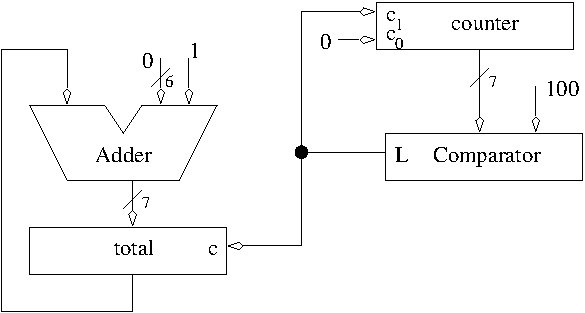
\includegraphics{./FigHw6/Prob6-7}}
\end{figure}
} \end{solution}


\item{\bf (8 pts.)} Design a circuit that can shift (circular 
to the right) the contents of register X by an amount given in 
register Y. X is stored in the circular shift register described 
in this chapter. The solution will require a comparator and a
counter.
\begin{solution} {
\begin{figure}[ht]
\center{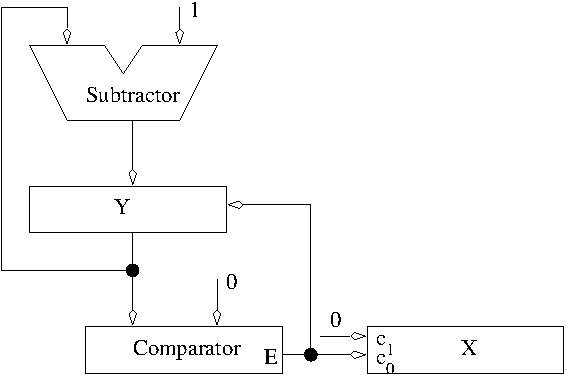
\includegraphics{./FigHw6/Prob6-8}}
\end{figure}
} \end{solution}


\item{\bf (8 pts.)} Assume a 32kx8 RAM is full of data. Show 
the hardware required to realize the following algorithm. 
\begin{verbatim}
    for(i=0; i<32767; i++)
        total = total + M[i];
\end{verbatim}

Where \verb+M[i]+ is the 8-bit word stored at address \verb^i^. 
Assume the total register is initialized to 0. The $i$ variable should 
be the output of a counter. Use a comparator to shut down the counter 
and to put the register in hold when the count value reaches a critical 
value.  
\begin{solution} {
\begin{figure}[ht]
\center{
\includegraphics{./FigHw6/Prob6-9}}
\end{figure}
} \end{solution}


\item{\bf (8 pts.)} Show how to initialize a 32kx8 RAM in the following manner. 
\begin{verbatim}
    for(i=0; i<32767; i++) 
        M[i] = i mod 256;
\end{verbatim}

Where the ``i mod 256" statement means store the least significant 
eight bits of the $i$ variable into the RAM. 

\begin{solution} {
\begin{figure}[ht]
\center{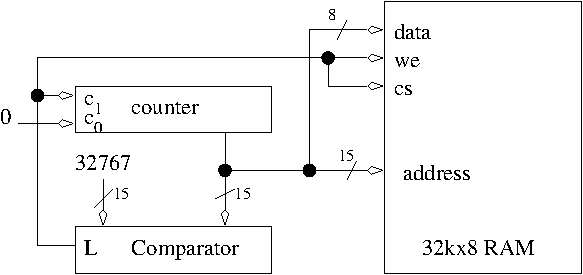
\includegraphics{./FigHw6/Prob6-10}}
\end{figure}
}\end{solution}

\item{\bf (5 pts.)} Complete the timing diagram in Figure~\ref{fig:hwshift}
\label{item:shifter}
for a 4-bit arithmetic shift register.  Use the control setting from the
truth table on page~\pageref{page:shi}.
\begin{figure}[ht]
\center{
\includegraphics{./FigHw6/Prob6-14}}
\caption{The timing diagram for a 4-bit arithmetic shift register in 
Problem~\ref{item:shifter}.}
\label{fig:hwshift}
\end{figure}

\begin{solution} {
\begin{figure}[ht]
\center{
\includegraphics{./FigHw6/Prob6-13}}
\end{figure}
} \end{solution}


\item{\bf (5 pts.)} Complete the timing diagram in Figure~\ref{fig:hwcount}
\label{item:counter}
for a 4-bit counter.  Use the control setting from the truth table on 
page~\pageref{page:counter}.
\begin{figure}[ht]
\center{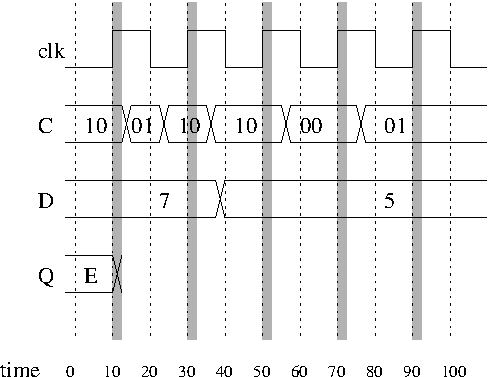
\includegraphics{./FigHw6/Prob6-15}}
\caption{The timing diagram for a 4-bit counter in 
Problem~\ref{item:counter}.}
\label{fig:hwcount}
\end{figure}

\begin{solution} {
\begin{figure}[ht]
\center{
\includegraphics{./FigHw6/Prob6-14}}
\end{figure}
} \end{solution}


\item{\bf (5 pts.)} Complete the timing waveforms for $A_1, A_0, Q_1, Q_0$
\label{item:cascade}
based on the circuit diagram shown in Figure~\ref{fig:cascade}.  Use the truth 
table on page~\pageref{page:reg} for the register. Put the decimal 
representation of the signals in the timing diagram (like the timing 
diagram in Figure~\ref{fig:comb1}).
\begin{figure}[ht]
\center{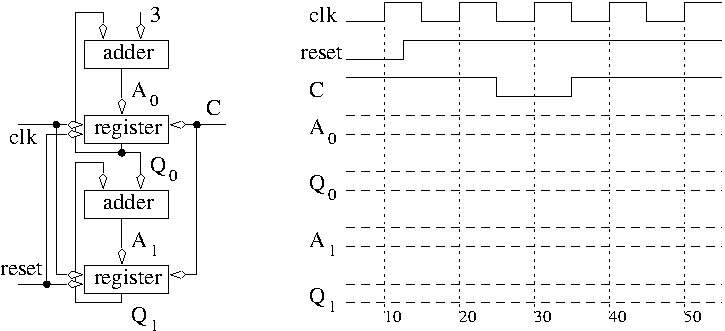
\includegraphics{./FigHw6/Prob6-16}}
\caption{The circuit diagram and incomplete timing diagram for 
Problem~\ref{item:cascade}.}
\label{fig:cascade}
\end{figure}

\begin{solution} {
\begin{figure}[ht]
\center{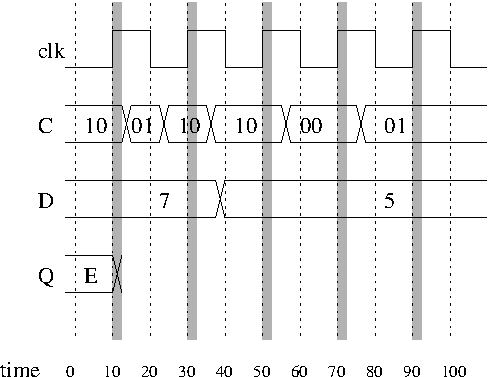
\includegraphics{./FigHw6/Prob6-15}}
\end{figure}
} \end{solution}

\item{\bf (4 pts.)} The circuit shown in Figure~\ref{fig:fib} generates a
Fibonacci sequence, a sequence starting with 1,1,2,3...  The next number in
the sequence is the sum of the preceding two numbers.  Complete the 
timing diagram, assuming the circuit starts with the values shown.
Identify the signal which generates a complete Fibonacci sequence.

\begin{figure}[ht]
\center{\includegraphics{./FigHw6/fib}}
\caption{A circuit which generates a Fibonacci sequence.}
\label{fig:fib}
\end{figure}

\end{enumerate}


%\setcounter{chapter}{7}
%\setcounter{section}{-1}
\chapter{Finite State Machines}
\begin{enumerate}
\item A finite state machine has been implemented with four
flip-flops, two inputs and three outputs. 
	\begin{enumerate}
	\item What are the minimum and maximum number of states in the diagram?
\begin{solution}{
Since there are three flip flops we can have a maximum of 8 states.  The minimum
number of states is a bit tricky.  A practical answer is 5, because if you
had fewer states you would use fewer flip flops.  However, the question
asks for a minimum, in which case you could have 1 state.  Note, that a
1 state FSM would only generate a single output and hence would not be a
very interesting circuit.
}\end{solution}
	\item What are the minimum and maximum number of transition arrows 
		starting at a particular state?
\begin{solution}{
These values are the same.  Since there are two bits of input there are four
different inputs that can be applied at each state.  Thus, four arrows must
leave each state.
}\end{solution}
	\item What are the minimum and maximum number of transition arrows 
		ending in a particular state?
\begin{solution}{
In a typical design your systems will have a reset state, it normal for such
states to have NO input arcs.  You only visit them when the power is turned on.
This is the minimum number of arcs that can terminate at a state.  On the
other hand, I could image a machine where   transition arc points to a
particular state (not a very interesting FSM).  Hence all 32 arcs could point
to a single state.
}\end{solution}
	\item What are the minimum and maximum number of different binary patterns
		that are displayed on the outputs? 
\begin{solution}{
this is a tricky question, you need to determine which of the inputs and outputs
constrains the number of distinct patterns on the output.  You should consult
figure 7.1 for some guidance.  There are three bits of output which have the possibility
of generating 8 different outputs.  There are a total of six bits of input to the
combinational logic box, more than enough to cope with the 8 different output.  On
the other end of the scale, I can imagine a FSM which only produces a single output,
it would however, not be very interesting.
}\end{solution}
	\end{enumerate}


\item {\bf (20 points)}
The state assignment for a FSM influences the amount of
combinational logic required in the realization.  In the following
problem this phenomena is investigated.  Determine the MIEs 
for the following state table using
both the state assignments.

\begin{tabular}{lll}
State Table & State Assignment 1 & State Assignment 2  \\
\begin{tabular}{c|c|c}
CS x & 0    & 1    \\ \hline
A    & A,0  & B,0  \\ \hline
B    & C,1  & F,1  \\ \hline
C    & D,0  & C,0  \\ \hline
D    & A,1  & H,1  \\ \hline
E    & F,1  & E,1  \\ \hline
F    & G,0  & F,0  \\ \hline
G    & G,1  & C,1  \\ \hline
H    & D,1  & E,1  \\ 
\end{tabular}
& 
\begin{tabular}{c||c|c|c}
State & $Q_2$ & $Q_1$ & $Q_0$ \\ \hline
A     & 0     & 0     & 0     \\ \hline
B     & 0     & 0     & 1     \\ \hline
C     & 0     & 1     & 1     \\ \hline
D     & 0     & 1     & 0     \\ \hline
E     & 1     & 0     & 0     \\ \hline
F     & 1     & 0     & 1     \\ \hline
G     & 1     & 1     & 1     \\ \hline
H     & 1     & 1     & 0     \\ 
\end{tabular}
&
\begin{tabular}{c||c|c|c}
State & $Q_2$ & $Q_1$ & $Q_0$ \\ \hline
A     & 0     & 0     & 0     \\ \hline
B     & 1     & 1     & 1     \\ \hline
C     & 0     & 0     & 1     \\ \hline
D     & 1     & 1     & 0     \\ \hline
E     & 1     & 0     & 1     \\ \hline
F     & 0     & 1     & 1     \\ \hline
G     & 1     & 0     & 0     \\ \hline
H     & 0     & 1     & 0     \\ 
\end{tabular}
\end{tabular}

After obtaining the MIEs for both realizations, determine the cost 
of each solution according to the following formula: 
$C(FSM) = A + O + 6*F$.  Where $C(FSM)$ denotes
the cost of the FSM, 
$A$ is the cost of the AND gates,  
$O$ is the cost of the OR gates, and 
$F$ is the number of flip flops.  
The cost of an AND gate is equal to the number of inputs to the 
AND gate.  Likewise the cost of an OR gate is equal to the number
of inputs.  NOT gates are free. For example, the circuit 
$A'B + ABC'$ costs $2+3+2=7$.  

Submit:
\begin{enumerate}
\item Shared steps of the design process.
\item Derive the MIEs for each of the two realizations.
\begin{solution}{

State Assignment 1

\begin{tabular}{l|l|l|l|l}
$Q_2 Q_1 \ Q_0 x$  & 00 & 01  & 11 & 10 \\ \hline
00  & 000,0 & 001,0 & 101,1 & 011,1  \\ \hline
01  & 000,1 & 110,1 & 011,0 & 010,0  \\ \hline
11  & 010,1 & 100,1 & 011,0 & 111,1  \\ \hline
10  & 101,1 & 100,1 & 101,0 & 111,0  \\ 
\end{tabular}

$D_2 = Q_1Q_0'X + Q_1'Q_0X + Q_2Q_0X' + Q_2Q_1'$		\\
$D_1 = Q_2Q_1X' + Q_2'Q_1X + Q_1Q_0 + Q_0X'$			\\ 
$D_0 = Q_2Q_1'X' + Q_2'Q_1'X + Q_1'Q_0 + Q_2Q_0 + Q_0X$ 	\\    
$Z   = Q_2'Q_1'Q_0 + Q_1Q_0' + Q_2Q_0' + Q_2Q_1$		\\ 

State Assignment 2

\begin{tabular}{l|l|l|l|l}
$Q_2 Q_1 \ Q_0 x$  & 00 & 01  & 11 & 10 \\ \hline
00  & 000,0 & 111,0 & 001,0 & 110,0  \\ \hline
01  & 110,1 & 101,1 & 011,0 & 100,0  \\ \hline
11  & 000,1 & 010,1 & 011,1 & 001,1  \\ \hline
10  & 100,1 & 001,1 & 101,1 & 011,1  \\ 
\end{tabular} 

$D_2 = Q_2Q_1'Q_0'X' + Q_2Q_1'Q_0X + Q_2'Q_1Q_0' + Q_2'Q_0'X + Q_2'Q_0X'$ \\
$D_1 = Q_2'Q_1Q_0'X' + Q_2'Q_1'Q_0'X + Q_2Q_1X+Q_1Q_0X + Q_1'Q_0X'$\\
$D_0 = Q_1'X + Q_2'X + Q_2Q_0$					\\
$Z   = Q_1Q_0' + Q_2$						\\

}\end{solution}


\item Determine the cost of each of the two realizations.

\begin{solution}{
\begin{tabular}{l|l|l}
	& State Assignment 1	& State Assignment 2 \\ \hline
$D_2$	& 	15		&	22	\\ \hline
$D_1$	&	14		&	22	\\ \hline
$D_0$	&	17		&	9	\\ \hline
$Z$	&	13		&	4	\\ \hline
Total	& 6*3 + 59 = 77 		& 6*3 + 57 = 75	\\ 
\end{tabular}
}\end{solution}
\item Determine the cost of each of the two realizations using Espresso.
\begin{solution}{
Espresso cost 77 for state assignment  1 \\
Espresso cost 75 for state assignment  2
}\end{solution}
\end{enumerate}

\item {\bf (8 pts.)} Realize the FSM in the previous problem using 
a one-hot encoding.  Determine
the MIEs and the cost of the circuit using the same metric.
It is helpful to convert the state table into a state diagram.
\begin{solution}{
\begin{description}
\item $D_A = Q_AX' + Q_DX'$
\item $D_B = Q_AX$
\item $D_C = Q_BX'+Q_CX+Q_GX$
\item $D_D = Q_CX'+Q_HX'$
\item $D_E = Q_EX+Q_HX$
\item $D_F = Q_BX+Q_EX'+Q_FX$
\item $D_G = Q_FX'+Q_GX'$
\item $D_H = Q_DX$
\item $Z   = Q_B + Q_D + Q_E + Q_G + Q_H$
\end{description}

The cost of this solution is 6*8 + 6 + 2 + 9 + 6 + 6 + 9 + 6 + 2 + 5 = 48 + 51 = 99
}\end{solution}

\item {\bf (8 points)}
Enhance the vending machine discussed in this chapter as follows.
Add two buttons for a beverage selection; {\it regular} soda and {\it diet}
soda, see Figure~\ref{fig:Vend}.  This machine will have a change dispenser.  
If the user deposits more than 35\textcent, the circuit should send a signal to
either the {\it nickel change} dispenser or the {\it dime change} dispenser, 
a single bit sent for one clock cycle to a dispenser will yield a single coin.
When the user deposits 35\textcent (or more) the machine gives any change and 
then waits for one of the two buttons to be depressed.  Depending on the 
selection, the circuit should send a signal to either the 
{\it regular dispenser} or
the {\it diet dispenser} mechanism.  The dispenser need only get a signal for
one clock cycle.  After the dispensing, go back to the reset state.
\begin{figure}[ht]
\center{\includegraphics{./FigHw7/Prob7-10}}
\caption{A basic vending machine.}
\label{fig:Vend}
\end{figure}

\begin{solution}{

\begin{figure}[ht]
\center{\includegraphics{./FigHw7/Sol7-9}}
\end{figure}

Note, that in the figure if a input does not appear on
any arc emanating from a state then it is implied that
this input will have no effect on the next state.  Below
are the outputs for each of the states above.

\begin{tabular}{|l||l|l|l|} \hline
\multicolumn{4}{|c|}{outputs from the vending FSM}              \\ \hline \hline
state & nickel change	& diet dispense & regular dispense      \\ \hline
      & 0 give none	& 0 give none	& 0 given none		\\ \hline
      & 1 give nickel	& 1 dispense diet & 1 dispense regular	\\ \hline
      & 		&		&			\\ \hline
0     & 0		& 0		& 0			\\ \hline
5     & 0		& 0		& 0			\\ \hline
10    & 0		& 0		& 0			\\ \hline
15    & 0		& 0		& 0			\\ \hline
20    & 0		& 0		& 0			\\ \hline
25    & 0		& 0		& 0			\\ \hline
30    & 0		& 0		& 0			\\ \hline
35    & 0		& 0		& 0			\\ \hline
40    & 1		& 0		& 0			\\ \hline
d     & 0		& 1		& 0			\\ \hline
r     & 0		& 0		& 1			\\ \hline
\end{tabular}
}\end{solution}



\item {\bf (6 pts.)}
Build a FSM for a car alarm.  The input to the FSM
comes from a tilt sensor.  The tilt-sensor outputs 1 when the 
car has been physically displaced by a preset amount, otherwise the
tilt sensor outputs 0.  The output of the circuit drives an alarm,
when the alarm output equals 1 the alarm sounds, otherwise the alarm
does not sound.  Once the alarm has been set off, it will continue
sounding until a reset input equals 1, at which point the alarm will
stop sounding.

Draw the state diagram and from this determine the MIEs and OEs.


\item {\bf (12 pts.)}
Build a FSM which displays the revolutions per second
(RPS) of a motor.  The output shaft of the motor is attached to 
a sensor whose output pulses to logic 1 every time the motor's shaft
completes a single revolution.  This sensor signal is attached to
a counter.  The behavior of the counter to the pulse input is determined
by a 1-bit control input (coming from the FSM) given by the following 
truth table.

\begin{tabular}{l|l}
control & behavior \\ \hline \hline
0	& reset to 0 \\ \hline
1	& count up \\
\end{tabular}

The counter's output is eight bits wide, representing two BCD digits.  Thus,
the counter's output will go from 19 to 20 when the control input is 1
and there is a pulse on the sensor line.  This 8-bit output from the
counter is sent to the data input of an 8-bit register.  The register's
control input comes from the FSM.  The output of the register is split
into two nybbles (a 4-bit value is called a nybble)
each sent its own BCD to 7-segment converter.  In order to determine
when a second is up, the FSM is fed a reference signal denoted by 
the variable $R$ with a period of exactly 1Hz and a 50\% duty cycle; 
the duty cycle of a square wave is the proportion of time the signal 
spends at logic 1.   That is $R$ is at logic 1 for half a second and 
then at logic 0 for half a second.  The FSM is being supplied with a 
clock signal, $clk$, with a frequency much greater than 1Hz (perhaps 
in the MHz range).  The architecture of the FSM is given in 
the figure below.  

\includegraphics{./FigWork/RPS}

Submit:
\begin{enumerate}
\item Label the arcs of the FSM with R or R' so that the
 circuit operates correctly.
\item Determine the output for each state.  Instead of writing the
output in each state, list the outputs in the following control
word table.

\begin{tabular}{l||l|l}
state	& counter	& register \\ \hline 
	& 0 reset	& 0 hold \\ \hline
	& 1 count up& 1 reset \\ \hline \hline
RefLo	&		&	  \\ \hline
RefHi	&		&	  \\ \hline
Load 	&		&	  \\ \hline
Reset	&		&	  \\ 
\end{tabular}

\item Determine the output equations.
\item Determine the memory input equations assuming a one-hot
encoding of the states.
\end{enumerate}


\item {\bf (12 pts.)}
Build a digital circuit which controls an automatic garage door opener.  
The garage door circuit has three bits of input.  The first input, called 
$button$, comes from a the main control button used to open or close the 
garage door.  When pressed $button=1$ otherwise $button=0$.  The garage 
door rides in a track, at the top and bottom of of which are two 
limit switches.  The top limit switch equals 1 when the garage door 
is all the way up, otherwise its output equals 0.  The bottom limit 
switch equals 1 when the garage door is all the way down, otherwise 
its output equals 0.  The garage door circuit has two bits of output 
called $motor$.  When $motor=01$, the motor moves the door in a downward 
motion, closing the door.  When $motor=10$, the motor moves the door 
upward, opening the garage door.  When $motor=00$, the motor is turned off.

\begin{figure}[ht]
\center{\includegraphics{./FigWork/Door}}
\caption{The garage door and the circuit controlling it.}
\label{fig:hwgarage}
\end{figure}

Construct the FSM assuming a one-hot encoding of the states.
Determine the memory input equations and output equations.


\begin{solution} {

\paragraph{Control unit}
The control unit includes so called wait states.  Waits states are
a result of the fact that the clock running the FSM is usually 
much faster than the physical phenomena being monitored by the FSM.
Unless told otherwise, you can assume that any FSM that you are 
building has a clock which operates on the order of megahertzs.
This means that the resulting FSM can make around 1 million 
state transitions per second.  Clearly, a garage door needs more
than one millionth of a second to open or close.  Consequently, 
the FSM in this problem needs to wait for the door to be opened.
This is done by having the FSM repetitively check the status of the
door via the up or down limit switches.  In addition to waiting 
for the garage door to open and close the FSM must wait for a 
button press.

\begin{figure}[ht]
\center{\includegraphics{./Fig7/GarageFSM}}
\caption{The FSM for the garage door controller.}
\end{figure}

The state diagram for the garage door controller has four states.
In the open and close state, the FSM is waiting for a button push,
while the button is not pressed the door stays open or closed.  As
soon as the button is pressed the door starts to open or close.
It stays in this state until the limit switches tell the FSM that
the door has reached the limit of its travel.

\paragraph{Memory Input Equations}
Since we are building the garage door controller assuming a
one hot encoding of the states, each state will get its own
flip flop.  Each flip flop will output a 1 when the FSM is 
in that state.  The memory input equations for a particular
state are determined by answering, ``how do you get into that 
state?" The four answers to this questions are provided below.

\begin{tabular}{l}
$D_{open} = Q_{open}button' + Q_{opening}up$ \\
$D_{close} = Q_{close}button' + Q_{closing}down$ \\
$D_{opening} = Q_{close}button+ Q_{opening}up'$ \\
$D_{closing}  = Q_{open}button+ Q_{closing}down'$ \\
\end{tabular}


\paragraph{Output Equations}
The outputs for complex FSMs are usually not written inside the
states, rather a separate table is constructed which contains the
output for each state.   Even though this is a simple example
we will construct an output table.

\begin{tabular}{l|l}
State	& motor		\\ \hline
	& 00 stop	\\ \hline
	& 01 down	\\ \hline
	& 10 up		\\ \hline
open    & 00 		\\ \hline
close   & 00		\\ \hline
opening & 10 		\\ \hline
closing & 01 		\\ 
\end{tabular}

Call the outputs $Z_{m1}$ and $Z_{m0}$, for the most and least
significant bits of the output respectively.  Then the outputs
are determined by asking for which states does the output
equal 1?  The answers to this question are shown below.

\begin{tabular}{l}
$Z_{m1} = Q_{opening}$ \\
$Z_{m0} = Q_{closing}$ \\
\end{tabular}

}\end{solution}


\item {\bf (8 pts.)}
Build a digital circuit to control a single traffic light.  The circuit
has three outputs, $Rlight, Ylight$ and $ Glight$.  When
$Rlight=1$ the red light illuminates otherwise the light is off.
The same behavior holds true for $Ylight$ and $Glight$.  In order
to sequence the lights, the circuit has three timers, Rtimer, Gtimer and 
Ytimer.  Each timer controls the length of time that its light should be 
illuminated.  Each timer has one bit of input and one bit of output.  When a 
timer's input is 0, the timer is reset.  When a timer's one bit
input is 1, the timer 
counts down its preset timer interval.  When a timer counts all the way down,
its output goes to 1 and stays there until the timer is reset (by applying
an input of 0).  The state diagram of the circuit is shown in the
figure below.  As shown in this figure the FSM receives input from the 
three timers, while the output of the FSM controls the counters. Complete
the following three tasks.
\includegraphics{./FigWork/Light}

\begin{enumerate}
\item Label the arcs of the FSM with the input values (Rt, Yt or Gt)
needed to make the circuit operate correctly.  

\item Next, determine what the output should be in each
of the states.  Instead of writing the output in each state, the
outputs are organized in a separate table.  In this table, each
row will contain the output associated with a particular state.
Each column in the table will be associated with one bit of the output.

\begin{tabular}{l||l|l|l|l|l|l}
state	& Rlight & Ylight & Glight & Rtimer & Ytimer & Gtimer	\\ \hline 
	& 0 off  & 0 off  & 0 off  & 0 rst  & 0 rst  & 0 rst	\\ \hline
	& 1 on   & 1 on   & 1 on   & 1 run  & 1 run  & 1 run	\\ \hline \hline
R	&	 &	  &	   &	    &	     &		\\ \hline
Y	&	 &	  &	   &	    &	     &		\\ \hline
G	&	 &	  &	   &	    &	     &		\\ 
\end{tabular}

\item Finally, write the memory input equations and output 
equations for the traffic light controller.  In order to write the
memory input equations use the labels on the state transitions from 
the state diagram.   In order to write the output equations 
use the output table.

\begin{tabular}{p{2in}p{2in}}
        \begin{tabular}{l}
        $Q_{red}$= \\
        $Q_{yellow}$= \\
        $Q_{greew}$= \\
        \end{tabular} 
&
        \begin{tabular}{l}
        $Z_{Rlight}$= \\
        $Z_{Ylight}$= \\
        $Z_{Glight}$= \\
        $Z_{Rtimer}$= \\
        $Z_{Ytimer}$= \\
        $Z_{Gtimer}$= \\
        \end{tabular}
\end{tabular}
\end{enumerate}

\item {\bf (16 pts.)}
Build a FSM which make the hexapod robot shown in Figure~\ref{fig:hexapod}
walk forward.

\begin{figure}[ht]
\center{\includegraphics{./FigHw7/Prob7-11}}
\caption{A hexapod walking robot.}
\label{fig:hexapod}
\end{figure}

Each leg of the hexapod robot is moved by two nitinol (Flexinol) wires.  
At rest, nitinol wire is straight.  When 5 volts (logic 1) is applied to 
the wire, it bends in a particular direction.  The two wires making up
a particular leg are positioned so that they move in perpendicular
directions.  One wire moves a leg up or down and the other will move 
the wire forward or backwards.  The table below elaborates.

\begin{tabular}{l|l|l}
wire   & logic 0 & logic 1	\\ \hline
$w_0$  & down	 & up		\\ \hline
$w_1$  & forward & backward	\\ 
\end{tabular}

The hexapod robot walks by moving three legs in unison; see $A$ and
$B$ in Figure~\ref{fig:hexapod}.  The movements of $A$ and $B$ are
coordinated so that, at times, the hexapod is balanced on three legs.
A portion of the walking gait is shown in Figure~\ref{fig:hexgate};
note that in this figure the viewer is looking down at the top of the 
robot which is moving to the right.  The dotted legs are assumed to be in
the air, solid legs are in contact with the ground.

\begin{figure}[ht]
\center{\includegraphics{./FigHw7/Prob7-11b}}
\caption{The walking gait of the hexapod robot.}
\label{fig:hexgate}
\end{figure}

Assume that the legs can move to their correct position in one clock
cycle.  Define each state as a position of the legs in 
Figure~\ref{fig:hexgate}. Draw the state diagram,
and determine the memory input and output equations.

\begin{solution}{

\begin{figure}[ht]
\center{\includegraphics{./FigHw7/Sol7-11}}
\end{figure}

Note that the states have been given numbers to simplify the
description of the states.  Here is a listing of the outputs 
associated with each state:

\begin{tabular}{l|l|l|l|l}
State  & $Aw_1$ & $Aw_0$ & $Bw_1$ & $Bw_0$  \\ \hline
1	& 0	& 0	 & 1	  & 1		\\ \hline
2	& 1	& 0	 & 0	  & 1		\\ \hline
3	& 1	& 1	 & 0	  & 0		\\ \hline
4	& 0	& 1	 & 1	  & 0		\\ 
\end{tabular}

{\bf MIEs and OEs}

\begin{tabular}{ll}
MIEs		&	OEs			\\
$D_1 = D_4$	&	$Z_{Aw_1} = Q_2 + Q_3$	\\
$D_2 = D_1$	&	$Z_{Aw_0} = Q_3 + Q_4$	\\
$D_3 = D_2$	&	$Z_{Bw_1} = Q_1 + Q_4$	\\
$D_4 = D_3$	&	$Z_{Bw_0} = Q_1 + Q_2$	\\
\end{tabular}

}\end{solution}

\item {\bf (12 pts.)}
\label{item:robot}
Build a FSM which makes the simple robot shown in Figure~\ref{fig:Robot}
move along (track) the black line crossing two intersections.
\begin{figure}[ht]
\center{\scalebox{0.8}{\includegraphics{./FigHw7/Prob7-12}}}
\caption{A simple line-tracking robot that must cross two intersections.}
\label{fig:Robot}
\end{figure}

The FSM has two inputs, a left sensor, denoted {\it ls}, and a right 
sensor, denoted {\it rs}.  These two sensors look down at the ground.  
When a sensor sees white, it outputs 0; when it see black, it outputs 1.  
The sensors are spaced far enough apart that they can straddle the black 
line and see white on either side.  The FSM has two outputs, a left
motor, denoted {\it lm} and a right motor, denoted {\it rm}.  A motor
rotates when it is sent a 1 and does not rotate when it is sent a 0.
The FSM should constantly check that the robot is straddling the line.
If it is not the FSM should take corrective action by stopping one of
the wheels.

Submit the state diagram for the FSM,  MIEs and OEs using 
a one-hot encoding of the states.

\begin{solution}{
\begin{figure}[ht]
\center{\includegraphics{./FigHw7/Sol7-11}}
\end{figure}

\begin{tabular}{l|l|l|l}
State & lm		  & rm			\\ \hline
      & 0 stop left wheel & 0 stop right wheel  \\ \hline
      & 1 turn left wheel & 1 turn right wheel  \\ \hline
      &                   &                     \\ \hline \hline
Reset	 & 1		  & 1			\\ \hline
Straight & 1		  & 1			\\ \hline
Left     & 0		  & 1			\\ \hline
Right    & 1		  & 0			\\ \hline
OnLine   & 1		  & 1			\\ \hline
Up	 & 1		  & 1			\\ \hline
Stop	 & 0		  & 0			\\ 
\end{tabular}
} \end{solution} 

\item {\bf (16 pts.)}
Make the robot from Problem \ref{item:robot} cross 63 intersections.
The problem is that the number of states will grow to large to handle
with a FSM by itself.  Additional hardware, in the form of a counter 
and comparator, are added to the FSM to address this problem.

\begin{figure}[ht]
\center{\includegraphics{./FigHw7/Prob7-13}}
\caption{The innards of a intersection counting, line tracking robot.}
\label{fig:linecounter}
\end{figure}

Assume that the counter is reset to 0 when the circuit
is first turned on.  The robot must still track the line, but
must also count up once every time it crosses an intersection.  Remember
the digital circuit shown in Figure~\ref{fig:linecounter} is
operating much faster than the robot is crossing intersections.
The state diagram needs to have wait states while it crosses
the intersection, similar to those
in the DAISY example.  Assume the counter counts up
when the control input is 1 and the clock rises.  When the control
input is 0, then the counter holds its current count value.

Submit the state diagram for the FSM, OEs and MIEs for a one-hot 
encoding of the states.  

\begin{solution} {
\pagebreak
If you encoded 64 line crossing using only a FSM you would have
on the order of 256 states, 4 for each line crossing.  The solution
is to use a counter to keep track of how many lines have been crossed.
The states below explain.

{\bf DP \& CU}

\begin{figure}[ht]
\center{\includegraphics{./FigHw7/Sol7-12}}
\end{figure}

{\bf Control Word}

\begin{tabular}{l|l|l|l}
State & lm		  & rm			& counter \\ \hline
      & 0 stop left wheel & 0 stop right wheel  & 00 hold \\ \hline
      & 1 turn left wheel & 1 turn right wheel  & 01 load \\ \hline
      &                   &                     & 10 count\\ \hline \hline
Reset	 & 1		  & 1			& 01	  \\ \hline
Straight & 1		  & 1			& 00	  \\ \hline
Left     & 0		  & 1			& 00	  \\ \hline
Right    & 1		  & 0			& 00	  \\ \hline
OnLine   & 1		  & 1			& 00	  \\ \hline
Up	 & 1		  & 1			& 10	  \\ \hline
Stop	 & 0		  & 0			& 00	  \\ 
\end{tabular}

One could easily derive the MIEs and OEs for the FSM.
} \end{solution}

\item {\bf (24 pts.)}
Construct a digital circuit to control the operation of a
simple washing machine, see Figure ~\ref{fig:Wash}.
\begin{figure}[ht]
\center{\includegraphics{./FigHw7/Prob7-14}}
\caption{A humble washing machine with a close-up of the start
button and temperature switch.}
\label{fig:Wash}
\end{figure}
To use the simple washing machine set the temperature switch to 
either hot, tepid or cold and then press the start button.
To build a digital circuit to control the washing of clothes
its necessary to understand the washing cycle.  When the start
button is pressed water of the selected temperature pours 
into the washing drum.  The simple washing machine has two 
electronically controlled water valves, the hot valve admits 
hot water into the washing drum and the cold valve admits 
cold water.  Water continues to pour into the drum until it
fills.  There are two water level sensors; the full switch signals when 
the drum is full of water and the empty switch signals when the drum
is empty.  After the drum is full of water the simple washing machine
starts to agitate the clothes.  The simple washing machine has a motor 
controlled by two bits, which agitates (a rapid back and forth motion), 
spins (a rapid rotation in one direction) or does nothing.  After 
agitating for 15 minutes, the agitation cycle stops and
the machine drains its water.  Water leaves the drum through
a drain valve.  When the drum is emptied of water the washing machine enters
the rinse cycle.   The rinse cycle fills the drum with cold
water and agitates for 5 minutes.  The rinse cycle concludes
by draining the water from the drum.
When the drum is emptied of water the washing machine enters
the spin cycle.  This lasts for 5 minutes.  The simple washing machine 
keeps track of time  using a 5 minute timer.   To use the timer 
it must first be reset for one clock cycle.  After being reset the 
timer will count down as long as the timer input is set to run.  
After 5 minutes have elapsed the timer output will go to logic 1 and 
stay there until the timer is reset.  In order to get longer time
intervals, the timer should be reset for another 5 minutes and count 
down again.  When the spin cycle is done, the washing is complete. The 
inputs from the washing machine to the digital circuit have the 
following meaning.

\begin{tabular}{|l|l|l|l|l|} \hline
\multicolumn{5}{|c|}{inputs to the digital circuit}		\\ \hline \hline
start & temperature & empty       & full       & timer out 	\\ \hline	
0 off & 00 hot      & 0 not empty & 0 not full & 0 nothing	\\ \hline 
1 on  & 01 cold     & 1 empty     & 1 full     & 1 5 minutes elapsed 	\\ \hline 
      & 10 tepid    &		  &	       &		\\ \hline
\end{tabular}

The outputs from the digital to the washing machine have the following meaning.
The left most column is explained below.

\begin{tabular}{|l|||l|l|l|l|l|} \hline
\multicolumn{6}{|c|}{outputs from the digital circuit}			\\ \hline \hline
state & hot     & cold    & motor      & timer in   & drain 	\\ \hline
      & 0 close & 0 close & 00 off     & 00 hold    & 0 close	\\ \hline
      & 1 open  & 1 open  & 01 agitate & 01 reset   & 1 open	\\ \hline
      &		&         & 10 spin    & 10 run     &		\\ \hline \hline
{\bf S1}    &	&	  &	       &	    &		\\ \hline
\end{tabular}

Draw the state diagram for the FSM to control the washing machine.  
Label the arcs of the state diagram with the input (or its negation) 
that causes the transition.  Use simple Boolean expressions on these 
arcs, for example (start and hot).
For each state define the output using a table similar to the one above.
For example, if {\bf S1} is a state fill in the bit values for the o
outputs depending on what state {\bf S1} is supposed to do.
Determine the memory input equations and output equations assuming a one-hot 
encoding.

\begin{solution}{
	\begin{enumerate}
	\item No control table (-6)
	\item Disposable washing machine (-1)
	\item No OEs (-5)
	\item start * cold (-2)
	\item no complements on arcs (-2)
	\end{enumerate}
\begin{figure}[ht]
\center{\includegraphics{./FigHw7/Sol7-13}}
\caption{The FSM for a washing machine.}
\end{figure}

\begin{tabular}{|l|||l|l|l|l|l|} \hline
\multicolumn{6}{|c|}{outputs from the digital circuit}			\\ \hline \hline
state & hot     & cold    & motor      & timer in   & drain 	\\ \hline
      & 0 close & 0 close & 00 off     & 00 nothing & 0 close	\\ \hline
      & 1 open  & 1 open  & 01 agitate & 01 reset   & 1 open	\\ \hline
      &		&         & 10 spin    & 10 start   &		\\ \hline 
      &		&         &	       & 11 stop    &		\\ \hline \hline
HOME  &	0	& 0	  & 00	       & 00	    & 0		\\ \hline
COLD  &	0	& 1	  & 00	       & 01	    & 0		\\ \hline
TEPI  &	1	& 1	  & 00	       & 01	    & 0		\\ \hline
HOT   &	1	& 0	  & 00	       & 01	    & 0		\\ \hline
AGIT  &	0	& 0	  & 01	       & 10	    & 0		\\ \hline
ZERO  &	0	& 0	  & 00	       & 01	    & 0		\\ \hline
DRAI  &	0	& 0	  & 00	       & 01	    & 1		\\ \hline
SPIN  &	0	& 0	  & 10	       & 10	    & 0		\\ \hline
\end{tabular}

The memory input equations are a snap.  
\begin{description}
\item $D_{home} = Q_{home}start' + Q_{spin}time $
\item $D_{cold1} = Q_{home}*start*cold $
\item $D_{tepi} =  Q_{home}*start*tepid $
\item $D_{hot} =  Q_{home}*start*hot $
\item $D_{agit1} = Q_{cold1}*fill + Q_{tepid}*fill + Q_{hit}*fill + Q_{agit1}*time' $
\item $D_{zero1} =  Q_{agit1}*time $
\item $D_{agit2} = Q_{zero1}*time + Q_{agit2}*time' $
\item $D_{zero2} = Q_{agit2}*time $
\item $D_{agit3} = Q_{zero2}*time + Q_{agit2}*time' $
\item $D_{drain1} = Q_{agit3}*time + Q_{drain1}*empty' $
\item $D_{cold2} = Q_{drain1}*empty + Q_{cold2}*fill' $
\item $D_{agit4} =  Q_{cold2}*fill + Q_{agit4}*time' $
\item $D_{drain2} = Q_{agit4}*time + Q_{drain2}*empty' $
\item $D_{spin} = Q_{drain2}*empty + Q_{spin}*time' $
\end{description}

}\end{solution}


\item {\bf (36 pts.)}
Construct a digital circuit to control the movement of an elevator
in a four-story building.  The elevator will always wait on its current floor
until a call button is pressed; see Figure~\ref{fig:elevator}.  The elevator
then moves to the floor that was called.  The elevator then opens its doors and
waits for an elevator control button to be pressed.  If no elevator control
button is pressed and a call to another floor is received, then the elevator
closes the doors and goes to the new floor.  When a floor is selected on the
elevator control panel, then the door close and the elevator moves to the
desired floor.

\begin{figure}[ht]
\center{\includegraphics{./FigHw7/Prob7-15}}
\caption{The layout of an elevator in a four story tall building.}
\label{fig:elevator}
\end{figure}

The inputs to the digital circuit clearly include all the buttons.
When a button is pressed on the elevators control panel two things
happen.  A 2-bit binary value representing the button pressed
becomes valid and a 1-bit panel request becomes valid.  The
panel request line will remain valid until acknowledged.

When a call button is pressed two things happen.  A 2-bit binary value
representing which call button was pressed becomes valid and a 1-bit
call request becomes valid.  The call request line will remain valid
until acknowledged.

Another input tells the circuit when the
elevator is or is not aligned with a floor.  For example, consider
an elevator moving from the first to the third floor.  Initially, the
align variable is 1.  When the elevator starts
to move away from the first floor towards the second, the align
variable goes to 0.  When the elevator reaches the second floor, the
align variable will go to logic 1 and remain there for a short
while (at least several milliseconds) because there is some
slack allowed in what is considered ``aligned".  After the elevator
passes the second floor, the align variable goes back to 0 and stays
there until the elevator reaches the third floor.

Here is the table of inputs to the FSM, their abbreviations, to be
used in the FSM, and their meaning.

\begin{tabular}{|l|l||l|l|} \hline
Control panel floor     & Pfloor        & 2-bit floor number & \\ \hline
Panel request           & Preq          & The panel has a valid floor & \\ \hline
Call floor              & Cfloor        & 2-bit floor number & \\ \hline
Call request            & Creq          & The call buttons have a valid floor & \\ \hline
Align                   & Align         & 0 not aligned & 1 Aligned \\ \hline
\end{tabular}

The outputs from the digital circuit to control the door and the
movement of the elevator.

\begin{tabular}{|l|l|l|l|} \hline
Panel acknowledge       & Pack  & Acknowledge the panel request & \\ \hline
Call acknowledge        & Cack  & Acknowledge the call request & \\ \hline
Door                    &  0 close &    1 open  &         \\ \hline
Motor                   &  00 stop &    01 up   & 10 down \\ \hline
\end{tabular}

Submit; an algorithm the datapath and control unit,
the control word table, the memory input equations, and output equations.

\item {\bf (36 pts.)}
Construct a digital circuit to control the movement of traffic
at the four way intersection shown in Figure~\ref{fig:crossroad}.

\begin{figure}[ht]
\center{\includegraphics{./FigHw7/Prob7-16}}
\caption{The layout of a four way intersection.}
\label{fig:crossroad}
\end{figure}

The circuit comes equipped with timers.
The timer has 2 inputs which set the timer to some preset
amount of time or allows the timer to count down.  When the
timer reaches 0 then the output of the timer goes to 1.
When the timer is not at 0 then the output equals 1.
The specific inputs and behavior are described in the following
truth table.

\begin{tabular}{|c|c|} \hline
timer input & behavior          \\ \hline \hline
00 & count down                 \\ \hline
01 & set to timer to 5  seconds \\ \hline
10 & set to timer to 15 seconds \\ \hline
11 & set to timer to 30 seconds \\ \hline
\end{tabular}

In addition to the timer there are a variety of real world inputs
sent to the circuit described in the following table.

\begin{tabular}{|l|l|l|} \hline
Name                    & Abbreviation & Function \\                       \hline \hline
E or W Pressure Sensor  & EW-PS & 1 if 250 lb. or more on E or W sensor \\ \hline
Ped button              & ped   & 1 if any pedestrian crosswalk button  \\ \hline
\end{tabular}

The outputs from the digital circuit to control the lights are:

\begin{tabular}{|l|l|l|l|} \hline
light           & 0x red &  10 yellow & 11 green \\ \hline
\end{tabular}

The main sequence of events is outlined below;
\begin{verbatim}
while(1) {
    Nlight = Slight = green;
    Elight = Wlight = red;
    wait 30 seconds;
    while ((EW-PS == 0) && (ped == 0));
    Nlight = Slight = yellow;
    wait 5 seconds;
    if (ped == 1) {
        Nlight = Slight = red;
        Elight = Wlight = red;
        wait 15 seconds;
    }
    Nlight = Slight = red;
    Elight = Wlight = green;
    wait 15 seconds;
    Elight = Wlight = yellow;
    wait 5 seconds;
    if (ped == 1) {
        Nlight = Slight = red;
        Elight = Wlight = red;
        wait 15 seconds;
}   }
\end{verbatim}


Submit;
the control unit,
the control word table,
the memory input equations, and
output equations.


\begin{solution}{

\begin{figure}[ht]
\center{\includegraphics{./FigHw7/Sol7-16}}
\caption{The FSM for a traffic light controller.}
\end{figure}

\begin{tabular}{|l|||l|l|l|} \hline
\multicolumn{4}{|c|}{outputs from the digital circuit}    \\ \hline \hline
state & Timer     & NS light  & EWlight     \\ \hline
      & 00 down   & 00 red    & 00 red      \\ \hline
      & 01 5 sec  & 01 red    & 01 red      \\ \hline
      & 10 15 sec & 10 yellow & 10 yellow   \\ \hline
      & 11 30 sec & 11 green  & 11 green    \\ \hline \hline
North	& 00 	  & 11	      & 00  \\ \hline
set30 & 11 	  & 11	      & 00  \\ \hline
wait30& 00 	  & 11	      & 00  \\ \hline
Nwait	& 00 	  & 11	      & 00  \\ \hline

YRset5  & 01 	  & 10	      & 00  \\ \hline
YRwait5 & 00 	  & 10	      & 00  \\ \hline

RRset15 & 10 	  & 00	      & 00  \\ \hline
RRwait15& 00 	  & 00	      & 00  \\ \hline

RGset15 & 10 	  & 00	      & 11  \\ \hline
RGwait15& 00 	  & 00	      & 11  \\ \hline
\end{tabular}


The memory input equations are a snap.
\begin{description}
\item $D_{North} = Q_{RYwait5}*ped*timer + Q_{RRwait15}*timer $
\item $D_{Set30} = Q_{North} $
\item $D_{Wait30} = Q_{Set30} + Q_{Wait30}*timer' $
\item $D_{Nwait} = Q_{Wait30}*timer + Nwait*EW_PS'*ped' $
\item $D_{YRset5} = Q_{Nwait}*(EW_PS + ped) $
\item $D_{YRwait5} = Q_{YRset5} +Q_{YRwait5}*timer' $
\item $D_{RRset15} = Q_{YRwait5}*ped*timer $
\item $D_{RRwait15} = Q_{RRset15} + Q_{RRwait15}*timer' $
\item $D_{RGset15} = Q_{YRwait5}*ped'*timer + Q_{RRwait15}*timer $
\item $D_{RGwait15} = Q_{RGset15} $
\item $D_{RYset5} = Q_{RGwait15}*timer' $
\item $D_{RYwait5} = Q_{RYset5} + Q_{RYwait5}*timer' $
\item $D_{RRset15} = Q_{RYwait5}*ped $
\item $D_{RRwait15} = Q_{RRset15} +Q_{RRwait15}*timer' $
\end{description}

The output equations
\begin{description}
\item $Z_{t1}  = Q_{set30} + Q_{RRset15} $
\item $Z_{t0}  = Q_{set30} + Q_{YRset5} $
\item $Z_{ns1} = Q_{North} + Q_{set30} + Q_{wait30} + Q_{Nwait} +Q_{YRset5}+Q_{YRwait5} $
\item $Z_{ns0} = Q_{North} + Q_{set30} + Q_{wait30} + Q_{Nwait} $
\item $Z_{ew1} = Q_{RGset15} + Q_{RGwait15} $
\item $Z_{ew0} = Q_{RGset15} + Q_{RGwait15} $
\end{description}
}\end{solution}
\end{enumerate}


%\setcounter{chapter}{8}
%\setcounter{section}{-1}
\chapter{Datapath and Control}
\begin{enumerate}
\item {\bf (4 pts.)}
Show how to eliminate the 4-bit 2:1 mux in the bit counter by
assuming that the Y register had an asynchronous active low reset input.
Consider the fact that the external world still needs the ability to hit
a single button to reset the state of the entire circuit. 

\item  {\bf (6 pts.)}
A control unit has been built with the following control word:

\begin{tabular}{|c|c|c|c|c|}  \hline
Reg A       & Reg B         &  Reg P        & P mux         \\ \hline
00 hold     & 00 hold       &  1 hold       & 1 Load 0      \\ \hline
11 lsr      & 11 lsr        &               &               \\ \hline
10 lsl      & 10 lsl        &  0 load       & 0 Load Add    \\ \hline
01 load     & 01 load       &               &               \\ \hline 
\end{tabular}

Regrettably, these setting were completely wrong.  In reality here is what the control word should
have been:

\begin{tabular}{|c|c|c|c|c|}  \hline
Reg A       & Reg B         &  Reg P        & P mux         \\ \hline
00 hold     & 00 hold       &  0 hold       & 0 Load 0      \\ \hline
01 lsr      & 01 lsr        &               &               \\ \hline
10 lsl      & 10 lsl        &  1 load       & 1 Load Add    \\ \hline
11 load     & 11 load       &               &               \\ \hline 
\end{tabular}

The design team is in a total panic.
The design team thinks that it will take weeks to straighten out the error, 
they claim that the control unit needs to be redesigned.  However, there is
a cheap and easy solution.  Design some combinational 
logic to insert between the faulty control unit and the datapath in order
to straighten out the bum control signals.  There is one error can be 
fixed by changing something in the datapath, no extra hardware is 
required.  Identify this error and its solution.

\item {\bf (8 pts.)}
Modify the algorithm for the bit counting circuit so that it uses a 
two-line handshake to transmit the Y register.  The circuit should take
the role of an active producer in the transmission of Y.  The circuit
has four handshaking lines and two data lines.  Hint, a common
error of students is to insert a three-state buffer on the output of
the Y register to the outside world to prevent its transmission to
the outside world until the value of Y is finalized.  Don't do this!
If the outside world reads the value of Y before the circuit's signals
are valid (via the send\_REQ signal) then its their own dumb fault.
Just send the Y signal outside the datapath as is.

\item {\bf (16 pts.)} 
A 8kx32 RAM is full of integer data.  Design a circuit to scan
the RAM and find its smallest value.  Assume that the RAM 
returns data within 1 clock cycle.  
Turn in; an algorithm
the datapath and control unit,
the control word table,
the memory input equations, and
output equations.  
The control unit is to be implemented using a ones hot encoding.


\item {\bf (16 pts.)}
A 8kx32 RAM is full of integer data.  Design a
circuit that determines the sum of the integers {\em between} addresses
A and B.  The values of A and B are to be read in using a two-line
handshake where the circuit is to act as a passive consumer.  
The sum is to be placed in a 32-bit register S.
Turn in; an algorithm
the datapath and control unit,
the control word table,
the memory input equations, and
output equations.  
The control unit is to be implemented using a ones hot encoding.

\begin{solution} {

{\bf Algorithm}

while(REQ==0); \\
A = datain; \\
ACK=1; \\
while(REQ==1); \\
ACK=0; \\
while(REQ==0); \\
B = datain; \\
ACK=1; \\
while(REQ==1); \\
ACK=0; \\
S=0; \\
for(i=A; i<B; i++)  { \\
 MBR=RAM[i]; \\
 S=S+MBR; \\
} // end for \\

{\bf DP \& CU}

\begin{figure}[ht]
\center{\scalebox{0.7}{\includegraphics{./FigHw8/Sol8-5}}}
\caption{The datapath and control to determine the sum between
addresses A and B.}
\end{figure}


{\bf Control Word}

\begin{tabular}{l|l|l|l|l|l|l}
STATE & A      & B      &MUX          &S      &MBR    &counter	\\ \hline
      & 0 hold & 0 hold &0 pass 0     &0 hold &0 hold &00 hold	\\ \hline
      & 1 load & 1 load &1 pass S+MBR &1 load &1 load &01 UP	\\ \hline
      &        &        &             &       &       &10 load	\\ \hline
Wait1A& 0      & 0      &0            &0      &0      &00	\\ \hline
GetA  & 1      & 0      &0            &0      &0      &00	\\ \hline
Wait2A& 0      & 0      &0            &0      &0      &00	\\ \hline
Wait1B& 0      & 0      &0            &0      &0      &00	\\ \hline
GetB  & 0      & 1      &1            &1      &0      &10	\\ \hline
Wait2B& 0      & 0      &0            &0      &0      &00	\\ \hline
For   & 0      & 0      &0            &0      &0      &00	\\ \hline
Read  & 0      & 0      &0            &0      &1      &01	\\ \hline
Inc   & 0      & 0      &1            &1      &0      &00	\\ \hline
Done  & 0      & 0      &0            &0      &0      &00	\\ 
\end{tabular}

{\bf MIEs and OEs}

\begin{tabular}{ll}
MIE					&	OE			\\
$D_{Wait1a}= Q_{wait1a}req'$		&  $Z_{A} = Q_{getA}$		\\
$D_{GetA } = Q_{wait1a}req$		&  $Z_{B} = Q_{getB}$		\\
$D_{wait2a}= Q_{getA} + Q_{wait2A}req$	&  $Z_{MUX} = Q_{getB} + Q_{Inc}$		\\
$D_{wait1b}= Q_{wait2a}req' + Q_{wait1B}req'$	&  $Z_{S} = Q_{getB} + Q_{Inc}$		\\
$D_{GetB } = Q_{wait1b}req$		&  $Z_{MBR} = Q_{Read}$		\\
$D_{wait2B}= Q_{GetB} + Q_{wait2b}req$	&  $Z_{c1} = Q_{GetB}$		\\
$D_{For  } = Q_{wait2B}req'$		&  $Z_{c0} = Q_{Read}$		\\
$D_{Read } = Q_{For}LB$			&  		\\
$D_{Inc  } = Q_{Read}$			& 		\\
$D_{Done } = Q_{For}LB'$		&  		\\
\end{tabular}

} \end{solution}

\item  {\bf (16 pts.)}
Design a circuit that repetitively looks at a 1-bit input X.
Anytime X changes logic values increment an 8-bit
register Y.  
Turn in; an algorithm
the datapath and control unit,
the control word table,
the memory input equations, and
output equations.  
The control unit is to be implemented using a ones hot encoding.

\item {\bf (16 pts.)}
A 256x8 RAM is full of data.  Design a circuit that jumps
around in memory.  It does this by fetching a word and using the
retrieved word as the next address to jump to.  The circuit is to 
start at address 0. 
Turn in; an algorithm
the datapath and control unit,
the control word table,
the memory input equations, and
output equations.  
The control unit is to be implemented using a ones hot encoding.

To desired behavior of the circuit is illustrates in 
Figure~\ref{fig:RAMhopper}.  If the address=0 then the circuit will
jump to address 3F then 28, 53, 3F and continue cycling
for ever amount these three addresses.

\begin{figure}[ht]
\center{\includegraphics{./FigHw8/Prob8-7}}
\caption{A 256x8 RAM loaded with some data.}
\label{fig:RAMhopper}
\end{figure}

\item {\bf (16 pts.)}
A 256x8 RAM is full of data.  Design a circuit that jumps 
around in memory.   The current address should be stored in a
register called PC.  If the MSB of the fetched word is 1, then the 
remaining seven bits represent a 7-bit 2's complement number;  add these 
seven bits to the PC.  If the MSB of the fetched word is 0 then just 
increment the PC.  Repeat this process forever.
Turn in; an algorithm
the datapath and control unit,
the control word table,
the memory input equations, and
output equations.  
The control unit is to be implemented using a ones hot encoding.

The desired behavior of the circuit is illustrated in 
Figure~\ref{fig:RAMhopper2}.  In this figure if PC=0 then the word at
that address (3F) has a MSB of 0 so the PC is incrementde to 1. The
word at address 1 is fetched (BC) and has an MSB of 1 so the least
significant seven bits of BC are added to the PC, making its new value
3D.  repeating this process sees the PC goto address 21, 22, 21, 22
into a never ending cycle.   Make sure the solution identifies how
to add the least significant seven bits to an 8-bit PC.

\begin{figure}[ht]
\center{\includegraphics{./FigHw8/Prob8-8}}
\caption{A 256x8 RAM loaded with some data.}
\label{fig:RAMhopper2}
\end{figure}

\begin{solution} {

\begin{figure}[ht]
\center{\includegraphics{./FigHw8/Sol8-8}}
\caption{The datapath and control to conditionally hop around
in RAM.}
\end{figure}


{\bf Control Word}

\begin{tabular}{l|l|l|l|l|l|l}
STATE & RE     & CS     &MUX          &MBR    & PC	\\ \hline
      & 0 nada & 0 nada &0 pass 1     &0 hold &0 hold	\\ \hline
      & 1 read & 1 RAM  &1 pass MBR   &1 load &1 load	\\ \hline
      &        &        &             &       &       	\\ \hline
READ  & 1      & 1      & x           & 1     & 0	\\ \hline
MSB?  & 0      & 0      & x           & 0     & 0	\\ \hline
INC   & 0      & 0      & 0           & 0     & 1	\\ \hline
MBR   & 0      & 0      & 1           & 0     & 1	\\ \hline
\end{tabular}

{\bf MIEs and OEs}

\begin{tabular}{ll}
MIE					&	OE			\\
$D_{read}= Q_{mbr}+Q_{inc}$		&  $Z_{re} = Q_{read}$		\\
$D_{msb} = Q_{read}$			&  $Z_{cs} = Q_{read}$		\\
$D_{inc}= Q_{msb} m'$			&  $Z_{MUX} = Q_{mbr}$		\\
$D_{mbr}= Q_{msb} m$			&  $Z_{mbr} = Q_{read}$		\\
\end{tabular}

} \end{solution}


\item {\bf (16 pts.)}
Modify the circuit in the previous problem as follows.  Anytime
an external input, called IRQ, is asserted the circuit is to stop
jumping around and assert and ACK.  The outside world will then read
the PC (which must be routed outside the datapath) and then drop the 
IRQ.  The circuit should then drop the ACK and resume jumping.
Turn in; an algorithm
the datapath and control unit,
the control word table,
the memory input equations, and
output equations.  
The control unit is to be implemented using a ones hot encoding.

\item  {\bf (16 pts.)} Design a circuit that reads successive words from 
a 1kx12 RAM and
updates a 12-bit register called {\bf ACC} based on the upper two bits of the 
memory word.  The address of the current memory word should be contained
in a register called PC (Program Counter).  Since the words read from the
RAM will tell us what operation to perform on the ACC, the memory word will
be stored in a register called IR (Instruction Register).  If the upper
two bits of IR are:
\begin{enumerate}
\item  00 then add the lower 10 bits of the IR to ACC.  Pad the upper two
	bits of the IR with 0's before adding to the ACC.
\item  01 then store the ACC to the address specified by the 
	lower 10 bits of the IR.
\item  10 then load the ACC from from the address specified by the lower 
	10 bits of the IR.
\item  11 then clear the value of ACC to 0.
\end{enumerate}

The PC is to be initialized to 0.  After the each memory word is read
and the appropriate operation performed on ACC, the PC should be
incremented.

\begin{solution} {

{\bf Algorithm}
%% \begin{verbatim}
%% PC = 0;
%% while(1) {
    %% IR = RAM[PC];
    %% if (IR(11,10) == 00) 
	%% ACC += 00 & IR(9 downto 0);
    %% if (IR(11,10) == 01) 
	%% RAM[IR(9 downto 0) = ACC;
    %% if (IR(11,10) == 10) 
	%% ACC = RAM[IR(9 downto 0)];
    %% if (IR(11,10) == 11) 
	%% ACC = 0;
    %% PC += 1;
%% }
%% \end{verbatim}

{\bf Datapath and Control}

\begin{figure}[ht]
\center{\scalebox{0.7}{\includegraphics{./FigHw8/Sol8-10}}}
\end{figure}

{\bf Control Word}

\tiny{
\begin{tabular}{l|l|l|l|l|l|l|l|l}
State & ACC mux	& Acc   & IR    & TSB   & PC	    & Addr Mux & CS	& R/W'	\\ \hline
      & 00 add & 0 hold & 0 hold & 0 Z    & 00 hold & 0 PC	& 0 no & 0 write \\ \hline
      & 01 0   & 0 load & 0 load & 1 pass & 01 load & 1 IR	& 0 on & 1 read \\ \hline
      & 10 RAM & 	& 	& 	& 10 up	&	 	& 	 & 	\\ \hline
      & 	& 	& 	& 	& 	& 	 	& 	 & 	\\ \hline
Init  &	01	& 1	& 0	& 0	& 01	&	x	& 0	& x	\\ \hline
Read  & xx	& 0	& 1	& 0	& 00	&	0	& 1	& 1	\\ \hline
Comp  & xx	& 0	& 0	& 0	& 00	&	x	& 0	& x	\\ \hline
Add   & 00	& 1	& 0	& 0	& 00	&	x	& 0	& x	\\ \hline
Stor  & xx	& 0	& 0	& 1	& 00	&	1	& 1	& 0	\\ \hline
Load  & 10	& 0	& 0	& 0	& 00	&	1	& 1	& 1	\\ \hline
Clr   & 01	& 1	& 0	& 0	& 00	&	x	& 0	& x	\\ \hline
Inc   & xx	& 0	& 0	& 0	& 10	&	x	& 0	& x	\\ 
\end{tabular}
}


{\bf MIEs and OEs}

\begin{tabular}{ll}
MIE                                     &       OE                      \\
$D_{Init}= Q_{wait1a}req'$            &  $Z_{m1} = Q_{load}$           \\
$D_{Read } = Q_{wait1a}req$             &  $Z_{Init} = Q_{Clr}$           \\
$D_{Comp}= Q_{getA} + Q_{wait2A}req$  &  $Z_{Acc} = Q_{Init} + Q_{Add} + Q_{Clr}$               \\
$D_{Add}= Q_{wait2a}req' + Q_{wait1B}req'$   &  $Z_{IR} = Q_{Read}$     \\
$D_{Stor} = Q_{wait1b}req$             &  $Z_{TSB} = Q_{Stor}$         \\
$D_{Load}= Q_{GetB} + Q_{wait2b}req$  &  $Z_{PC1} = Q_{Inc}$          \\
$D_{Clr  } = Q_{wait2B}req'$            &  $Z_{PC0} = Q_{Init}$          \\
$D_{Inc } = Q_{For}LB$                 &   $Z_{CS} = Q_{Read}+Q_{Stor}+Q_{Load}$     \\
					&   $Z_{Amux} = Q_{Read}+Q_{Stor}+Q_{Load}$   \\
					&   $Z_{RW} = Q_{Read}+Q_{Load}$            \\
\end{tabular}

}\end{solution}

\item {\bf (16 pts.)}
Design a circuit that moves $M$ consecutive words from address $S$ (source) to
address $D$ (destination).  For example, if $M=4$, $S=3EA$ and $D=1FE$ then the 
circuit would move words 3EA, 3EB, 3EC and 3ED to address 1FE, 1FF, 200 and 201.
Each of $M,S,D$ is preloaded into a register.  While this problem appears simple,
its really rather treacherous.  The circuit will have to handle cases where 
$S+M > D$.  In such a case the order of the data movement must be carefully planned.
In order to simplify the design, assume that $S<D$.  Turn in an algorithm, 
datapath and control, the 
control word, MIEs and OEs.  These circuit will need a three-state buffer to
be able to both read and write to the RAM.  Do not worry about the sizes of the
registers or RAM.

\item {\bf (16 pts.)}
Design a circuit that determines how many times a user
specified 8-bit value, called {\bf key}, occurs in an 1kx8 RAM.  
{\bf key} is to be read using a two-line handshake; the circuit 
is the passive consumer.
Turn in; an algorithm
the datapath and control unit,
the control word table,
the memory input equations, and
output equations.  
The control unit is to be implemented using a ones hot encoding.

\item {\bf (16 pts.)} Design a circuit that records the number of times that it
has seen an 8-bit, user specified value, {\bf key}.  The key will
is shown to the circuit, at most, 16 times.  The collection of 
keys is stored in a 1kx12 RAM.  The RAM is larger
than it needs to be because it is thought that in the future
the number of keys will be increased.  Each word of the RAM is 
organized as follows; The upper eight bits hold the key and the lower
four bits hold the ``hit count", the number of times that this key has
been seen.  The circuit should read in the key using a two-line
handshake; the circuit is the passive consumer.  The circuit
should then scan the RAM looking for a matching key; a match, if
it exists, will only occur once in the RAM.  If a match is 
found then increment the lower four bit and store the key and the
incremented hit count back to RAM.  This design will require tristate 
buffers.
Turn in; an algorithm
the datapath and control unit,
the control word table,
the memory input equations, and
output equations.  
The control unit is to be implemented using a ones hot encoding.

\item {\bf (36 pts.)}
Design a digital circuit to control access to an
automated parking garage containing 828 parking spaces.  
Drivers pull up to the garages gate and insert 
their pass card into a card reader.  The card reader sends the pass card
ID number to the digital circuit.  If their pass card has a valid
code then the gate opens.  There is a pressure sensor just inside the
entry way which sends a signal to the circuit whenever a significant
load is present (over 150 lbs).
The exit procedure is similar, the users have to insert their pass card
into a card reader.  The digital circuit then raises the exit gate bar,
a pressure sensor at the exit tells the circuit when it is OK to close
the exit gate.  See Figure~\ref{fig:Garage}.
\begin{figure}[ht]
\center{\includegraphics{./FigHw8/Prob8-14}}
\caption{The layout of an automated garage.}
\label{fig:Garage}
\end{figure}

The signal names are defined in the following table:

\begin{tabular}{|l|l||l|l|} \hline
Entrance gate	& InGate	& 0 Close gate & 1 Open gate \\ \hline
Entrance sensor	& InSen		& 0 No weight &  1 Weight present \\ \hline
Entrance REQ	& InREQ		& 0 No card read data & 1 Card reader has data  \\ \hline
Entrance ACK	& InACK		& \multicolumn{2}{c|}{Circuit control}   \\ \hline
Entrance ID	& InID		& \multicolumn{2}{c|}{Card ID} \\ \hline
Exit gate	& OutGate	& 0 Close gate &  1 Open gate \\ \hline
Exit sensor	& OutSen	& 0 No weight & 1 Weight present\\ \hline
Exit REQ	& OutREQ	& 0 No card read data & 1 Card reader has data  \\ \hline
Exit ACK	& OutACK	& \multicolumn{2}{c|}{Circuit control}   \\ \hline
Exit ID		& OutID		& \multicolumn{2}{c|}{Card ID} \\ \hline
\end{tabular}

The gate requires a logic 1 to start and to stay open. The sensor will 
generate a logic 1 while there is more than 150 lbs. on the sensor.  Only
close the gate when the rear wheels of the car activate the
sensor (hope no unicycle use the garage).  The entrance card reader 
will provide InID or OutID using a 
two-line handshake, where the circuit is the passive consumer.
Assume that at any point in time only one car is
entering or leaving the garage.  That is, deal with only
one direction at a time.

In addition to controlling access to the garage, the clients would also
like to keep track track of how many times a pass ID has been used to
gain access in-to and out-of the garage.  The count will be checked and
reset once a month.  Cars pass into and out of the garage at most 4
times a day.

To implement this circuit use a {\it single} RAM.  Each word of the
RAM must be divided into three fields; ID, Ins and Outs corresponding to
the pass ID number, number of times into the garage and number of times
out of the garage respectively.   The digital circuit will scan successive
IDs in the RAM looking for a match.  If a match 
is found then either increment the Ins or Outs field then store this 
item back into the RAM.  A major issue in this design is determining
the sizes of the data items.  Use the information in the word statement
to make the design as space efficient as possible.
\begin{figure}[ht]
\center{\includegraphics{./FigHw8/Prob8-14b}}
\caption{The format of the RAM in the garage circuit problem.}
\label{fig:GarRAM}
\end{figure}
Turn in; an algorithm
the datapath and control unit,
the control word table,
the memory input equations, and
output equations.  
The control unit is to be implemented using a ones hot encoding.

\item {\bf (16 pts.)} Design a circuit that converts a 6-bit binary number into a 2 
digit BCD representation.  The circuit acquires a 6-bit number through
a two-line handshake where the circuit is a passive consumer.  The 
circuit is then to convert this 6-bit number into two BCD digits and
signals it completion via a DONE signal.

A number X can be converted from binary into BCD digits by iteratively
checking that X is greater than 10, then subtracting 10 from X.  Each
subtraction should increment a tens digit counter.

Make sure to identify the size of all the signals in the datapath
and the size of any register, counters, etc...
 
\item {\bf (8 pts.)}
Design a circuit that converts a 2 digit BCD number into a
binary number.  The circuit acquires the BCD digits through 2 read
operations most significant digit first.  Each read operation takes 
the form of a two-line handshake where the circuit is a passive 
consumer.

A 2 digit BCD number can be converted into binary by multiplying the
most significant digit by 10 then adding it to the least significant
BCD digit.  A number can be multiplied by 10 using the shift-and-add
technique presented on page~\pageref{page:MulyBy10}.  Note, this
task can be accomplished without using a single shift register.
For example, the adder in Figure~\ref{fig:NineTimes} generates the value
of 9*X from a 4-bit register by adding X, shifted left by three bits, to X.

\begin{figure}[ht]
\center{\includegraphics{./FigHw8/Prob8-16}}
\caption{A simple circuit to compute 9*X.}
\label{fig:NineTimes}
\end{figure}

Make sure to identify the size of all the signals in the datapath
and the size of any register, counters, etc...
 
\item {\bf (36 pts.)}
Design a digital circuit that plays a game of
roulette, allows betting and keeps track of total earnings.
The roulette wheel has 8 slots, labeled $1 \ldots 8$.  The player
can play one of the numbers straight or play even or odd.
The player starts with \$10. 
The layout of the machine is shown in Figure~\ref{fig:Roulette}.
\begin{figure}[ht]
\center{\includegraphics{./FigHw8/Prob8-17}}
\caption{The layout of the roulette playing machine.  
The two 7-segment displays at the top are used for a variety
of purposes.}
\label{fig:Roulette}
\end{figure}

The sequence of events is as follows:
\begin{enumerate}
\item	The circuit lights up the PICK LED.
	The player enters their guess; a number between 1-8, even or odd.
	While holding down their guess they press the roll button.
\item	The circuit displays the picked number in the left most
	7-segment display.  The circuit lights up the BET LED.
	The player enters a one digit bet between 1 to 8.  While holding
	down their bet they press the roll button.
\item 	The circuit displays the bet on the rightmost 7-segment
	display.
	The player pushes and holds down the roll button.
	The circuit increments a mod 8 counter while the roll 
	button is depressed. It would be nice to display the
	current count value on right 7-seven segment display.
	Since the clock cycle is on the order of milliseconds,
	then the user would not be able to anticipate the roll.
\item	The player releases the roll button.  The final roll
	is displayed on the rightmost 7-segment display.
	The circuit stops incrementing the counter and checks
	to see if the final value matches the players guess.
	If the match is correct then light the WIN LED and
	increment the players earnings.  If the match is incorrect
	then light the LOOSE LED and decrement the players
	earnings.
\item	The play hits the roll button to clear the roll information
	from the 7-segment displays.
\item	The circuit displays the players earnings on the 7-segment
	display.
\item	When the user pushes the roll button then go to step 1.
\end{enumerate}

Set reasonable bounds on the maximum winnings.  Values may be displayed
in hexadecimal (assume there is a hex to 7-segment display converter
available).  See page~\pageref{page:7seg} for more
information.
Turn in; an algorithm
the datapath and control unit,
the control word table,
the memory input equations, and
output equations.  
The control unit is to be implemented using a ones hot encoding.

\begin{solution}{

{\bf Algorithm}

%% cash = 10; 
%% left_seven = blank; 
%% right_seven = cash; 
%% while(cash > 0) { 
%%     led_array = 1 0 0 0;    // Pick Bet Win Loose 
%%     while(ROLL == 0); 
%%     guess = Datain; 
%%     while(ROLL == 1); 
%%      
%%     led_array = 0 1 0 0;    // Pick Bet Win Loose 
%%     left_seven = guess; 
%%     right_seven = blank; 
%%     while(ROLL == 0); 
%%     bet = Datain; 
%%     while(ROLL == 1); 
%%      
%%     led_array = 0 0 0 0;    // Pick Bet Win Loose 
%%     right_seven = bet; 
%%     while(ROLL == 0); 
%%     while(ROLL == 1) count = count + 1; 
%%  
%%     right_seven = count; 
%%     if (count == guess) { 
%%         cash = cash + (bet << 2); 
%%         led_array = 0 0 1 0;    // Pick Bet Win Loose 
%%     } else { 
%%         cash = cash - bet; 
%%         led_array = 0 0 0 1;    // Pick Bet Win Loose 
%%     } 
%%     while(ROLL == 0); 
%%     while(ROLL == 1); 
%%     right_seven = cash; 
%%  
%% }	 
%% led_array = 0 0 0 1;    // The user is out of money 
%% while(1);		// Halt the machine 
 
{\bf Datapath and Control}

\begin{figure}[ht]
\center{\includegraphics{./FigHw8/Sol8-16}}
\end{figure}

Note from the figure that, the user may acquire
up to 0xFF cash.  Each hex digit of the users total cash will 
be displayed on its own 7-segment display.

{\bf Control Word}

{\tiny
\begin{tabular}{l|l|l|l|l|l|l|l|l|l|l}
State &  counter& guess  & bet    & cmux      & bmux     & cash   & add/sub & ledmux    & rmux   & lmux \\ \hline
      & 00 hold & 0 hold & 0 hold & 0 \$10    & 0 bet    & 0 hold & 0 add  & 00 (pick) &00 cash &00 cash  \\ \hline
      & 01 load & 0 load & 1 load & 1 add/sub & 1 bet<<2 & 1 load & 1 sub  & 01 (bet ) &01 bet  &01 guess \\ \hline
      & 10 up   &        &        &  	      &          &        &        & 10 (win ) &10 count&10 blank \\ \hline
      &         &        &        &  	      &          &        &        & 11 (loose)&11 blank&         \\ \hline
      &         &        &        &  	      &          &        &        &          &         &   \\ \hline
init  & 00      & 0      &  1     & 0	      & x        &  1     &  x     & 00       &  11     & 11\\ \hline
wg1   & 00      & 0      &  0     & x	      & x        &  0     &  x     & 00       &  00     & 00\\ \hline
guess & 00      & 1      &  0     & x	      & x        &  0     &  x     & 00       &  11     & 01\\ \hline
wg2   & 00      & 0      &  0     & x	      & x        &  0     &  x     & 00       &  11     & 01\\ \hline
wb1   & 00      & 0      &  0     & x	      & x        &  0     &  x     & 01       &  11     & 01\\ \hline
bet   & 01      & 0      &  1     & x	      & x        &  0     &  x     & 01       &  11     & 01\\ \hline
wb2   & 00      & 0      &  0     & x	      & x        &  0     &  x     & 00       &  01     & 01\\ \hline
wr1   &         &        &        & x	      & x        &        &  x     &          &         &   \\ \hline
spin  & 10      & 0      &  0     & x	      & x        &  0     &  x     & 00       &  10     & 01\\ \hline
load 1& 01      & 0      &  0     & x	      & x        &  0     &  x     & 00       &  10     & 01\\ \hline
comp  & 00      & 0      &  0     & x	      & x        &  0     &  x     & 00       &  10     & 01\\ \hline
win   & 00      & 0      &  0     & 1	      & 1        &  1     &  0     & 10       &  10     & 01\\ \hline
add    &         &        &        &  	      &          &        &        &          &         &   \\ \hline
loose & 00      & 0      &  0     & 1	      & 0        &  1     &  1     & 11       &  10     & 01\\ \hline
sub   &         &        &        &  	      &          &        &        &          &         &   \\ \hline
wn    & 00      & 0      &  0     & x	      & x        &  0     &  x     & 00       &  00     & 00\\ 
\end{tabular}
}

{\bf MIEs and OEs}

$$
\begin{array}{ll}
MIE						&       OE                      \\
D_{init}= 0					&  Q_{c1} = Q_{spin}          \\
D_{wg1}= Q_{wg1}*roll'+Q_{wn}*roll'		&  Z_{c0} = Q_{bet} + Q_{load1}           \\
D_{guess} = Q_{wg1}*roll           		&  Z_{guess} = Q_{guess}           \\
D_{wg2}= Q_{guess} + Q_{wg2}*roll		&  Z_{bet}= Q_{init} + Q_{bet} \\
D_{wb1}= Q_{wg2}*roll'+Q_{wb1}*roll		&  Z_{cmux} = Q_{win}+Q_{loose}           \\
D_{bet } = Q_{wb1}*roll'			&  Z_{bmux} = Q_{win}           \\
D_{wb2}= Q_{bet} + Q_{wb2}*roll'		&  Z_{cash} = Q_{init} + Q_{win} + Q_{loose}    \\
D_{spin}= Q_{wb2}roll + Q_{spin}*8E'roll + Q_{load1}  &  Z_{addsub} = Q_{loose}     \\
D_{load1}= Q_{spin}*8E*roll    		& Z_{led1} = Q_{win} + Q_{loose} \\
D_{comp} = Q_{spin}roll'			& Z_{led0} = Q_{wb1}+Q_{bet}+Q{loose}         \\
D_{win}= Q_{comp}*GE				& Z_{rseg1} = not (Q_{wg1}+Q_{wb2}+Q_{wn})      \\
D_{loose} = Q_{comp}*GE'			& Z_{rseg0} = Q_{init,guess,wg2,wb1,bet,wb2}\\
D_{wn2} = Q_{wn}*roll + Q_{win}*roll + Q_{loose}*roll & Z_{lseg1} = Q_{init}  \\
\end{array} $$

} \end{solution}

\item {\bf (20 pts.)}
Design a tone generator.  The tone generator is a box with two buttons
on it labeled ``Up" and ``Down" and a 1-bit output.  At start-up the tone 
generator outputs
a 440Hz square wave (clock-like signal).  Every time that the Up button
is pressed the tone generator should increase the frequency of the square
wave by $\sqrt[12]{2}-1.0 = 0.059463094 \approx 7/128$ of its current frequency.  
To determine the fraction $7/128$ of $X$, shift $X$ left by 7-bits (dividing by
128) then multiplying it by 4+2+1.  Every time that the down button is pressed
the circuit should decrease the frequency by 7/128 of its current value.  Assume
that the master clock frequency of the circuit is 4Mhz.  Turn in 
any relevant calculations, algorithm, datapath and control, control word,
MIEs, OEs and the maximum tone frequency of the circuit.


\end{enumerate}


%\chapter{Analog Foundation of Digital Circuits}
%\begin{enumerate}

\item {\bf (8 pts.)}
Insert design problem here.




\end{enumerate}


%\chapter{Common Peripheral Components}
%\begin{enumerate}

\item {\bf (8 pts.)}
Design a digital circuit to debounce a pushbutton.  Your circuit
will have one input $X$ (see Figure~\ref{fig:pushbutton}) and
one (debounced) output $Z$. Your circuit will run off a 1MHz clock.  
The signal bouncing lasts at most 10mS.  You are to take 16 samples 
over a 10mS interval.  If all the samples agree then $Z$ should
equal the unanimous values.  If the samples disagree with one
another (as they will during a bounce) then $Z$ should remain
unchanged (stay at its previous value).  That is, the output of 
the debouncer should not change until there is compelling evidence to
in the form of complete and consistent disagreement to the current
output.

\item{\bf (16 pts.)} Design a digital circuit to keep track of the
number of net detents turned through on a rotary encoder.  The circuit
is to add CW rotation and subtract CCW rotations.  The count value
saturates at -128 or +127 as described in the 4-bit saturation
adder on page~\pageref{page:saturation}.

\begin{tabular}{|l|p{3.5in}|} \hline
Nomenclature:  & Encoder counter         \\ \hline
Data Input:    & none         \\ \hline
Data Output:   & 8-bit 2's complement   \\ \hline
Control:       & none           \\ \hline
Status:        & 1-bit busy                                   \\ \hline
Physical Input:& rotary encoder knob        \\ \hline
Physical Output:& none          \\ \hline
Others:        &            \\ \hline
Behavior:      & When the knob is turn from one detent to the next in
a CW direction the output should count up by 1.  When the knob is moved
through a full detent in the CCW direction the count should go down
by 1.  While the encoder is between detents the busy output
should equal 1. \\ \hline
\end{tabular}

Show your datapath and control, define the CW and write the binary control
word for each state.

\item{\bf (8 pts.)} Build a circuit which outputs the control sequence
to a stepper motor.

\item{\bf (32 pts.)} Build a digital stopwatch.

\begin{tabular}{|l|p{3.5in}|} \hline
Nomenclature:  & Stopwatch         \\ \hline
Data Input:    & none         \\ \hline
Data Output:   & 3 7-bit 7-segment values (unit, ten, min)   \\ \hline
Control:       & left, right           \\ \hline
Status:        & 1-bit BLINK                         \\ \hline
Physical Input:& none        \\ \hline
Physical Output:& none          \\ \hline
Others:        &            \\ \hline
Behavior:      & Keep track of elapsed time. \\ \hline
\end{tabular}

The stopwatch will have 2 bits of input provided by the
push buttons called left and right.  Your circuit will also have as 
input a 12Mhz ($12{\rm x}10^6$ hz) clock signal.   The output of the stop 
watch will be displayed on three seven segment displays.  Two 
displays will show seconds and one will show minutes.   The signal
BLINK is connected to an LED (or to the 7-segment display decimal points)
to indicate when the main TIMER is running.  The overall
architecture of the stopwatch is shown in Figure~\ref{fig:stopwatch_dp}.

\begin{figure}[ht]
\center{\includegraphics{./FigHw10/Prob10-4}}
\caption{The high level architecture of the stopwatch.}
\label{fig:stopwatch_dp}
\end{figure}

From Figure~\ref{fig:stopwatch_dp} it can be seen that TIMERs
value is sent through a register called Currently Stored Time.
This allows the TIMER to run independent of the displayed time.
This is useful for example, when a runner wants to know how long 
a particular lap took to complete without loosing track of the 
total time to run all the laps.
This is typically called the lap state of a stopwatch.  From the 
users perspective the stopwatch will have four additional
states.  stop, run,  pause and reset.  Each state defines the
behavior of the TIMER, BLINK and Currently Store Time as described
in the following table

\begin{tabular}{l||l|l|l}
STATE	&	TIMER	& Currently Stored Time	& BLINK	\\ \hline \hline
STOP	&	stopped	&	hold		& off	\\ \hline
RUN	&	running	&	load		& blink	\\ \hline
LAP	&	running &	hold		& blink	\\ \hline
PAUSE	& 	stop	& 	hold		& off	\\ \hline
RESET	& reset to 0	& reset to 0		& off	\\ 
\end{tabular}

The user moves between the states by pressing the buttons
as shown in Figure~\ref{fig:stopwatch_fsm}.
button while in each of the five states.  Please note, while 
similar to the final state diagram, the state diagram shown in 
Figure~\ref{fig:stopwatch_fsm} will not work in the final circuit
because the user will probably hold down the buttons for more 
than a single clock cycles.  See page~\pageref{page:push_dp}
for more details.

\begin{figure}[ht]
\center{\includegraphics{./FigHw10/Prob10-4b}}
\caption{The users view of the stopwatch FSM.}
\label{fig:stopwatch_fsm}
\end{figure}

There are some major datapath elements which must be addressed
before the design is complete.  the following are some suggestions
to focus your thinking.
\begin{enumerate}
\item Generate a 1 Hz signal to feed into the timer counters
and the BLINK signal.
\item Build a mod 10 counter for unit second and minute.
\item Build a mod 6 counter for the tens of second counter.
\item Use control signals to tell the counter when to count
up.  Do not AND together control signals with the clock.
\end{enumerate}

Turn in; an algorithm
the datapath and control unit,
the control word table,
the memory input equations, and
output equations.
The control unit is to be implemented using a ones hot encoding.


\item{\bf (32 pts.)} Create a circuit that displays a fancy light 
pattern that is "programmed" in by the user and then displayed
automatically by the digital circuit.  The fancy lights circuit
has an 8-bit data output on which are arranged 8 active high LEDs.
The circuit also has two 7-bit outputs directed to 7-segment
displays.  In addition, the circuit has an 8-bit DIP switch and 2 
push buttons labeled EVENT and MODE.  There are two modes that the 
circuit operates in, program and recall.

In program mode an LED lights up when its corresponding DIP switch
is set to 1.   The 7-segment displays show the number of patterns
stored (out of a maximum of 256) in hexadecimal.  Initially
the hex displays will read 00.  When the user is satisfied with a 
particular arrangements of DIPs/LEDs they press the EVENT button.
The DIP switch value is stored in a RAM and the number of stored patterns
is incremented.  The user continues setting DIP switches and pressing
the EVENT button, creating a sequence of stored patters.  When the
user wants to stop entering patterns they press the MODE button and
the digital circuit enters the recall mode.

In recall mode the digital circuit cycles through the patterns
stored during the program mode.  The circuit should not cycle 
through any unused patterns.  The speed of the light animation
can be changed by pressing the EVENT button.  The speed should
cycle between 1 of 4 different values (1hz, 2hz, 4hz, and 8 hz).

You will need to make sure to include wait states in the FSM
in order to allow the user to remove their finger from the
button before completing a state transition.

Turn in; an algorithm
the datapath and control unit,
the control word table,
the memory input equations, and
output equations.
The control unit is to be implemented using a ones hot encoding.


\item {\bf(32 pts.)}
Build a sound manipulator using the stereo codec available on the
XESS corporation's XS40 or XSA-100 boards.  A stereo codec is a digital
devices which manipulates analog stereo audio waveforms.  A stereo audio signal
is composed of a left and right channel, meaning that the left and right
speakers (headphones) can produce different sounds.  When done well the
resulting effect is that of an actual live
musical performance.  The codec can convert between a stereo audio signal 
and a stream of 20-bit 2's complement values representing the amplitude
of the left or right channel.  The codec performs 44K such conversions 
per second.
 
In order to understand what is meant by the amplitude of the sound you first
must understand how sound is created by a speaker.  A speaker is a 2-wire
device whose main parts are the cone, diaphragm and electromagnet as 
shown in Figure~\ref{fig:speaker}.  The fundamental operation of a speaker 
is straight forward.  A voltage applied across the speaker leads causes
the electromagnet at the read of the speaker to move the cone.  Since
the cone is connected to the diaphragm then it moves. The mounting 
plate provides a solid mounting point for the diaphragm as well as a point
of attachment for the speaker.

\begin{figure}[ht]
\center{\includegraphics{./FigHw10/Prob10-6}}
\caption{The main parts of a speaker.}
\label{fig:speaker}
\end{figure}


A speaker converts electrical energy into sound as follows.  When a positive 
voltage is applied across the speaker leads the cone mechanically pushes 
the diaphragm out causing the air molecules in front of the  speaker to 
have a high air pressure.  When a negative voltage is 
applied across the leads of the speaker then the cone pulls the diaphragm 
inwards causing the air molecules in front of the speaker to have a low 
pressure.  Now imagine putting a 440Hz
sine wave across the leads of the speaker. The cone would be pushed and 
pulled in and out 440 times a second, creating pressure waves at 440Hz,
a perfect A note.  Note, a note created by a single sine wave is called 
a pure tone.

The codec can be thought of as digitizing the position of the speaker's
cone.  The codec assigns the resting state of the speaker the value
of 0 (or 0x00000 in 20-bit 2's complement).  The maximum extent of the cone
movement (+3V) is represented as 524,287 (or 0x7FFFF).  The minimum deflection of 
the cone (-3V) is represented -524,288 (or 0x80000).  
 The term codec is a combination of two words, COder
and DECoder.  This means that the codec is capable of coding an audio signal
into 20-bit 2's complement number and of simultaneously decoding 20-bit 2's
complement numbers into a pair of audio signals.   The processing of coding an analog
signal into a digital value is referred to as Analog to Digital Conversion or
ADC for short.  Likewise, the processing of decoding a digital value into an
analog signal is referred to as Digital to Analog Conversion or DAC for short.
To make working with the actual hardware codec easier you can obtain a firmware 
codec interface from your professor or from the XESS web site.  Figure~\ref{fig:codec} 
shows the codec\_intfc consisting of hardware and firmware 
building blocks. 

\begin{figure}[ht]
\center{ \scalebox{0.75}{\includegraphics{./FigHw10/Prob10-6b}} }
\caption{A schematic showing the relationship between the stereo codec,
the Xilinx FPGA, the codec\_intfc and your digital circuit.}
\label{fig:codec}
\end{figure}


The firmware codec contains four 20-bit shift registers which perform 
serial to parallel and parallel to serial conversion.  If the hardware
codec used parallel communication it would require at least 80 pins
for its left and right channel and  data input and output.
  In order to minimize the pin count
of the chip the designers of the codec decided that all data transfers
to/from the codec should be serial.  While decreasing the pin count this
decision increases the amount of time required to fetch and store data
from/to the codec.  The hardware and firmware codecs communicate to
one another using the 5 signals shown.  No further mention of these 
signals will be made.  Of particular interest to you should any signal
which crosses the boundary of the codec\_intfc component.  These
signals are outlines in the description below.

\begin{tabular}{|l|p{3.5in}|} \hline
Nomenclature:  & codec\_intfc         \\ \hline
Data Input:    & input left,  input right  20-bit 2's complement   \\ \hline
Data Output:   & output left, output right 20-bit 2's complement   \\ \hline
Control:       & lrsel, rd, wr    \\ \hline
Status:        & radc\_rdy, ladc\_rdy, rdac\_rdy, ldac\_rdy     \\ \hline
Physical Input:& stereo audio input signal        \\ \hline
Physical Output:& stereo audio output signal        \\ \hline
Others:        & none					\\ \hline
Behavior:      & \scalebox{0.75}{\includegraphics{./FigHw10/Prob10-6c}}	\\ \hline
\end{tabular}

The behavior of the stereo codec is driven by the four status signals
radc\_rdy (Right ADC ReaDY), ldac\_rdy (Left DAC ReaDY) etc.  These
status signals describe the state of four independent FSM inside the 
firmware codec.  For example, to generate a pure tone, the user 
would create a piece of hardware to monitor the ldac\_rdy and rdac\_rdy
signals.  When either went high the user would assert a 20-bit value
onto the corresponding output\_left or output\_right channel and then assert
the corresponding value on lrsel and then drive the write signal high.
One clock cycle latter the firmware codec will have latched the value
and consequently will lower the ldac\_rdy and rdac\_rdy signal.
In order to read a digitized sound the user 
would create a piece of hardware to monitor the ladc\_rdy and radc\_rdy
signals.  When either went high the user would read the 20-bit value
from the corresponding input\_left or input\_right channel.  Then the
circuit would select the corresponding value on lrsel signal and then 
drive the read signal high.  One clock cycle latter then firmware codec 
will have lowered the ladc\_rdy and radc\_rdy signal.


There are a variety of projects that can be realized using the stereo
codec.  Several are listed below.
\begin{enumerate}
\item Toggle between fade in and fade out on successive button presses.
\item Change output resolution from among 4 ranges (20,16,12,8)-bit 
based on two DIP switches.  That is, pass only the x most significant bits 
of the input to the output; where x is defined in the list above.  Set the
remaining 20-x bits of the output to zero.
\item Change DC-offset of sound data by $2^{17}, 2^{18}, 2^{19}, -2^{18}$ 
based on two DIP switches.  Make sure to use saturation addition, that
is do not let the result of your addition (or subtraction) roll over from a
positive number to a negative number (or vice versa).
\item Amplify (multiply) all signals by 0.25, 1.0, 1.5, 3.0 based on two
DIP switches.  Again, make sure to use a saturation adder.  
\item Amplify a signal based on its rate of change.  Use the following 
table as a rough guideline for the multiplicative factors; specifically 
use values which give close values for the frequencies but which work 
nicely in hardware.  Again make sure to use a saturation adder.

\begin{tabular}{l|l}
Frequency	&	Amplification \\ \hline \hline
 0-50    	&	    0.125     \\ \hline
 50-100  	&	    0.25      \\ \hline
100-200  	&	    0.5       \\ \hline
200-300  	&	    1.0       \\ \hline
400-800  	&	    2.0       \\ \hline
800-1600 	&	    4.0       \\ \hline
1600-3200	&	    8.0       \\ \hline
3200-6400	&	   16.0       \\ 
\end{tabular}

\item Record the peak-to-peak amplitude of the audio waveform on the bar LED.
\item Generate a square wave at 400 or 800Hz.  The frequency is selectable
with a DIP switch.  The waveform should have a large amplitude.
\item Multiple the digitized audio waveform values by a time varying function
called $\mathcal{F}$.  $\mathcal{F}$ should be a low frequency signal 
(around 1 to 4 Hz) whose value varies periodically between 0 and 1.
\end{enumerate}


\item {\bf (18 pts.)}
Build the VGA\_SYNCH component.
The VGA interface of the VGA\_SYNCH component has 5-bits of output
1-bits each for the red, green and
blue signals and 1 bit each of vertical and horizontal synch. The
input to the VGA\_SYNCH component consists of a 25.427095Mhz clock and a reset 
signal. The VGA\_SYNCH outputs the current pixel coordinates on the 
10-bit row and column outputs. The color that the user wants to 
display at the current pixel coordinates are fed into the 1-bit 
red, green, blue inputs.



\end{enumerate}


%\chapter{Optimizing Finite State Machines}
%\section{Exercises}
\label{section:exercises_Optimize Finite State Machines}
\graphicspath{ {./chapter11/Fig} }

\begin{enumerate}

\item \textbf{(0 pts.)}
No problems yet.

\end{enumerate}


\end{document}
